%%%%%%%%%%%%%%%%%%%%%%%%%%%%%%%%%%%%%%%%%%%%%%%%%%%%%%%%%%%%%%%%%%%%%%%%%%%%%%%
% Author:  Pablo Alvarado
%
% Escuela de Ingeniería Electrónica
% Instituto Tecnológico de Costa Rica
%
% Tesis de Licenciatura
% 
% Phone:   +506 550 2106
% Fax:     +506 591 6629
% email:   palvarado@ietec.org
%
% $Id: main.tex 1513 2010-08-15 01:25:24Z palvarado $
%
%%%%%%%%%%%%%%%%%%%%%%%%%%%%%%%%%%%%%%%%%%%%%%%%%%%%%%%%%%%%%%%%%%%%%%%%%%%%%%%

% \documentclass is book
\documentclass[12pt,twoside,letterpaper]{book}

\makeatletter
\def\thebibliography#1{\chapter*{References\@mkboth
  {REFERENCES}{REFERENCES}}\list
  {[\arabic{enumi}]}{\settowidth\labelwidth{[#1]}\leftmargin\labelwidth
\advance\leftmargin\labelsep
\usecounter{enumi}}
\def\newblock{\hskip .11em plus .33em minus .07em}
\sloppy\clubpenalty4000\widowpenalty4000
\sfcode`\.=1000\relax}
\makeatother

%\usepackage{adjustbox}
%\usepackage{graphicx}
\usepackage[utf8]{inputenc}
\usepackage{ifthen}                     % provide if-then-else operators
\usepackage{color}
\usepackage{listings}
%\lstset{basicstyle=\ttfamily,breaklines=true}
\usepackage{fancyvrb}
\usepackage{upquote}
\usepackage{longtable}
\renewcommand{\floatpagefraction}{.8}%
% --------------------------------------------------------------------------
% Global variables required in document formatting
% --------------------------------------------------------------------------
%
% BOOK MODE
%
\newboolean{bookmode}                  % boolean used to control book format
% Ensure that only one of the next two lines is active:
\setboolean{bookmode}{true}           % turn book mode on
%\setboolean{bookmode}{false}           % turn book mode off

%
% DRAFT MODE
%
\newboolean{draftmode}                  % boolean used to control draft-mode
% Ensure that only one of the next two lines is active:
%\setboolean{draftmode}{true}            % turn draft mode on
\setboolean{draftmode}{false}           % turn draft mode off
% --------------------------------------------------------------------------
%
% GENERAL AUTHOR, TITLE AND KEYWORDS
%
% Nombre del Estudiante
\newcommand{\scriptAuthor}{Tomás González Aragón}

% Título de la tesis
\newcommand{\scriptTitle}{Improving Performance of Error-Tolerant Applications: A Case Study of Approximate Computing with an Off-the-Shelf Neural Accelerator}

% Keywords
\newcommand{\scriptKeywords}{Approximate computing, machine learning}

% Descripción de la editorial
\newcommand{\boxeditorial}{%
}

%\renewcommand{\thechapter}{\numberstring{chapter}} % for lowercase one, two, three, ...
%\renewcommand{\thesection}{\arabic{chapter}.\arabic{section}}
%\AtBeginDocument{\renewcommand{\bibname}{References}}
%\renewcommand{\refname}{References}  % for the article class
%\renewcommand{\bibname}{References}  % for the report or book class
%\addto\captionsenglish{\renewcommand{\bibname}{References}}
%\renewcommand{\bibsection}{\subsection*{New title, typeset as un-numbered subsection.}}
%\renewcommand{\bibname}{References}
%\renewcommand{\refname}{References}
%\renewcommand{\thebibliography}{References}
%\renewcommand{\bib}{References}

% Para el PDF (cambiar si se desea otras cosas a lo indicado arriba
\newcommand{\pdfAuthor}{\scriptAuthor}
\newcommand{\pdfTitle}{\scriptTitle} 
\newcommand{\pdfKeywords}{\scriptKeywords}

% --------------------------------------------------------------------------

% include all packages and define all required general macros
%%%%%%%%%%%%%%%%%%%%%%%%%%%%%%%%%%%%%%%%%%%%%%%%%%%%%%%%%%%%%%%%%%%%%%%%%%%%%%%
% Author:  Pablo Alvarado
%
% Escuela de Electrónica
% Instituto Tecnológico de Costa Rica
%
% Phone:   +506 550 2106
% Fax:     +506 591 6629
% email:   palvarado@ietec.org
%
% $Id: macros.tex 1497 2010-08-09 17:04:26Z palvarado $
%
%%%%%%%%%%%%%%%%%%%%%%%%%%%%%%%%%%%%%%%%%%%%%%%%%%%%%%%%%%%%%%%%%%%%%%%%%%%%%%%

% Configuration of the exercises package, which is used to collect all
% problems and answers in the document.
\usepackage[exercisedelayed,answerdelayed,lastexercise]{exercise}
\renewcounter{Exercise}[chapter]
\renewcommand{\ExerciseName}{Problema}
\renewcommand{\theExercise}{\thechapter.\arabic{Exercise}}
\newcommand{\ExerciseLabel}{Exercise.\theExercise}
\renewcommand{\ExerciseHeader}%
{\textbf{\ExerciseName\ \theExercise.\ \ExerciseHeaderTitle\ }}
\renewcommand{\AnswerHeader}%
{\textbf{\ExerciseName\ \theExercise.\ }}


\usepackage{ifpdf}

% Command to change between draft or release mode:
\newcommand{\ifdraft}[2]{\ifthenelse{\boolean{draftmode}}{#1}{#2}}
% Command to change between draft or release mode:
\newcommand{\ifbook}[2]{\ifthenelse{\boolean{bookmode}}{#1}{#2}}

% include all required packages here
%\usepackage[spanish]{babel}     % supports english, but default is 
                                        % spanish...
%\newcommand*{\SelectSpanish}{%          % well, the last line indeed selects
%  \hyphenrules{spanish}%                % english over spanish, but with this
%  \languageshorthands{spanish}%         % command we turn it around.
%  \captionsspanish                      % The reason: hyperref has some
%  \datespanish                          % problems with the spanish babel,
%}                                       % so we use some trick here so that it
%\AtBeginDocument{\SelectSpanish}        % thinks it is english.

\usepackage{makeidx}                    % to create index file

\ifdraft{%
  %\usepackage[refpage]{nomencl}        % Use to easily administrate the list
 \usepackage{nomencl}                   % of symbols
}{%
 \usepackage{nomencl}
}
%\usepackage{times}                     % replace latex pk fonts with ps type I
                                        % don't forget to use dvips -D600 -Pcmz
                                        % to ensure Type I fonts!
\usepackage{amsmath}
\usepackage{amssymb,amstext}            % AMS-math and symbols package
\usepackage{mathrsfs}                   % Calygraphic fonts for transforms
\usepackage{array}                      % extensions to tabular environment
\usepackage{longtable}                  % supports extraordinary long tables
\usepackage{tabularx}                   % supports tables with fixed width
\usepackage{afterpage}                  % put something only after the page
\usepackage{multirow}                   % supports multiple row grouping in 
                                        % tables
\usepackage{multicol}                   % multiple columns environments
\usepackage{paralist}                   % a few enumeration settings

\usepackage[hang,%
            small,%
            bf]{caption}                % nicer figure captions
%\usepackage{sty/ftcap}                 % switch \abovecaptionskip and
%                                       % \belowcaptionskip for tables, in 
%                                       % order to avoid the caption to be
%                                       % too near to the table itself
% locally added packages
\usepackage{float}                      % really place figures "here" (H)
\usepackage{booktabs}                   % book type tabulars

% the own style with options depending on the draft mode
\ifdraft{%
\usepackage[todo]{sty/tecStyle}         % some command definitions
                                        % options [todo] todo-index
}{%
\usepackage{sty/tecStyle}               % some command definitions
                                        % options [todo] todo-index
}

%% fix the title for examples
%\renewcommand{\examplelistname}{Índice de ejemplos}
%\renewcommand{\examplename}{Ejemplo}


\usepackage{url}                        % allows linebreaks at certain
                                        % characters or combinations of 
                                        % characters for URLs

\usepackage[nottoc]{tocbibind}          % Fix the hyperrefs to TOC,TOF, etc.
                                        % and ensure that they appear all in 
                                        % the Table of Contents

\usepackage{color}                      % Support for colors
\definecolor{dkred}{rgb}{0.5,0,0}       %   dark red
\definecolor{dkgreen}{rgb}{0,0.3,0}     %   dark green
\definecolor{dkblue}{rgb}{0,0.0,0.5}    %   dark blue
\definecolor{dkgray}{gray}{0.4}         %   dark gray
\definecolor{dkmagenta}{rgb}{0.3,0.0,0.3} % dark magenta
\definecolor{ltyellow}{rgb}{1.0,1.0,0.7}  % light yellow

\newcommand{\bG}[1]{\textcolor{dkgreen}{\textbf{#1}}}
\newcommand{\bR}[1]{\textcolor{dkred}{\textbf{#1}}}
\newcommand{\bB}[1]{\textcolor{dkblue}{\textbf{#1}}}
\newcommand{\bM}[1]{\textcolor{dkmagenta}{\textbf{#1}}}
\newcommand{\bY}[1]{\textcolor{dkyellow}{\textbf{#1}}}
\newcommand{\bC}[1]{\textcolor{dkcyan}{\textbf{#1}}}

% For pdflatex
% - The hyperref package should always be loaded last, since it has to
%   overwrite some of the commands.
% - The package subfigure caused that the pagebackrefs and index refs were set
%   incorrectly.

\ifpdf
%
% final / draft document options
\usepackage[pdftex,final]{graphicx}     % for inserting pdf-graphics.
                                        % options final / draft
\ifdraft{%

\usepackage[pdftex,%
            pdftitle={\pdfTitle},%
            pdfauthor={\pdfAuthor},%
            pdfsubject={Notas de Clase},%
            pdfkeywords={\pdfKeywords},%
            naturalnames=true,
            linktocpage,
            hyperindex,
            colorlinks,
            urlcolor=dkred,          %\href to external url
            filecolor=dkmagenta,     %\href to local file
            linkcolor=dkred,         %\ref and \pageref
            citecolor=dkgreen,       %\cite
            pagecolor=dkred,
            pagebackref,
            plainpages=false,
            pdfpagelabels,
            pdfpagemode=UseOutlines, % means use bookmarks (None,UseOutlines)
            % bookmarksopen=false,   % would show the whole hierarchy if true
            bookmarksnumbered=true,
            pdfpagelayout=OneColumn, % SinglePage,OneColumn,TwoColumnLeft,...
            pdfview=FitH, % FitB,FitBH,FitBV,Fit,FitH,FitV
            pdfstartview=FitH, % FitB,FitBH,FitBV,Fit,FitH,FitV
            ]{hyperref}
}{%
\usepackage[pdftex,%
            pdftitle={\pdfTitle},%
            pdfauthor={\pdfAuthor},%
            pdfsubject={Notas de clase},%
            pdfkeywords={\pdfKeywords},%
            naturalnames=true,
            linktocpage,hyperindex,
            colorlinks,
            urlcolor=dkred,          %\href to external url
            filecolor=dkmagenta,     %\href to local file
            linkcolor=dkred,         %\ref and \pageref
            citecolor=dkgreen,       %\cite
            pagecolor=dkred,
            % pagebackref,           % only in draft modus should this be on.
            plainpages=false,
            pdfpagelabels,
            pdfpagemode=UseOutlines, % means use bookmarks (None,UseOutlines)
            % bookmarksopen=false,   % open the whole hierarchy if true!
            bookmarksnumbered=true,
            pdfpagelayout=OneColumn, % SinglePage,OneColumn,TwoColumnLeft,...
            pdfview=FitH, % FitB,FitBH,FitBV,Fit,FitH,FitV
            pdfstartview=FitH, % FitB,FitBH,FitBV,Fit,FitH,FitV
            ]{hyperref}
}

%
% Ensure that the links of the images point to the top of the images and not
% to the caption
%
\usepackage[figure]{hypcap}

% %
% % Ensure that pdfLaTeX do the same spacing as LaTeX
% %
\pdfadjustspacing=1 
% %
\else   % i.e. if not pdf

\usepackage[active]{srcltx}             % insert links into the dvi to jump
\usepackage[dvips,final]{graphicx}      % for inserting eps-graphics.
                                        % options final / draft
                                        % into the sources directly.
\ifdraft{%
\usepackage[ps2pdf,%
            pdftitle={\pdfTitle}%
            pdfauthor={\pdfAuthor},%
            pdfsubject={Notas de clase},%
            pdfkeywords={\pdfKeywords},%
            % plainpages=false,
            linktocpage,
            hyperindex,
            pagebackref,
            % pdfpagelabels,
            pdfpagemode=UseOutlines,
            pdfstartview=FitH]{hyperref}
}{%
\usepackage[ps2pdf,%
            pdftitle={\pdfTitle}%
            pdfauthor={\pdfAuthor},%
            pdfsubject={Notas de clase},%
            pdfkeywords={\pdfKeywords},%
            % plainpages=false,
            linktocpage,
            hyperindex,
            % pagebackref,
            % pdfpagelabels,
            pdfpagemode=UseOutlines,
            pdfstartview=FitH]{hyperref}
}

%\usepackage[ps2pdf]{hyperref}

\fi  % end of if pdf or not

\usepackage{sty/algorithmic}            % algorithmic environment


\usepackage{rotating}                   % allow block rotation


%%%%%%%%%%%%%%%%%%%%%%%%%%%%%%%%%%%%%%%%%%%%%%%%%%%%%%%%%%%%%%%%%%%%%%%%%%%%%%%

%\sloppy

%
% Some own font definitions
%
\DeclareMathAlphabet{\mathpzc}{OT1}{pzc}{m}{it}
\DeclareMathAlphabet{\mathpss}{OT1}{cmss}{m}{sl}

%
% page layout
%

\usepackage{vmargin}
\setpapersize{USletter}

% For letter-paper printing
\setmarginsrb{33mm}{8mm}{23mm}{7mm}{15pt}{15pt}{7mm}{12mm}
%\setlength{\headheight}{15pt}         % fancy headers wanted this

%
% Fraction of Float Object / Text
%

\renewcommand{\topfraction}{0.95}       % how much of top of page should be 
                                        % allowed to be float object?
\renewcommand{\bottomfraction}{0.95}    % how much of bottom of page should be
                                        % allowed to be float object?
\renewcommand{\textfraction}{0.05}      % how much of page must be text?

\usepackage{fancyhdr}                   % fancy page headers

\usepackage{lastpage}

%
% header and footer layout (needs package fancyhdr)
%
\newcommand{\copyrightfooter}{\tiny{\copyright 2005-2010 --- P.~Alvarado %
    \qquad Uso exclusivo ITCR}}
%
\newcommand{\draftfoot}%
  {\ifdraft{\textcolor{dkblue}{\tiny\textsl{Borrador: \today}}{}}
           {}
}

\pagestyle{fancy}
\renewcommand{\chaptermark}[1]{\markboth{{\small
    \thechapter\hspace*{1mm}#1}}{}}
\renewcommand{\sectionmark}[1]{\markright{{\small
    \thesection\hspace*{1mm}#1}}{}}
\lhead[{\small\textsc\Roman{\thepage}}]{\fancyplain{}%
        {{\slshape \small\nouppercase{\leftmark}}}}
\chead[]{}
\rhead[\fancyplain{}%
        {{\slshape \small\nouppercase{\rightmark}}}]{{\small\textsc\Roman{\thepage}}}
\lfoot[]{\draftfoot}
\ifbook{%
  \cfoot[]{}
}{
  \cfoot[\copyrightfooter]{\copyrightfooter}
}
\rfoot[\draftfoot]{}
\renewcommand{\headrulewidth}{0.5pt}
\renewcommand{\footrulewidth}{0pt}

%
% Caption style for tables
% Requires the packages caption2 and ftcap
% (caption2 required this, but is obsolete now:)
%
%\newcaptionstyle{tablecaptionstyle}{%
%  \renewcommand\captionlabelfont{\normalsize\bf}
%  \renewcommand\captionfont{\normalsize}
%  \usecaptionstyle{hang}%
%}

% For caption v3:
\captionsetup[table]{position=top,format=hang,textfont={normalsize},labelfont={normalsize,bf}}

\newcommand{\tablecaption}[2][foo]{%
  \ifthenelse{\equal{#1}{foo}}{%
    %\captionstyle{tablecaptionstyle}%
    \caption{#2}%
  }
  {%
    %\captionstyle{tablecaptionstyle}%
    \caption[#1]{#2}%
  }
}
%\addto\extrasspanish{\renewcommand{\tablename}{Tabla}}
%\addto\extrasspanish{\renewcommand{\listtablename}{\'Indice de tablas}}

%
% paragraph layout
%
\renewcommand{\baselinestretch}{1.1}    % line spacing
\parindent0em                           % indentation width of first line
\parskip1.3ex                           % space between paragraphs

%
% document consists of
% chapter - section - subsection - subsubsection - paragraph - subparagraph
%
\setcounter{secnumdepth}{2}             % depth of section numbering
\setcounter{tocdepth}{2}                % depth of table of contents

%
% prepares index from entries like \index{word} or \index{group!word}.
% don't forget to call "makeindex filename" for final index generation.
%
\makeindex                            %% for package makeidx.sty
%\newindex{default}{idx}{ind}{Index}  %% for package index.sty

\newcommand{\octave}{GNU/Octave}


%
% prepares notation or nomenclature 
%
%\makeglossary
\makenomenclature

%%% Local Variables: 
%%% mode: latex
%%% TeX-master: "main"
%%% End: 


% allow equations to be splitted (breaked) into several pages
\allowdisplaybreaks[3]

% Creative Commons
\usepackage[
    type={CC},
    modifier={by-nc-sa},
    version={4.0},
]{doclicense}

% --------------------------------------------------------------------------
\begin{document}
  % where to look for graphics
  \graphicspath{{./}{./fig/}}

  \pagenumbering{alph}
  % fix some terms not activated due to the bug of hyperref with spanish.
  %\renewcommand{\tablename}{Tabla}
  %\renewcommand{\listtablename}{\'Indice de tablas}
  %\renewcommand{\examplesolution}{Solución}
  \pagestyle{empty}

  %\include{titlepage} % Titlepage in Spanish
  %% ---------------------------------------------------------------------------
%% titlepage.tex
%%
%% Title page
%%
%% $Id: titlepage.tex 1452 2010-07-07 00:55:16Z palvarado $
%% ---------------------------------------------------------------------------

\thispagestyle{empty} 

\begin{center}

Tecnológico de Costa Rica

\par\vspace{1ex}

Escuela de Ingeniería Electrónica

\vspace{10pt}

Programa de Maestría en Ingeniería Electrónica

\par\vspace{20mm}

\includegraphics[height=20mm]{marcatec}

\par\vspace*{\fill}

{\large\bf{\scriptTitle}}

\par\vspace*{\fill}

Tesis para optar por el título de \\
{\sf \emph{Magister Scientiae} en Ingeniería Electrónica \\
énfasis en Sistemas Empotrados}

\vspace{8pt}

con el grado académico de \\
{\sf Maestría} \\

%A thesis submitted in partial fulfillment of the requirements for the
%degree of
%
%Master of Science in Electronics, Major in 
%
%Embedded Systems
%Digital Signal Processing
%Microelectronics
%Microelectromechanical systems

\par\vspace{20mm}

\scriptAuthor

\vspace*{\fill}

\ifdraft{%
{\today}
}{
Cartago, 10 de diciembre del 2020
}
\end{center}
\newpage 
\cleardoublepage 


%%% Local Variables: 
%%% mode: latex
%%% TeX-master: "main"
%%% End: 
 % Titlepage in English (only if whole thesis in En)
  \include{disclaimer}
  %% ESTE ARCHIVO DEBE ELIMINARSE DE LA VERSIÓN FINAL

\thispagestyle{empty}

%%
%% Indique los nombres de los lectores y asesor
\newcommand{\lectorI}{M.Sc.\,Jeferson González Gómez}
\newcommand{\lectorII}{M.Sc.\,Julián Mateus Vargas}
\newcommand{\director}{M.Sc.\,Jorge Castro Godínez}
%% Revise además que 


\begin{center}
  \begin{tabular}{c}
    Instituto Tecnológico de Costa Rica \\
    Escuela de Ingeniería Electrónica \\
    Tesis de Maestría \\
    Tribunal Evaluador
  \end{tabular}
\end{center}

\vfill

Tesis de maestría defendida ante el presente Tribunal Evaluador como
requisito para optar por el grado académico de maestría, del Instituto
Tecnológico de Costa Rica.

\vfill

\vspace*{20mm}
\begin{center}
 Miembros del Tribunal
\end{center}
\vspace*{8mm}

\vfill

\begin{center}
  \begin{tabular}{ccc}
    \rule{70mm}{0.5pt} & \rule{15mm}{0pt} & \rule{70mm}{0.5pt} \\
    \lectorI && \lectorII \\
    Profesor Lector && Profesor Lector
  \end{tabular}
  
  \vspace{10mm}

  \begin{tabular}{c}
    \rule{6cm}{0.5pt} \\
    \director \\
    Director de Tesis
  \end{tabular}
\end{center}

\vfill


Los miembros de este Tribunal dan fe de que la presente tesis de maestría 
ha sido aprobada y cumple con las normas establecidas por la Escuela de
Ingeniería Electrónica.

\vfill

\begin{center}
  Cartago, 10 de diciembre del 2020\par
\end{center}

\cleardoublepage

%%% Local Variables: 
%%% mode: latex
%%% TeX-master: "main"
%%% End: 
  % Remover en versión final
  %%% ESTE ARCHIVO DEBE ELIMINARSE DE LA VERSIÓN FINAL


\thispagestyle{empty}

%%
%% Los nombres de lectores y asesor se definen en el archivo tribunal.tex
%%

\begin{center}
  \begin{tabular}{c}
    Instituto Tecnológico de Costa Rica \\
    Escuela de Ingeniería Electrónica \\
    Tesis de Maestría \\
    Tribunal Evaluador \\
    Acta de Evaluación
  \end{tabular}
\end{center}

\vfill

Tesis de maestría defendida ante el presente Tribunal Evaluador como
requisito para optar por el grado académico de maestría, del Instituto
Tecnológico de Costa Rica.

\vspace*{15mm}

\begin{center}
  Estudiante: Tomás González Aragón
\end{center}

\vfill

\begin{center}
  Nombre del Proyecto: \emph{Improving machine learning performance using approximate computing techniques}
\end{center}

\vspace*{20mm}
\begin{center}
 Miembros del Tribunal
\end{center}
\vspace*{8mm}

\vfill

\begin{center}
  \begin{tabular}{ccc}
    \rule{70mm}{0.5pt} & \rule{15mm}{0pt} & \rule{70mm}{0.5pt} \\
    \lectorI && \lectorII \\ %% Nombres definidos en tribunal.tex
    Profesor Lector && Profesor Lector
  \end{tabular}
  
  \vspace{10mm}

  \begin{tabular}{c}
    \rule{6cm}{0.5pt} \\
    \director \\ %% Definido en tribunal.tex
    Profesor Asesor
  \end{tabular}
\end{center}

\vfill

Los miembros de este Tribunal dan fe de que la presente tesis de
maestría ha sido aprobada y cumple con las normas establecidas por la
Escuela de Ingeniería Electrónica.

\vfill

\begin{center}
  Nota final de la Tesis de Maestría: \rule{3cm}{0.5pt}
\end{center}
\vfill

\begin{center}
  Cartago, 10 de diciembre del 2020\par
\end{center}

\cleardoublepage

%%% Local Variables: 
%%% mode: latex
%%% TeX-master: "main"
%%% End: 
      % Remover en versión final
  \chapter*{Abstract}
\thispagestyle{empty}

Machine learning (ML) consists of algorithms that improve automatically over time by the use of data. This data consists of the inputs and the desired outputs of a specific problem. The machine learning algorithms learn how to fit, for instance, a neural network to this data in a way that when similar data is fed to it, it will give an output which should be correct most of the time.

Approximate computing is a design paradigm with the objective of improving energy efficiency and performance. The trade off is that computation results will have an error associated to them. Usually approximate computing is used in applications where these errors are not a deal breaker and it can be tolerated.

Since machine learning is naturally an error-prone computing paradigm it makes sense to explore how it fits into the approximate computing world. This work focuses in bringing together both machine learning and approximate computing. It explores how off-the-shelf neural accelerators and tools can be used in low-power and embedded environments to leverage the advantages of machine learning in approximate computing applications, and, in the other hand, how can machine learning applications can be accelerated by using approximate computing techniques.

In the first part of this work algorithmic transformations are proposed to take advantage of an off-the-shelf neural accelerator to improve the performance of error-tolerant applications. The results show that two out of the five applications tested can be accelerated maintaining an error under 10\%.

The second part of this work shows how some approximate computing techniques can accelerate machine learning applications and only slightly reduce the accuracy of the neural network. It also shows how using a neural accelerator can greatly improve the energy efficiency of machine learning applications up to 10 times in a low-power environment.

\bigskip

% en español e inglés

\textbf{Keywords:} approximate computing, machine learning, neural accelerator

\cleardoublepage

%%% Local Variables: 
%%% mode: latex
%%% TeX-master: "main"
%%% End: 

  \chapter*{Resumen}
\thispagestyle{empty}

El aprendizaje automático consiste en algoritmos que mejoran automáticamente con el tiempo mediante el uso de datos. Estos datos consisten en las entradas y salidas deseadas de un problema específico. Los algoritmos de aprendizaje automático aprenden cómo adaptar una red neuronal a estos datos de manera que cuando se les proporcionen datos similares, darán un resultado que debería ser correcto la mayor parte del tiempo.

La computación aproximada es un paradigma de diseño con el objetivo de mejorar la eficiencia energética y el rendimiento de ciertas aplicaciones a cambio de que los resultados de los cálculos tendrán un error asociado. Por lo general, la computación aproximada se usa en aplicaciones donde estos errores no son un factor decisivo y pueden tolerarse.

Dado que el aprendizaje automático es naturalmente un paradigma informático propenso a errores, tiene sentido explorar cómo encaja en el mundo de la computación aproximada. Este trabajo se centra en unir tanto el aprendizaje automático como la computación aproximada. Explora cómo herramientas y aceleradores neuronales disponibles en el mercado se pueden utilizar en ambientes de sistemas embebidos y de bajo consumo de potencia, para aprovechar las ventajas del aprendizaje automático en aplicaciones de computación aproximada y, por otro lado, cómo se pueden acelerar las aplicaciones de aprendizaje automático utilizando técnicas de computación aproximada.

En la primera parte de este trabajo se proponen transformaciones algorítmicas para aprovechar las características de un acelerador neuronal para mejorar el rendimiento de aplicaciones tolerantes a errores. Los resultados muestran que dos de las cinco aplicaciones probadas pueden acelerarse manteniendo un error por debajo del 10 \%.

La segunda parte de este trabajo muestra cómo algunas técnicas de computación aproximada pueden acelerar aplicaciones de aprendizaje automático a cambio reducir la precisión de la red neuronal ligeramente. También muestra cómo el uso de un acelerador neuronal puede mejorar hasta 10 veces la eficiencia energética de las aplicaciones de aprendizaje automático en un entorno de bajo consumo de energía.

\bigskip

% en español e inglés

\textbf{Palabras clave:} computación aproximada, aprendizaje automático, acelerador neuronal

\cleardoublepage

%%% Local Variables: 
%%% mode: latex
%%% TeX-master: "main"
%%% End: 

  %\include{dedicatoria}
  %\include{agradecimientos}

  %----------------------------------------------------------------------------
  \frontmatter
  %----------------------------------------------------------------------------
  \pagestyle{fancy}
  \pagenumbering{roman}

  \pdfbookmark[1]{Contents}{Contents}

  \parskip0ex                           % space between paragraphs

  \tableofcontents                                      % Table of contents
  \listoffigures                                        % List of figures
  \listoftables                                         % List of tables

\ifdraft{%
  % todo's                                              % TODOs
  \listoftodo
}{%
}

  \include{notation}                                    % Notation
  %% ---------------------------------------------------------------------------
%% paNotation.tex
%%
%% Notation
%%
%% $Id: paNotation.tex,v 1.15 2004/03/30 05:55:59 alvarado Exp $
%% ---------------------------------------------------------------------------

\cleardoublepage
\renewcommand{\nomname}{List of Abbreviations and Symbols}
\markboth{\nomname}{\nomname}
\renewcommand{\nompreamble}{\addcontentsline{toc}{chapter}{\nomname}%
\setlength{\nomitemsep}{-\parsep}
\setlength{\itemsep}{10ex}
}

%%
% Símbolos en la notación general
% (es posible poner la declaración en el texto
%%


%\symg[t]{$\sys{\cdot}$}{Transformación realizada por un sistema}
%\symg[yscalar]{$y$}{Escalar.}
%\symg[zconjugado]{$\conj{z}$}{Complejo conjugado de $z$}
%\symg[rcomplexreal]{$\Re(z)$ o $z_{\Re}$}{Parte real del número complejo $z$}
%\symg[icompleximag]{$\Im(z)$ o $z_{\Im}$}{Parte imaginaria del número
%                                        complejo $z$}
%\symg[jimaginario]{$j$}{$j=\sqrt{-1}$}
%\symg[xvector]{$\vct{x}$}{Vector. \newline\hspace{1mm}%
%  $\vct{x}=\left[ x_1 \; x_2 \; \ldots \; x_n \right]^T =
%  \begin{bmatrix}
%    x_1 \\ x_2 \\ \vdots \\ x_n
%  \end{bmatrix}$}

%\symg[amatrix]{$\mat{A}$}{Matriz. \newline\hspace{1mm}%
%  $\mat{A} =
%  \begin{bmatrix}
%    a_{11} & a_{12} & \cdots & a_{1m}\\
%    a_{21} & a_{22} & \cdots & a_{2m}\\
%    \vdots & \vdots & \ddots & \vdots\\
%    a_{n1} & a_{n2} & \cdots & a_{nm}\\
%  \end{bmatrix}$}

%\symg[C]{$\setC$}{Conjunto de los números complejos.}


%%
% Algunas abreviaciones
%%

\syma{ALU}{Arithmetic Logic Unit}
\syma{CNN}{Convolutional Neural Network}
\syma{CPU}{Central Processing Unit}
\syma{FPGA}{Field Programmable Gate Array}
\syma{NCS2}{Neural Computing Stick 2}
\syma{NN}{Neural Network}
\syma{NPU}{Neural Processing Unit}
\syma{MAPE}{Mean Absolute Percentage Error}
\syma{MSE}{Mean Squared Error}
\syma{SoC}{System on Chip}
\syma{TDP}{Thermal Design Power}
\syma{VPU}{Visual Processing Unit}
\syma{WMAPE}{Weighted Mean Absolute Percentage Error}

\printnomenclature[20mm]

%%% Local Variables:
%%% mode: latex
%%% TeX-master: "paMain"
%%% End:
                                    % Abbreviation

  \parskip1.3ex                           % space between paragraphs

  %----------------------------------------------------------------------------
  \mainmatter
  %----------------------------------------------------------------------------
  % where to look for graphics
  \graphicspath{{./}{./fig/}}
  %\pagenumbering{arab}

  % Main files
  \chapter{Introduction}
\label{ch:intro}

\section{Approximate Computing}

Although semiconductor technologies have advanced tremendously over the years, energy consumption of computing systems is growing rapidly as they become more complex and the need to process more data grows. On top of this, many computing systems are increasingly becoming embedded and mobile, which restricts energy consumption, thermal design power (TDP) and computing power \cite{Xu2016}.

There are many modern applications that can tolerate inexact computations in some parts of their execution, such as: image rendering, signal processing, augmented reality, data mining, robotics and speech recognition \cite{Yazdanbakhsh2016}. Applications where the user will not notice a difference are also suitable candidates to apply approximate computing, for example, occasionally dropping frames in a video streaming application might go undetected. Similarly, in a search engine, no exact answer is correct, the user might not mind a result being one position above or below. Another example is image compression, where a few pixels with small color differences are not perceptible to the human eye. Other examples include applications that process noisy and redundant data from sources like sensors or applications that deal with stochastic and probabilistic algorithms. All these examples have in common that they usually do not require to give a unique or ``golden'' numerical result, they can compute acceptable results instead of precise outputs. In general, applications that feature an intrinsic error-resilience property are suitable for approximate computing.

Approximate computing is a design paradigm that trades off the accuracy of results in order to improve energy efficiency and execution time \cite{Han2013}. The key to implement approximate computing is to apply the approximation only to non-critical parts of a specific application. Introducing approximate computing to critical areas can be disastrous, causing huge errors in the calculations or even crashes. It is important to make sure that the trade-off is beneficial in most use cases; it doesn't make too much sense that an application is only 1\% more energy efficient and 1\% faster if a 50\% error is introduced. It might also not be worth it to introduce an error if it becomes noticeable to the user.

\subsection{Approximate Computing Techniques}

There are many strategies that can be used for performing approximate computing in both hardware and software, in \cite{Xu2016}, \cite{Mittal2016} and \cite{Han2013} state-of-the-art approximate computing strategies and techniques are reviewed. A few of them are mentioned below.

At the software layer, there are programming languages, that expose approximation to the programmer through language syntax. Approximate-aware compilers can apply techniques such as loop perforation to execute fewer loop iterations and make the program run faster. There are also compilers that can reformulate computations so that those can be run in special hardware accelerators such as Neural Processing Units (NPU).

Some hardware architectures can include specialized ISAs (instruction set architecture) that define instructions that run in an approximate computing mode. Those instructions can leverage the computation to an accelerator or use approximate arithmetic units (ALU), which utilize circuits designed to run faster and that are more energy efficient. Other hardware techniques include approximate circuit synthesis. Axilog, for example, enables language annotations in Verilog for approximate hardware design \cite{Yazdanbakhsh2015}. Memory and storage can also benefit from approximate computing, some techniques include lowering operating voltage, making the refresh rate of DRAM longer, truncating lower bits of floating-point data and disabling error detection and correction mechanisms.

Another important technique is approximate computing through algorithmic transformation \cite{Esmaeilzadeh2012}. Some data or compute intensive part of the code can be transformed into a neural network and that transformed code execution can be offloaded to a neural accelerator. Neural networks, by nature, are general-purpose approximate functions, which naturally fit into the approximate computing paradigm. On the other hand, in order to lower the power consumption and increase the performance of inference in neural networks, approximate computing techniques can be utilized in the networks themselves or in accelerators that run the models. Some of these techniques include reducing the precision of the operations when doing inference \cite{Hanif2018} or designing novel neural accelerators using approximate multipliers or other approximate hardware units \cite{Cheng2019}.

\section{Focus of This Work}

In this thesis, approximate computing techniques involving neural networks will be revisited, this time utilizing Intel's OpenVINO toolkit. Instead of designing and creating new hardware accelerators and techniques, which requires a significant amount of time, the efforts will be focused in the software part of it. The task of designing neural accelerators will be left to the experts, like Movidius, which designed the Myriad X accelerator that is used to get the results for this work.

%OpenVINO is a free toolkit that facilitates the optimization of a deep learning model from a framework and helps deploy the model onto Intel hardware, including CPUs, Intel iGPUs, Movidius VPUs, FPGAs, and Gaussian \& Neural Accelerators (GNAs) \cite{openvino_toolkit}. The Intel Neural Compute Stick 2 is an external neural accelerator that contains one Myriad X VPU, it can be programmed using the OpenVINO toolkit \cite{ncs2}.

In this thesis the focus is to leverage the advantages of these off-the-shelf tools and accelerators to explore approximate computing techniques that involve machine learning. This work aims to answer the following questions: Are OpenVINO and Myriad X suitable to accelerate error-tolerant applications? Can approximate computing techniques be utilized to improve the performance of machine learning applications deployed using OpenVINO and the Myriad X VPU?

Some studies in the past have explored accelerating error-tolerant applications using neural networks \cite{Esmaeilzadeh2012}, \cite{Moreau2015a}. This thesis continues this exploration but this time the objective is to evaluate existing off-the-self accelerators and popular machine learning frameworks. Other studies have focused on improving the execution of neural networks to improve their performance or energy efficiency without sacrificing too much accuracy \cite{Hanif2018}, \cite{Sarwar2018}. However, these studies propose their own specialized solutions. This thesis tests similar ideas as the ones proposed in those studies but applies using frameworks like Tensorflow and OpenVINO which are used commercially to deploy machine learning applications in the real world.

\section{Objectives}

\textbf{Main Objective:}

%Improve the performance of machine learning applications executed on an edge device with an off-the-shelf accelerator using approximate computing techniques.
%Explore approximate computing techniques to improve machine learning and use machine learning to implement approximate computing.
%Explore off-the-shelf accelerators to implement algorithmic transformations for approximate computing, and approximate computing techniques to improve machine learning applications.
Evaluate an off-the-shelf accelerator and readily available machine learning frameworks by implementing algorithmic transformations on error-tolerant applications, and improve the performance and energy efficiency of machine learning applications using approximate computing techniques.

\textbf{Specific Objectives:}

\begin{compactitem}
    \item Evaluate the OpenVINO toolkit in a PC and in a Rapspberry Pi, using the Intel Neural Compute Stick 2, to understand if it is a viable alternative to apply the algorithmic transformation approximate computing technique on error-tolerant applications.
	%\item Measure the performance of the OpenVINO toolkit and Intel's Neural Stick 2 on a subset of five error-tolerant applications of the AxBench test-suite.
	\item Improve the performance of a subset of five error-tolerant applications of the AxBench test-suite by applying the algorithmic transformation approximate computing technique in said applications using the OpenVINO toolkit and running them in the Intel Neural Compute Stick 2.
	%\item Select and benchmark three machine learning applications with the OpenVINO toolkit and Intel's Neural Stick 2 to set a baseline of execution time and power consumption.
	%\item Explore approximate computing techniques to improve the performance and energy efficiency of the selected machine learning applications.
	\item Implement a set of approximate computing techniques to optimize the performance and energy efficiency of the neural networks in a set of machine learning applications without affecting the accuracy of the neural networks in a significant way.
	\item Evaluate the performance and energy efficiency of OpenVINO and the Intel Neural Compute Stick 2 for a set of approximate computing optimization techniques.
\end{compactitem}

  \chapter{Background \& Concepts}
\label{ch:background}

\section{Neural Networks}

\subsection{Fully Connected Neural Networks}

Artificial neural networks are inspired on how neurons behave and interact in the brain. They are computing systems used in field of machine learning to solve problems in multiple fields, one of the biggest ones being computer vision.

Neural networks are composed of artificial neurons which combine their inputs with their internal state, pass that to an activation function and produce a result. Figure \ref{fig:neuron} shows the definition of a single artificial neuron \cite{nn_def}.

\begin{figure}[thbp]
	\centering
	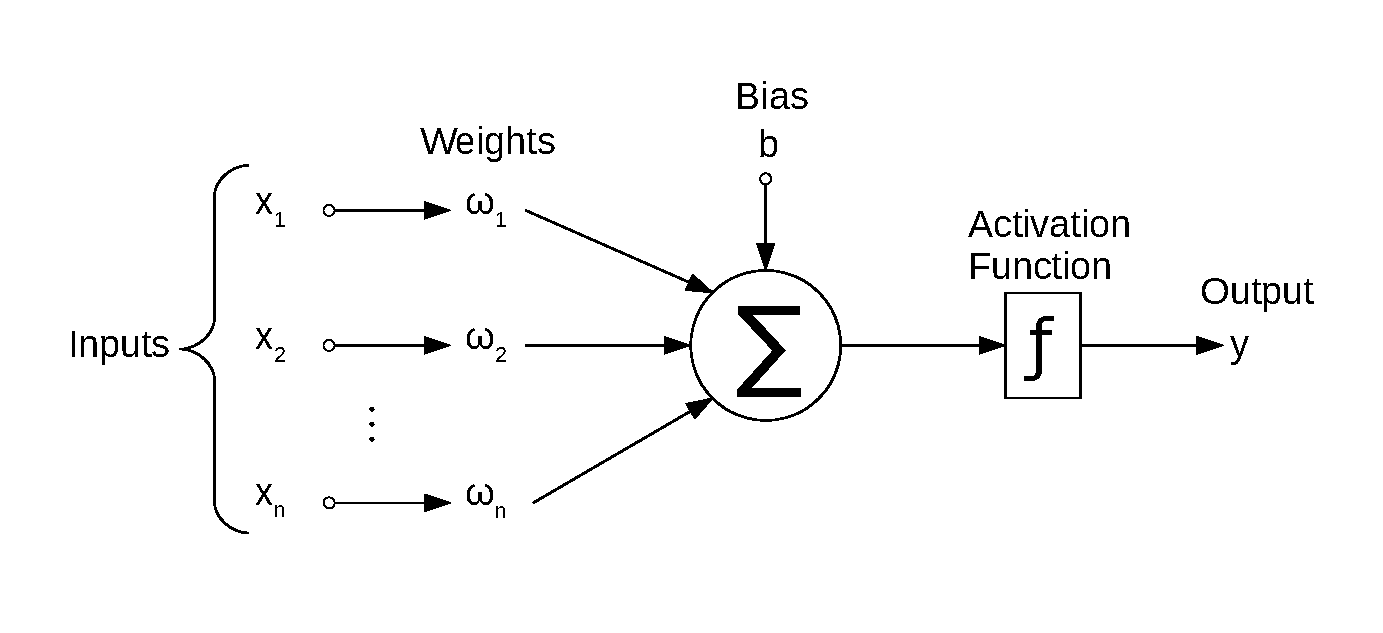
\includegraphics[scale=0.6]{neuron}
	\caption{Artificial neuron definition. Inputs are multiplied by the weights, all that is added together with a bias and passed to an activation function.}
	\label{fig:neuron}
\end{figure}

Multiple neurons stacked define a layer. The outputs from one layer connect to the inputs of another layer to form a neural network. There can be many layers in a single network, the term deep learning comes from the concept of having deep networks, which basically is a network with multiple inner layers. Figure \ref{fig:network} shows a simple network where every output from each layer connects to every input of the next layer. That is called a fully-connected or dense layer \cite{intro_cnn}.

\begin{figure}[thbp]
	\centering
	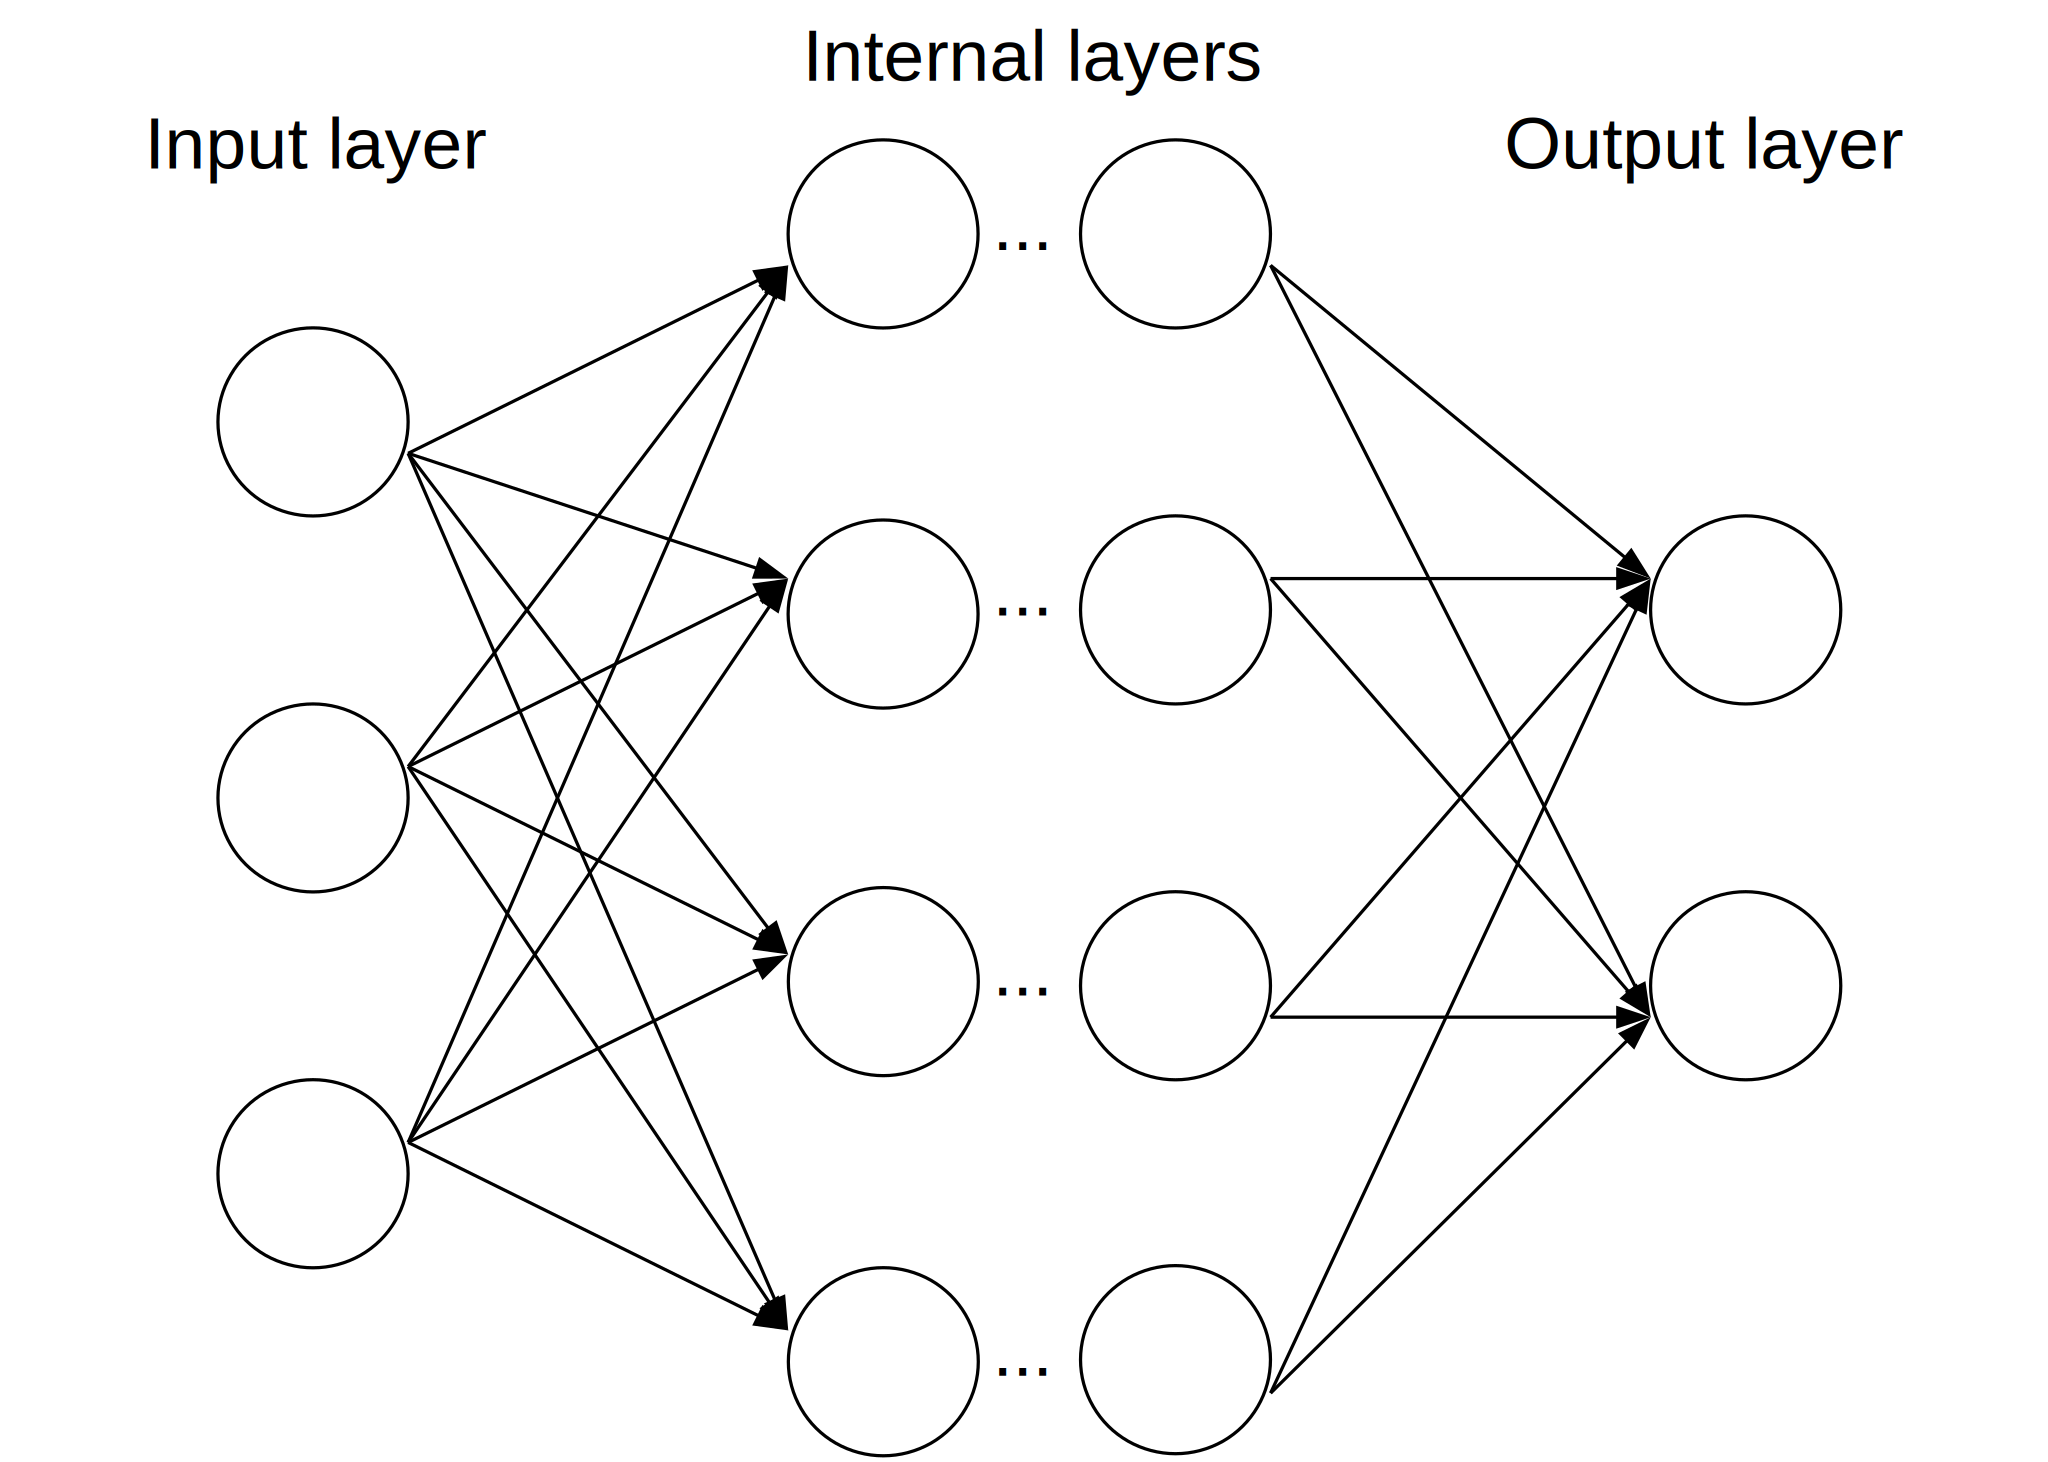
\includegraphics[scale=0.6]{network}
	\caption{Neural network made of fully-connected layers.}
	\label{fig:network}
\end{figure}

To train neural networks the weights and biases of the neurons are tweaked iteratively until the results that the network produces are good enough. On each training iteration the network is given a set of inputs and it will produce a set of outputs. Those outputs are compared against the desired or real values and an error function will produce a numerical value that will tell the network how good or bad was its prediction. That value is then propagated backwards and in each layer the weights and biases of the neurons will be adjusted to minimize the error. This process is called back-propagation.

\subsection{Convolutional Neural Networks}

Convolutional neural networks are a class of deep neural networks that are useful in computer vision fields. They are efficient at analyzing images for applications like image recognition and classification.

CNNs utilize image filters or kernels to do a transformation in a small group of pixels and obtain a result. Kernels are usually a square of a fixed amount of pixels, typical kernels are 3x3 or 5x5. The kernel is slid through the image and every pixel is multiplied by the kernel weights to produce one pixel for the next layer. Figure \ref{fig:cnn1} shows a visualization of a 3x3 kernel, in this example the pixels in the first layer will be multiplied by the corresponding weights of the kernel and those results will be added together to produce a single value for the next layer \cite{guide_cnn}.

\begin{figure}[thbp]
	\centering
	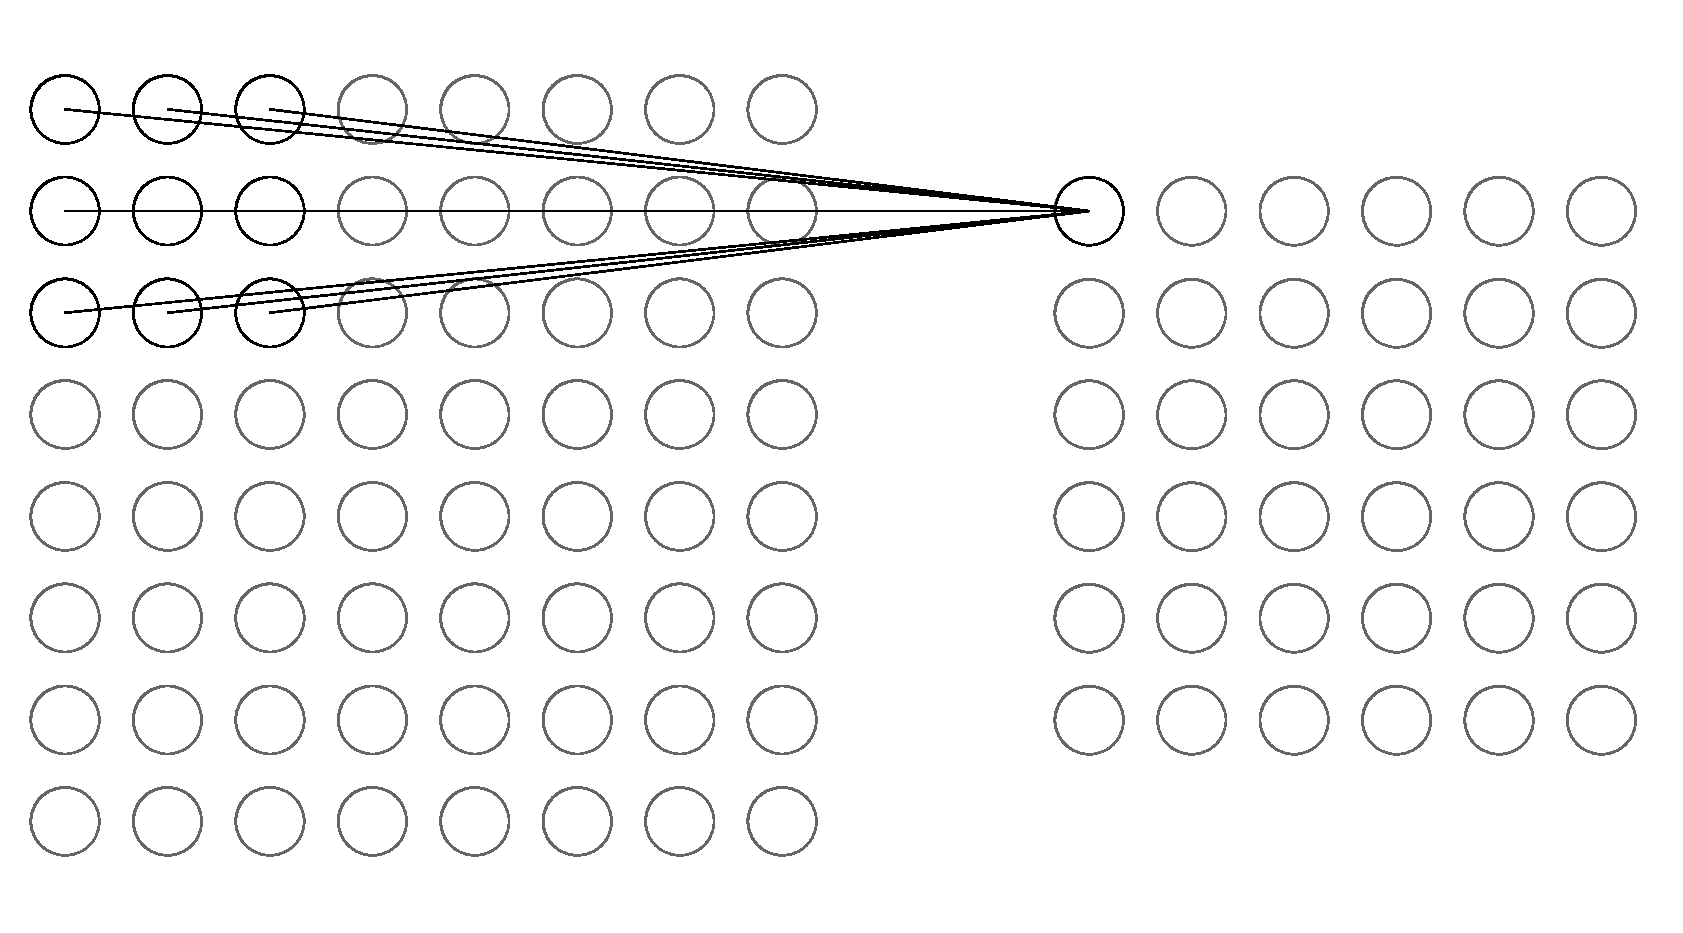
\includegraphics[scale=0.4]{cnn1}
	\caption{Visualization of a 3x3 kernel in a CNN.}
	\label{fig:cnn1}
\end{figure}

CNNs usually utilize multiple kernels at the same time to produce several images in each layer, this gives CNNs depth, which means that CNNs are not actually 2D matrices, but 3D cubes composed of 2D matrices. Usually, each level of depth highlights a special feature of the image, so they are called feature maps but they are also commonly called channels. Figure \ref{fig:cnn2} shows how a convolution layer looks like. In this example, the first layer contains three channels and the next one has five. All the feature maps in the second layer extract information from the first layer \cite{guide_cnn}.

\begin{figure}[thbp]
	\centering
	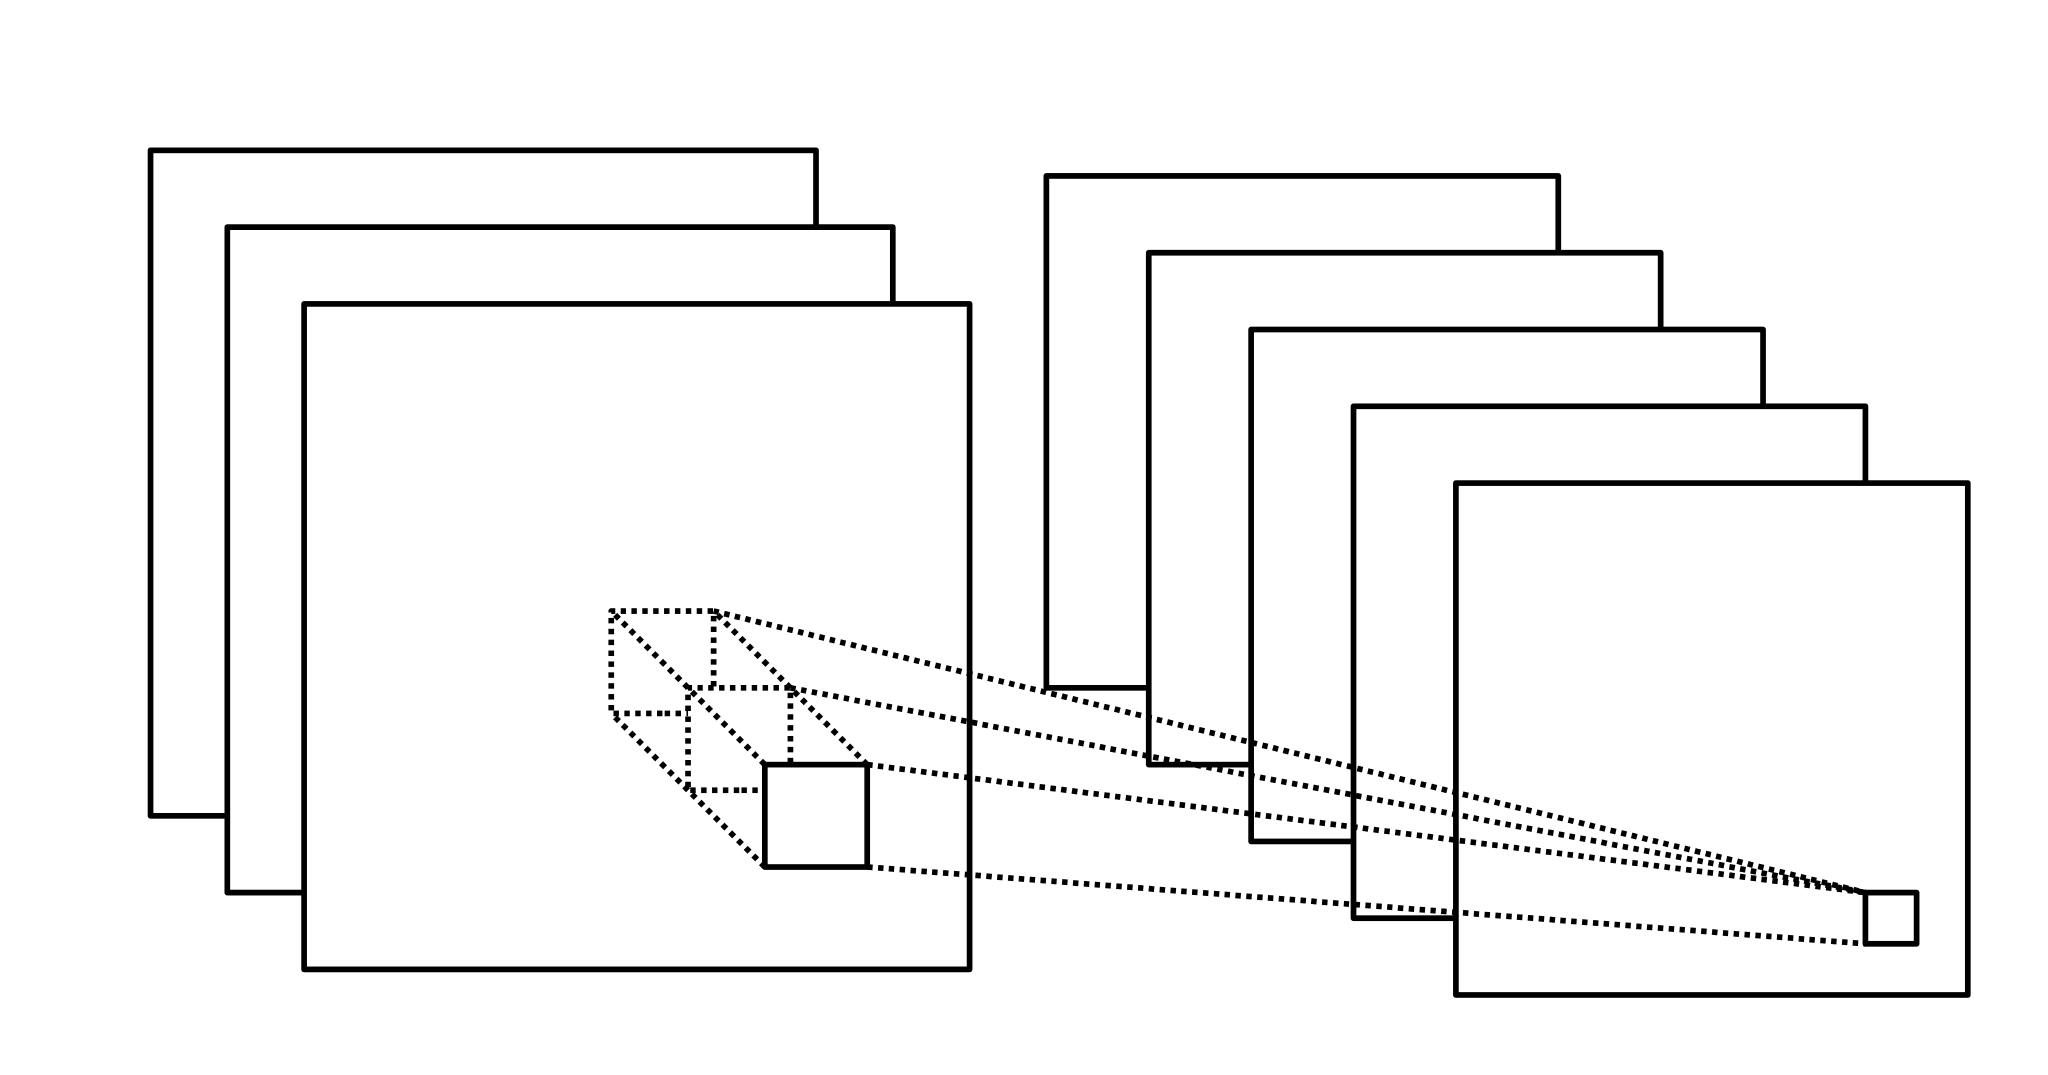
\includegraphics[scale=1.25]{cnn2}
	\caption{Visualization of a convolution layer.}
	\label{fig:cnn2}
\end{figure}

Because of how CNNs work, the trivial example of having a 1x1xC1 (height=1, width=1, channels=C1) layer followed by a 1x1xC2 layer and using a 1x1 kernel is the same as having a simple layer of \textit{C1} number of inputs followed by a fully-connected layer of \textit{C2} number of neurons. If the 1x1 kernel is kept but the layer dimensions are changed to an arbitrary height (H) and width (W) it would be the same as having HxW individual fully-connected layers. This can be exploited to run several full-connected neural networks in parallel in neural accelerators that are optimized for CNNs.

\subsection{Software-Level Optimizations and Approximations for Neural Networks}

\subsubsection{Pruning}

Pruning is the process of taking a neural network and removing some amount of neurons and/or connections (synapses). Usually this process is done intelligently by analyzing which neurons have weights close to zero and which connections affect the least the accuracy of the network. Once these neurons are identified the weights and biases are set to zero or removed completely from the network. Pruning can be done as a post-training optimization or it can be done during training \cite{prune1}.

Figure \ref{fig:prune} shows an example of how a neural network might look like before and after it is pruned. Pruning a neural network can have several positive effects. The network itself can be compressed and the file size is reduced. If the connections and neurons are removed completely the network itself is reduced in size and less operations need to be calculated when running the network. If the neurons are not removed and just zeroed the network might still run the operations, but if the hardware and/or software environment supports it, these zero weights can be identified and the operations can be skipped.

\begin{figure}[thbp]
	\centering
	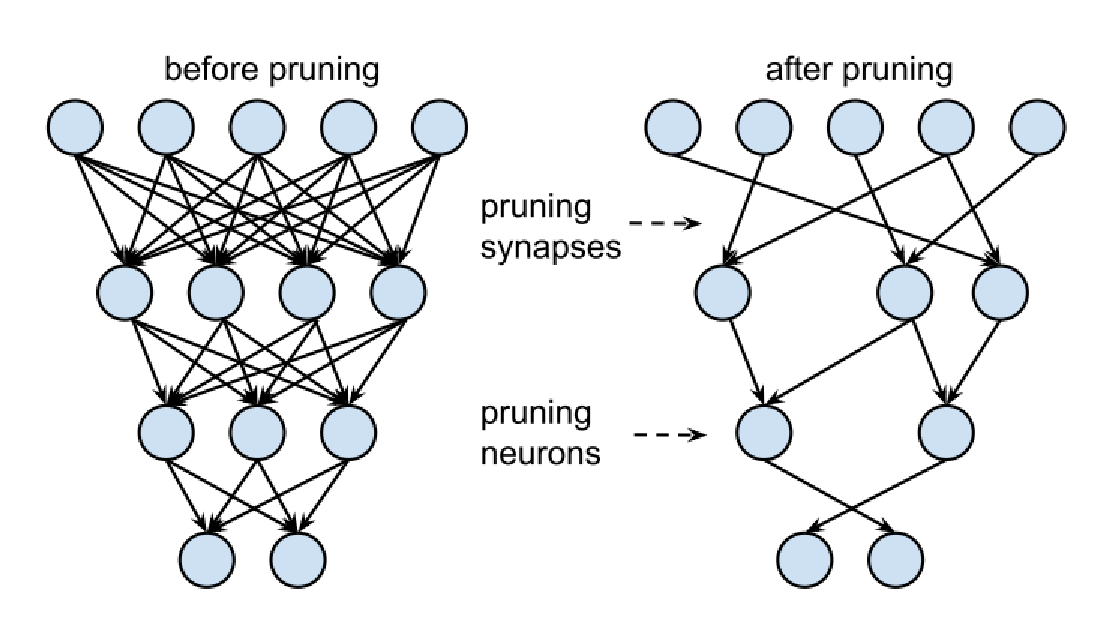
\includegraphics[scale=0.5]{prune}
	\caption{Example of neural network before and after pruning \cite{Han2015}.}
	\label{fig:prune}
\end{figure}

\subsubsection{Separable Convolution}

Sliding a kernel through a CNN requires many operations, and it increases dramatically when the depth of the CNN is large. Let's take the example of a CNN where the input image is 12 by 12 pixels, the kernel is 5 by 5, it has three channels, a stride is one and there is no padding (this sets the next layer size to 8 by 8 pixels). Let's also assume that the next convolutional layer has a depth of 256. If a normal convolutional layer is used, this means that a 5x5x3 kernel is slid through the image 256 times, which means that a total of 5x5x3x8x8x256=1,228,800 operations need to be done, see Figure \ref{fig:normal_conv}.

\begin{figure}[thbp]
	\centering
	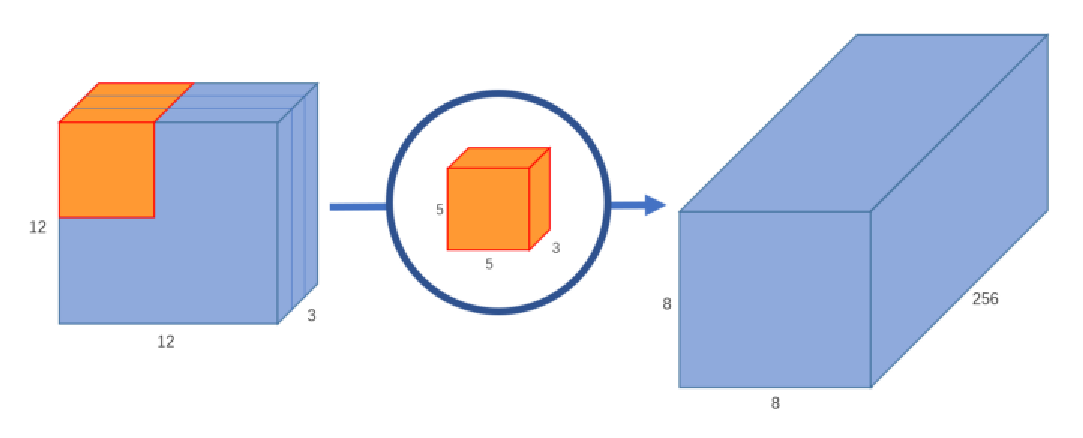
\includegraphics[scale=0.5]{normal_conv}
	\caption{Normal convolution example \cite{sep_conv}.}
	\label{fig:normal_conv}
\end{figure}

A normal convolution can be separated in two stages: a depthwise convolution and a pointwise convolution. Following the previous example, the depthwise convolution would have three kernels of shape 5x5x1 slid through the input image to create a 8x8x3 image, see Figure \ref{fig:depth_conv}. The output that we are seeking is 8x8x256, so now a pointwise convolution will be applied to make that shape. This means that 256 1x1x3 kernels will be applied to the 8x8x3 image created by the depthwise convolution and the result will be the desired 8x8x256 image, see Figure \ref{fig:point_conv}. The depthwise convolution needs 5x5x3x8x8=4,800 operations to be calculated and the pointwise convolution needs 1x1x3x8x8x256=49,152 operations. In total the separable convolution needs 53,952 operations, a much lower number than the normal convolution.

\begin{figure}[thbp]
	\centering
	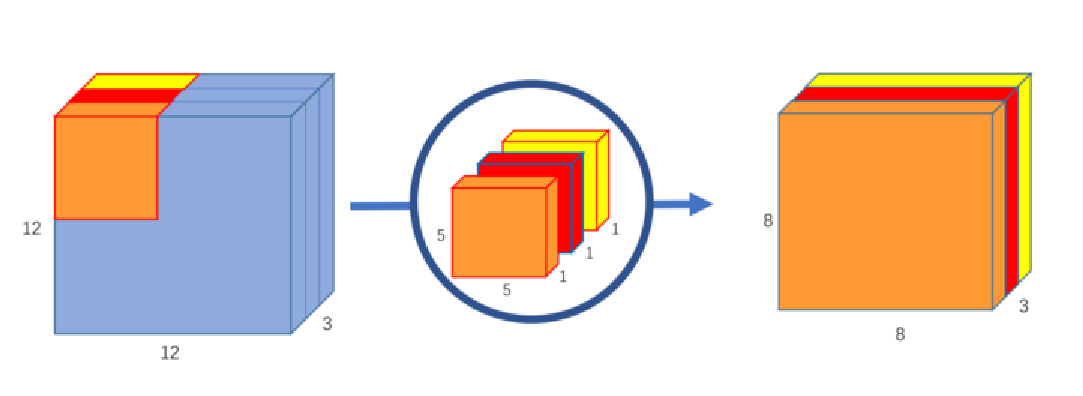
\includegraphics[scale=0.5]{depth_conv}
	\caption{Depthwise convolution example \cite{sep_conv}.}
	\label{fig:depth_conv}
\end{figure}

\begin{figure}[thbp]
	\centering
	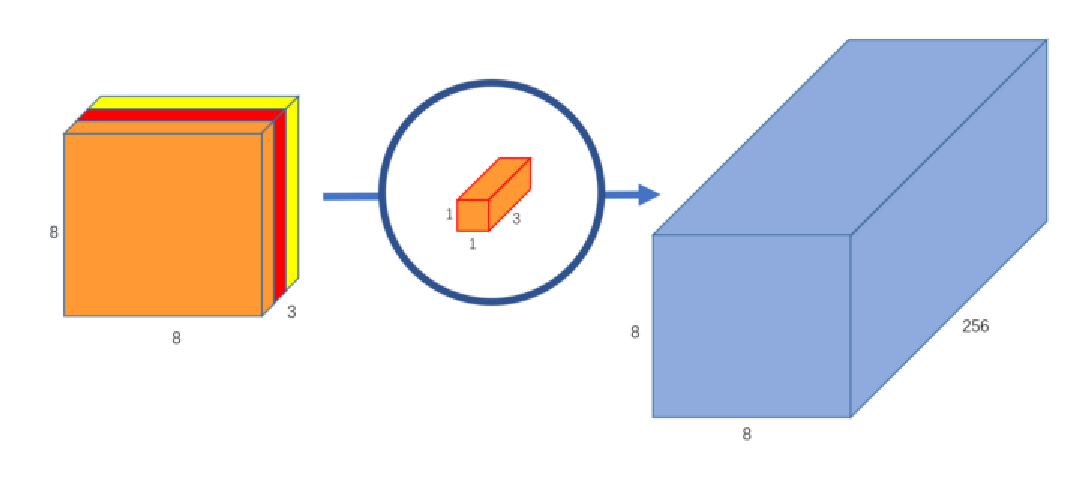
\includegraphics[scale=0.5]{point_conv}
	\caption{Pointwise convolution example \cite{sep_conv}.}
	\label{fig:point_conv}
\end{figure}

Conceptually, in a normal convolution the image is transformed 256 times, each time this is done 4,800 multiplications are needed. In the case of the separable convolution the transformation is done only once, during the depthwise convolution, so basically the transformed image is taken and it's just elongated to a depth of 256. This saves computational power since the image doesn't need to be transformed multiple times \cite{sep_conv}.

\subsubsection{Quantization}

In neural networks quantization is the concept of converting the weights in the neurons from a type with more precision to another type with less precision. Depending on the hardware, floating point operations can be slower and more power hungry than integer operation, so usually the process involves the conversion from floating point to integer. The quantization process is done to optimize the networks to run in hardware where integer operations can be executed faster and with less energy. Quantization doesn't only involve converting from floating point to integer, another optimization is to reduce the amount of bits for each weight, this can significantly accelerate the performance and energy efficiency of the network, specially if the hardware supports executing vector operations where several integer operations can be execute in parallel. The downside of quantization is that integer types can represent a lower range of numbers which means that when doing the computations precision is lost. If not done carefully quantizing a neural network can result in a significant loss of accuracy \cite{quant1}.

\section{Accuracy Estimation}

There are several methodologies on how to measure the error of results. In this section three different methods will be defined. These methods will be used in other chapters to measure the accuracy of the results obtained.

\subsection{Mean Absolute Percentager Error (MAPE)}

The first step to calculate this type of error consists in taking the absolute error for each measurement and dividing it by the corresponding expected (actual) value, this generates the relative error for each individual measurement. Then the sum of all the relative errors is taken and divided by the total number of measurements, generating the mean of all the relative errors \cite{DeMyttenaere2016}.

The formula that defines this error is the following:

\begin{equation}\label{eq:mape}
MAPE=\frac{1}{n}\sum_{t=1}^{n}\left| \frac{A_{t}-F_{t}}{A_{t}} \right|
\end{equation}

Where $A_t$ is the actual (real/expected) value and $F_t$ is the forecast (measured) value.

Although very popular and simple, this way of measuring error has some issues. Problems with this calculation start to be evident when the denominators are relatively small or zero. Checks need to be added when doing the calculations in order to avoid dividing by zero, in which case the error is set to 1 (100\%). Also, when the forecast values are too low, the percentage error can't exceed 100\%, but when they are too high there is no upper limit.

\subsection{Weighted Mean Absolute Percentage Error (WMAPE)}

This is an alternative to MAPE that alleviates the issue of small or zero denominators. It does it by separating the sums and calculating the absolute error of all the measurements first and then dividing by the sum of all the actual values. Another way of viewing this is substituting the $A_t$ denominator in formula \ref{eq:mape} with the average of all the actual values in the series \cite{wmape}.

\begin{equation}\label{eq:wmape}
WMAPE=\frac{1}{n}\frac{\sum_{t=1}^{n}\left| A_{t}-F_{t} \right|}{\sum_{t=1}^{n}A_{t}}=\frac{1}{n}\sum_{t=1}^{n}\left| \frac{A_{t}-F_{t}}{\bar{A}_{t}} \right|
\end{equation}

Were

\begin{equation}\label{eq:actual_vals_average}
\bar{A}_{t}=\frac{1}{n}\sum_{t=1}^{n}A_{t}
\end{equation}

The only disadvantage of this error measurement is that it can potentially hide or smooth out a small amount of big errors due to the averaging of the denominators.

\subsection{Mean Squared Error (MSE)}

This error calculates the mean of the squares of the absolute errors. It follows the following formula \cite{mse}:

\begin{equation}\label{eq:mse}
MSE=\frac{1}{n}\sum_{t=1}^{n}\left( A_{t}-F_{t} \right)^{2}
\end{equation}

This error measurement is good at showing big errors and at the same time hiding small errors, all this due to the squaring. The disadvantage is that the final measurement is absolute, not relative. This means that it is not suitable for comparing against other applications where the data range could be different.

\section{The OpenVINO Toolkit}

OpenVINO is a toolkit that facilitates programmers to utilize Intel hardware to do inference of neural network models. There are two main components to the toolkit: the Model Optimizer and the Inference Engine.

The Model Optimizer is a tool that facilitates the transition between the training and deployment environment. It performs model analysis and transforms the models for optimal execution in Intel hardware. It is composed of a series of scripts that take as input a saved model in one of the supported formats. The Model Optimizer can transform models from the following frameworks: Caffe, Tensorflow, MXNet, Kaldi and ONNX. The output of the Model Optimizer is called the Intermediate Representation (IR) of the network. The IR is composed of a pair of files that describe the mode: an XML file that describes the topology of the network and a binary file that contains the weights and biases of the neurons. Once the IR file is generated, it can be loaded onto a piece of hardware using the Inference Engine \cite{openvino_toolkit}.

\begin{figure}[thbp]
	\centering
	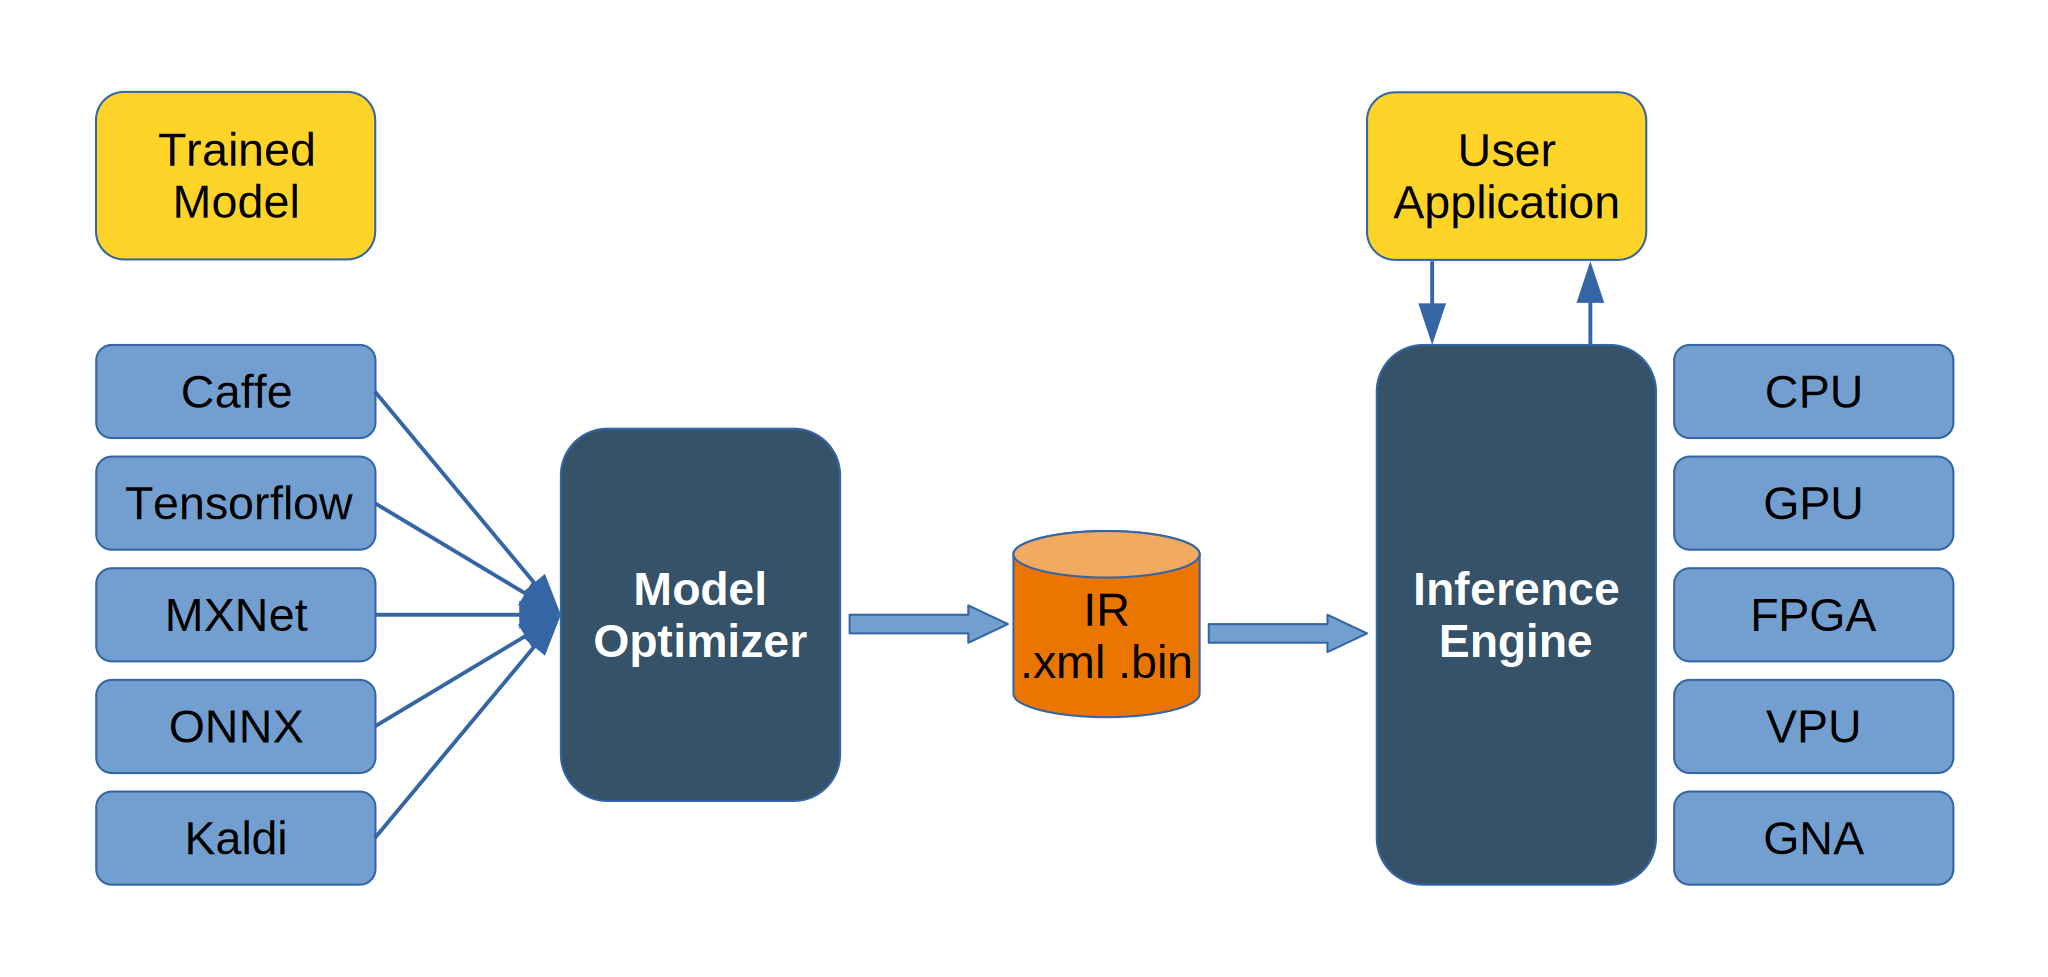
\includegraphics[scale=0.55]{openvino}
	\caption{OpenVINO workflow \cite{openvino_toolkit}.}
	\label{fig:openvino}
\end{figure}

Summary of the common workflow for using the Inference Engine API:

\begin{enumerate}
    \itemsep0em
	\item Create Inference Engine Core object
	\item Read the Intermediate Representation 
	\item Prepare inputs and outputs format
	\item Compile and Load Network to device
	\item Set input data
	\item Execute
	\item Get the output
\end{enumerate}
\item

The Inference Engine is a set of C++ libraries that provide an API to do inference on the different supported platforms (CPU, GPU, VPU, FPGA or GNA), it even supports heterogeneous inferencing using different pieces of hardware at the same time. The process of using the libraries to do inferencing requires the following steps. First, the user needs to create a \textit{core} object and load the IR files of the model. Then the network needs to be compiled and loaded into the target device. After that an \textit{infer request} object needs to be created, this will have a method called \textit{Infer} that will tell the hardware to act on the input data. Finally, the inputs and outputs need to be defined, an input and an output buffer are created. For each inference the input buffer needs to be filled with the input data and once the inference is done, the results can be accessed through the output buffer and the output data can be copied somewhere else for future use or can be analyzed in place and discarded \cite{openvino_toolkit}.

  \chapter{Literature Review}
\label{ch:review}

\section{Use of Neural Networks to Accelerate Error-\\Tolerant Applications}

In \cite{Esmaeilzadeh2012}, and algorithmic transformation, called the Parrot transformation, is proposed. It is a way of selecting regions of imperative code and training a neural network to mimic it, then a specialized hardware accelerator, a neural processing unit, is utilized to run the transformed code.

Figure \ref{fig:NPU_flow} shows the full workflow to utilize the algorithmic transformation technique. The programmer needs to annotate the code to indicate the compiler which parts to optimize and transform to a neural network. Then the compiler trains a neural network utilizing input data given by the user as well as some parameters to define the hyperparameters and architecture of the neural network. After that, code is generated that can run in an architecture that can configure the NPU to run the approximate parts of the program. Speedups ranging from 0.8x to 11.1x were achieved, as well as energy reductions ranging from 1.1 to 21.1. The experiments were run using the MARSSx86 simulator.

\begin{figure}[thbp]
	\centering
	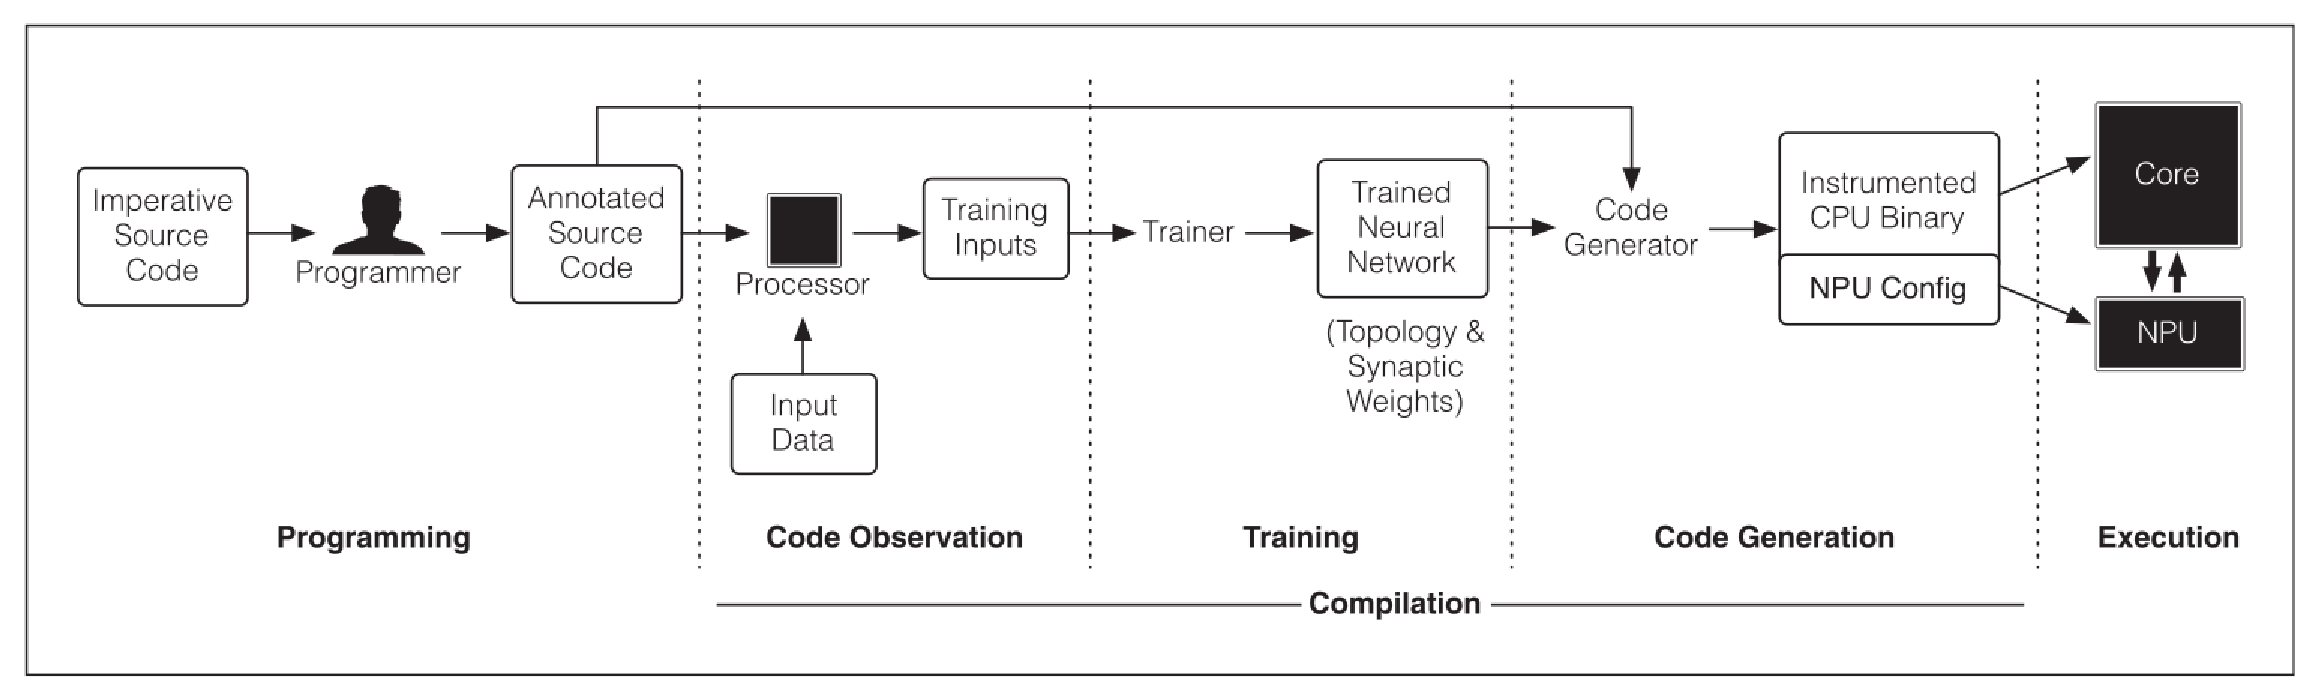
\includegraphics[scale=0.3]{NPU_flow}
	\caption[Work flow for approximate computing using NPUs.]{Work flow for approximate computing using NPUs \cite{Esmaeilzadeh2012}.}
	\label{fig:NPU_flow}
\end{figure}

In \cite{Moreau2015a} and \cite{Moreau2015} a novel method to do approximate transformations to code is proposed. Specifically, in \cite{Moreau2015a}, a high-level overview of both the software and hardware solutions is presented. ACCEPT is a compiler framework for approximate programs. It extends the C and C++ syntax to incorporate an APPROX keyword that can be used to annotate data types. Based on the annotations it applies program transformations only for the approximate data. It identifies regions of code that are safe to approximate. Then it executes the program with test cases and records input-output data to train a neural network that mimics the code using the back-propagation algorithm. Finally, it generates a binary that replaces the original code with invocations to the NPU.

In \cite{Moreau2015}, the SNAPP NPU is presented, it is designed to work with the ACCEPT compiler framework. It evaluates multi-layer perceptron (MPL) neural networks, using an array of Processing Units (PUs). Each PU consists of a chain of Processing Elements (PEs), a sigmoid unit and local memories. A PE consists of a multiply-and-add module implemented on a DSP slice. The sigmoid unit applies the neural network’s activation function to outputs from the PE chain. Speedups from 1.46x to 38.12x were achieved. Energy savings were on the 0.54x to 20.04x range. The platform used was the ZYNQ ZC702, which includes a 2-core ARM Cortex-A9 and a Xilinx Artix-7 FPGA (TSMC 28nm).

\section{Optimization of Neural Networks Using Approximate Computing Techniques}

This section explores the work that has been done to optimize inference on neural networks using approximate computing and other techniques. This can be done either in software, hardware or both.

In \cite{Venkataramani2015} a new technique is proposed that transforms a neural network into an approximate version of it that can run in a specialized hardware designed for it. They demonstrate that by utilizing this technique energy efficiency can be improved up to 1.92 times with little loss ($<$ 0.5\%).

Spiking neural networks are a new generation of neural networks that more closely mimic natural neural networks. In \cite{Sen2017}, the authors propose AxSNN, a new effort to apply approximate computing to improve the energy efficiency of SNNs. AxSNN achieved energy improvements of up to 3.62X using a specialized approximate accelerator.

In \cite{Peng2018} a novel method of training approximate neural networks is proposed. This method deploys two neural networks, an approximator and a predictor. These work together to guarantee the quality of the results. These optimized networks improve training time, have better energy efficiency and have less error than the non-approximate equivalent.

Pruning and quantization are techniques that can be helpful to improve performance and energy efficiency in neural networks. In \cite{Hanif2018} several case studies are presented which leverage these software level techniques as well as the use of approximate multipliers implemented in hardware to perform weighted sum operations.

In \cite{Sarwar2018} two algorithm level approximations are explored: lowering the network complexity and pruning. The first one consists of simply reducing the number of layers and/or neurons per layer with the objective to achieve improvements in energy efficiency without hurting the accuracy too much. Similarly, pruning removes certain connections in the neural network and reduces the complexity. In the same paper the authors also propose hardware level approximations: an approximate multiplier for neural computation and a voltage-scaled approximate memory for on-chip synaptic storage.

\section{Neural Network Accelerators}

The use of algorithmic transformations clearly show improvements to speed and power consumption, this is great but it can't be efficiently done in the real world unless those computations can be offloaded to an accelerator that can execute neural networks fast and with low power. This section will describe the Cambricon and Myriad accelerators, which are available commercially.

In \cite{Liu2016}, Cambricon, an instruction set architecture for neural networks is presented. The Cambricon ISA focuses on three areas: data-level parallelism, customized vector/matrix instructions and using on-chip scratchpad memory (instead of vector registers) to provide flexible width for each data access. It provides four types of instructions: computational (arithmetic and others for matrix/vector/scalars), variable-size data transfer (load/store/move for matrix/vector/scalars), logical (compare/logic for vector/scalar) and control (jump, conditional branch).

Using the Cambricon ISA, the Cambricon-X NPU is described at \cite{Zhang2016}. Cambricon-X's architecture consists on a control processor (CP), a buffer controller (BC), two neural buffers (NBin and NBout) to store input and output neurons, a direct memory access module (DMA) and a computation unit (CU) which contains multiple processing elements (PEs). The BC selects needed neurons for each PE from local neuron buffers based on the loaded instructions which are decoded by the CP, and transfers those neurons to PEs for efficient local computation.

The Movidius Myriad I is the first generation visual processing unit (VPU) designed by Movidius. It is designed for power-efficient computation. It has eight highly specialized cores focused in SIMD (single instruction multiple data) processing called SHAVEs (streaming hybrid architecture vector engines). The SHAVE processors are vector VLIW (very long instruction word) processors designed to crunch complex vision and imaging algorithms at high performance and low power. Each SHAVE core has assigned 128 Kbyte slices of SRAM memory, for a total of 1 MB. This memory is arranged in a CMX (connection matrix) topology. It also has 128 Kbytes of L2 cache which can be partitioned into independent caches. The chip runs at a top frequency of 200 MHz, with the memory clocked at 133 MHz \cite{Ionica2015}.

The Myriad 2 is the second generation of VPUs designed by Movidius. It now features twelve vector processors (SHAVEs) and double the memory (2 MB). The SHAVE processors are a new and improved version (3.0). The L2 cache is also doubled, getting it to a total of 256 Kbytes. The SoC now includes a new SIPP (streaming image processing pipeline) computational imaging hardware accelerators. The SHAVE cores themselves offer a 5x performance increase, now clocked at 600 MHz. On top of that the SIPP hardware accelerators can provide 15-25x additional performance \cite{Moloney2014}.

\begin{figure}[thbp]
	\centering
	\includegraphics[scale=0.35]{myriad_x}
	\caption[Myriad X VPU Architecture.]{Myriad X VPU Architecture \cite{myriad_vpus}}
	\label{fig:myriad_x}
\end{figure}

The Myriad X is the third generation of Movidius VPUs. The SHAVE processors count is increased to sixteen and the internal memory to 2.5 MB. It now also includes a dedicated deep neural network processing unit: the Neural Compute Engine, which can improve computations up to 10x \cite{myriadx}. The operating frequency received a bump to 700 MHz. Figure \ref{fig:myriad_x} shows a diagram of the Myriad X architecture. Table \ref{tab:myriad_vpus} compares the hardware specifications of the Myriad 2 and Myriad X VPUs. The most viable way of obtaining the Myriad VPUs is through the Intel Neural Compute Stick. The first generation used the Myriad 2 VPU and the latest iteration uses the newer Myriad X VPU. This is simple USB3 stick that plugs into any device and allows for offloading of neural network computations at a very low power. \cite{ncs2}

\begin{table}[thbp]
	\centering
	\caption[Movidius Myriad Family VPUs.]{Movidius Myriad Family VPUs \cite{myriad_vpus}}
	\label{tab:myriad_vpus}
	\resizebox{\textwidth}{!}{%
		\begin{tabular}{|c|c|c|}
			\hline
			& \textbf{Myriad 2}                                                                                             & \textbf{Myriad X}                                                                                                                   \\ \hline
			Compute Capacity             & \textgreater{}1 TOPS                                                                                 & \textgreater{}4 TOPS                                                                                                       \\ \hline
			Vector Processors            & 12x SHAVE Processors                                                                                 & 16x SHAVE Processors                                                                                                       \\ \hline
			CPUs                         & \begin{tabular}[c]{@{}c@{}}2x LEON4 cores\\ (RISC; SPARC V8)\end{tabular}                            & \begin{tabular}[c]{@{}c@{}}2x LEON4 cores\\ (RISC; SPARC V8)\end{tabular}                                                  \\ \hline
			On-chip Accelerators         & $\sim$20 image/vision processing accelerators                                                        & \begin{tabular}[c]{@{}c@{}}20+ image/vision processing accelerators\\ Neural Compute Engine (DNN accelerator)\end{tabular} \\ \hline
			Neural Network Capability    & \begin{tabular}[c]{@{}c@{}}1st Gen DNN Support\\ (Up to 100 GFLOPS)\end{tabular}                     & \begin{tabular}[c]{@{}c@{}}Neural Compute Engine\\ (Up to 1 TOPS)\end{tabular}                                             \\ \hline
			On-chip Memory and Bandwidth & \begin{tabular}[c]{@{}c@{}}2 MB\\ (400GB/sec)\end{tabular}                                           & \begin{tabular}[c]{@{}c@{}}2.5 MB\\ (450GB/sec)\end{tabular}                                                               \\ \hline
			DRAM Support                 & \begin{tabular}[c]{@{}c@{}}Max: 8Gb\\ LPDDR2 (533MHz, 32-bit)\\ LPDDR3 (933MHz, 32-bit)\end{tabular} & \begin{tabular}[c]{@{}c@{}}Max: 16Gb\\ LPDDR4 (1600MHz, 32-bit)\end{tabular}                                               \\ \hline
			DRAM Configurations          & \begin{tabular}[c]{@{}c@{}}1Gbit LPDDR2 (MA215X)	\\ 4Gbit LPDDR3 (MA245X)\end{tabular}               & \begin{tabular}[c]{@{}c@{}}No in-package memory (MA2085)		\\ 4Gbit LPDDR4 (MA2485)\end{tabular}                            \\ \hline
			Encoder/Codec                & VGA, 720p, 1080p, H.264 (software encoder)                                                           & \begin{tabular}[c]{@{}c@{}}M/JPEG 4K at 60Hz encoder\\ H.264/H.265 4K at 30Hz encoder\end{tabular}                         \\ \hline
			Key Interfaces               & \begin{tabular}[c]{@{}c@{}}12x MIPI lanes (DPHY 1.1)\\ USB 3\\ SPI\\ I2S\\ SD\\ 1GbE\end{tabular}    & \begin{tabular}[c]{@{}c@{}}16x MIPI lanes (PHY 1.2)\\ USB 3.1\\ Quad SPI\\ I2S\\ 2x SD\\ 10GbE\\ PCIe 3.0\end{tabular}     \\ \hline
			Process                      & 28nm HPC+/HPC/HPM (TSMC)                                                                             & 16nm FFC (TSMC)                                                                                                            \\ \hline
			Package                      & \begin{tabular}[c]{@{}c@{}}6.5mm x 6.5 mm (MA215X)\\ 8mm x 9.5 mm (MA245X)\end{tabular}              & 8.1mm x 8.8mm (MA2085, MA2485)                                                                                             \\ \hline
		\end{tabular}%
	}
\end{table}

\section{Review of Applications Using OpenVINO and Myriad VPUs}

To be able to program a neural processing unit such as the Myriad Family of devices, a programming framework needs to be provided to be able to access the hardware functions of the accelerator. Intel provides the OpenVINO toolkit to be able to program the Myriad accelerators. This section will review the work that has been done using the OpenVINO toolkit and the Movidius Myriad VPUs.

In \cite{Tiwari2019}, neural networks for image classification are deployed to the first generation of Intel Neural Compute Stick (NCS), which uses the Myriad 2 VPU. The results are compared against a Core i5-5200 CPU. The inference time in the CPU are lower (0.027 - 0.039 seconds) compared to what the NCS can provide (0.238 - 0.290). The advantage of the NCS is the power consumption, it uses 1.2 Watts while the CPU uses up to 69. This means that the performance per Watt is much better in the NCS (2.837 - 3.501 inferences/second/Watt) than in the CPU (0.371 - 0.536).

An analysis of the acceleration of neural networks inference on Intel processors is done in \cite{Andriyanov2020}. This study shows that using OpenVINO can significantly improve performance in Intel hardware. It compares a classical implementation with TensorFlow against an optimize version using OpenVINO. The results show that the OpenVINO version are significantly faster, with gains ranging from 88.07x up to 175.23x, with an average gain of 126.449x.

Low power devices with limited computing capacity can benefit substantially when offloading neural network computations to an external accelerator. This is what is demonstrated in \cite{Benelli2019}. A comparison is made between running inference in a Raspberry Pi 3 using the Caffe framework versus using the NCS running the model optimized with OpenVINO. The results show improvements in inference time and in energy per inference of up to 50\% with a loss of accuracy below 0.4\%.

In \cite{Castro-Zunti2020} a license plate segmentation and recognition system is tested. The baseline performance is 59 ms per inference, this is using TensorFlow on an Intel Xeon CPU with 12 cores. When the model is optimized using OpenVINO, the inference time is reduced to 14 ms. Transferring the application to a low-cost, low-power embedded system using the Raspberry Pi 3 and the Intel Neural Stick 2 means that the inference time is increased to 66 ms, which is only 7 ms more than the original un-optimized version running in the CPU.

One popular solution for accelerating neural networks is using FPGAs to offload the heavy processing. In \cite{Marantos2018}, the Xilinx Zynq-7000 was programmed, using HLS (High Level Synthesis), to run the SVM (Support Vector Machines) classifier. The same application was implemented using the Myriad 2 VPU and the results show that the power consumption is 80\% lower at the cost of doubling the execution time.

In \cite{Xu2018}, an application that uses 3D CNNs is deployed to three different platforms: an Nvidia Titan X GPU, an Intel i7-5930K CPU and the Movidius NCS. The performance in the GPU is highly superior, with an inference time of 0.5 ms, the NCS follows with 11 ms and lastly the CPU takes 13 ms. The efficiency of the NCS shines in this application, since the inference per seconds per watt is 75.75 vs 0.8 and 0.81 in the GPU and CPU respectively.

A lung nodule detection application was tested in several platforms in \cite{Mathew2019}. The results show a great reduction in inference time when running the application using OpenVINO versus Caffe. In an Intel i7 CPU the time improves from 7.5 seconds in Caffe to 0.2304 with OpenVINO. Even when deploying the application to the low-power NCS2, the inference time is reduced to 0.8142 seconds. The only tested configuration that is faster than OpenVINO is when running Caffe in an Nvidia GTX 1080 GPU.

  \chapter{Evaluation of OpenVINO and the Myriad X VPU with Error-Tolerant Applications when Applying Algorithmic Transformations}
\label{ch:ch1}

\section{Overview}

%This chapter explores the performance impact of how substituting a region of imperative code with a trained neural network that provides the same functionality in an approximate way. This area of approximate computing was previously explored in slightly different ways, utilizing code annotation to substitute the annotated piece of code with an inference call to a neural network. In \cite{Esmaeilzadeh2012}, an implementation is done by simulating an NPU that runs next to the CPU and at the same frequency. In \cite{Moreau2015a} and \cite{Moreau2015}, the inference is run in an FPGA which runs at one-fourth of the frequency of the CPU. In both cases the NPU is tightly coupled with the CPU.

The main objective of the work presented in this chapter is to explore the performance when doing approximate computing with neural networks utilizing OpenVINO, a free toolkit, as well as testing the capabilities of the Intel Neural Compute Stick 2 and the Movidius Myriad X VPU. This is a loosely coupled solution, it sacrifices latency and throughput for the flexibility of a plug-and-play device. The idea is to try to replicate what was done at an academic level and reproduce it in an environment with off-the-self components.

This chapter will focus on five applications from the AxBench suite of error-tolerant applications: blacksholes, inversek2j, jmeint, kmeans and sobel. The Black-Scholes model is a mathematical model for the dynamics of a financial market. Inversek2j is used in robotic and animation, it computes the angles of 2-joint robotic arms. Jmeint is a 3D gaming workload it determines if a pair of triangle coordinates intersect. Kmeans partitions a set of input points into a number of clusters. Sobel takes a color image and produces a gray-scale image highlighting the edges \cite{Yazdanbakhsh2016}.

\section {Tested Platforms Details}

Three different platforms were tested to obtain results on the selected applications: a desktop PC with an Intel CPU, a Raspberry Pi 3 Model B and a Raspberry Pi 4 Model B. Table \ref{tab:hw_sw_details} shows the details of each platform and Figure \ref{fig:phys_setup} shows pictures of the three platforms. For the neural network processing, the Intel Neural Compute Stick 2 was utilized.

These platforms were selected to have a range of different computing power. The low power Myriad X VPU will be compared against a powerful desktop CPU but also against much energy efficient systems like the ARM CPUs that the Raspberry Pi models include. For these experiments other compute devices could have been chosen, such as GPUs or FPGAs. The focus of this thesis is to evaluate a readily available low power off-the-shelf device like the NCS2 than can be paired with similar low power devices such as the Raspberry Pi, which are relevant nowadays with the growing importance of edge computing and Internet of Things (IoT).

\begin{table}[thbp]
\centering
\caption{Platform details.}
\label{tab:hw_sw_details}
\resizebox{\textwidth}{!}{%
\begin{tabular}{|l|l|l|l|l|l|l|}
\hline
\multicolumn{1}{|c|}{\textbf{Platform}}                          & \multicolumn{1}{c|}{\textbf{CPU}}                                                      & \multicolumn{1}{c|}{\textbf{GPU}}                                         & \multicolumn{1}{c|}{\textbf{RAM}}                             & \multicolumn{1}{c|}{\textbf{USB Ports}}               & \multicolumn{1}{c|}{\textbf{OS}}                                                              & \multicolumn{1}{c|}{\textbf{OpenVINO}} \\ \hline
Desktop PC                                                       & \begin{tabular}[c]{@{}l@{}}Intel Core i7-5930K\\ 6 C / 12 T\\ 3.5-3.7 GHz\end{tabular} & \begin{tabular}[c]{@{}l@{}}Nvidia\\ GTX 980\end{tabular}                  & \begin{tabular}[c]{@{}l@{}}16 GB DDR4\\ 2133 MHz\end{tabular} & \begin{tabular}[c]{@{}l@{}}USB 3\\ USB 2\end{tabular} & \begin{tabular}[c]{@{}l@{}}Ubuntu 20.04\\ \\ Kernel 5.4\end{tabular}                          & 2020.1                                 \\ \hline
\begin{tabular}[c]{@{}l@{}}Raspberry Pi 3\\ Model B\end{tabular} & \begin{tabular}[c]{@{}l@{}}Cortex-A53\\ 4 Cores\\ 1.2 GHz\end{tabular}                 & \begin{tabular}[c]{@{}l@{}}Broadcom\\ VideoCore IV\\ 250 MHz\end{tabular} & 1 GB                                                          & USB 2                                                 & \begin{tabular}[c]{@{}l@{}}Raspberry Pi OS\\ version 2020-05-27\\ \\ Kernel 4.19\end{tabular} & 2020.1                                 \\ \hline
\begin{tabular}[c]{@{}l@{}}Raspberry Pi 4\\ Model B\end{tabular} & \begin{tabular}[c]{@{}l@{}}Cortex-A72\\ 4 Cores\\ 1.5 GHz\end{tabular}                 & \begin{tabular}[c]{@{}l@{}}Broadcom\\ VideoCore IV\\ 500 MHz\end{tabular} & 4 GB                                                          & \begin{tabular}[c]{@{}l@{}}USB 3\\ USB 2\end{tabular} & \begin{tabular}[c]{@{}l@{}}Raspberry Pi OS\\ version 2020-05-27\\ \\ Kernel 4.19\end{tabular} & 2020.1                                 \\ \hline
\end{tabular}%
}
\end{table}

\begin{figure}[thbp]
	\centering
	\includegraphics[scale=0.75]{phys_setup}
	\caption{Physical setup for the tested platforms: Desktop PC, Raspberry Pi 4, Raspberry Pi 3.}
	\label{fig:phys_setup}
\end{figure}

\section{Methodology, Workflow and Implementation Details}

The whole purpose of the experiments run for this chapter is to have two versions for each application: one that runs the original imperative code in the CPU and another version that substitutes part of the code with a call to a neural network and that utilizes OpenVINO to do the inference on a supported device. This was achieved using the workflow shown in Figure \ref{fig:workflow}.

\begin{figure}[thbp]
	\centering
	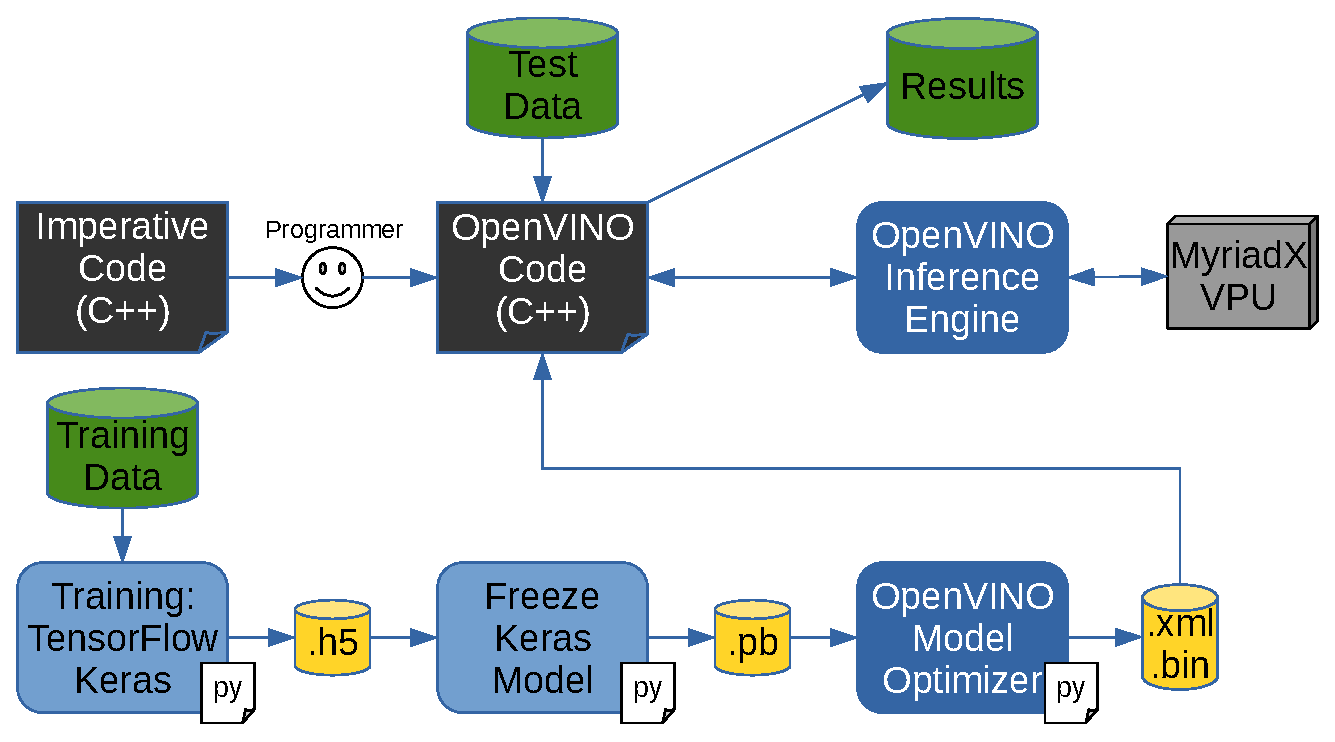
\includegraphics[scale=0.75]{workflow}
	\caption{Diagram of the workflow to apply the algorithmic transformation technique for approximate computing using the OpenVINO toolkit.}
	\label{fig:workflow}
\end{figure}

The starting point for this was the AxBench code for the applications that are going to be tested. AxBench is a general, diverse, and representative  set of benchmarks to evaluate different approximate computing techniques \cite{Yazdanbakhsh2016}. Since the benchmarks included in AxBench have been used in other relevant papers referenced by this work it was decided that it was the best set of applications to use as a baseline, that way it can be easily compared against previous works. These were selected because they represent a varied range of real-world error-tolerant applications from a wide range of domains. These applications are in line with evaluations done in previous work on approximate computing. Each application was written in procedural C++ originally. They will be re-written using an algorithmic transformation where a section of the code will be substituted to a call to run a neural network that will approximate the computations of the substituted code. For each of the applications the performance will be measured and compared against the original non-approximate application. The error for each of the applications will also be measured to see how much the results from the approximate version deviate from the non-approximate original version.

In the original AxBench applications whenever the user wants to substitute part of the code with an inference call, an annotation on the code is done and that will be substituted with a single call to the NPU. To be able to utilize OpenVINO's full potential the applications had to be modified to support batch processing. Instead of calling the inference on each iteration, the inputs to the neural network are stored in a buffer and when the buffer is filled a single call is made and all the stored inputs are all processed by a single inference call by OpenVINO. There are two main reasons to do it this way. One is that OpenVINO is a toolkit specialized for image processing and thus, optimized to handle CNNs. The same is true for the Myriad X VPU, the best performance is provided when the data is handled in batches in the form of a CNN. The second reason is that there is an overhead when sending the data to the device that is doing the inference. When utilizing the CPU for inference the overhead might not be as critical, but when utilizing a device like the NCS2, the input data needs to travel through an USB bus to the device and the output data needs to travel back to the PC and copied to the output buffer.

Creating and training the neural networks for the applications was done using Tensorflow version 1.15, the latest one compatible with OpenVINO version 2020.1. After training, the neural network is saved in a Keras \textit{.h5} format. To be able to load the network in OpenVINO this needs to be converted to OpenVINO's Intermediate Representation (IR). The \textit{.h5} format can't be converted directly, so a script is used to freeze the model and save it as a \textit{.pb} Tensorflow file, which can be used by OpenVINO's Model Optimizer to transform the model into the IR, which consists of a .bin and a .xml file, these contain the weights and biases and the topology of the network respectively. All applications were trained for a total of 1000 epochs.

As mentioned before, OpenVINO and the Myriad X VPU perform the best when processing the data in parallel in the form of a CNN. This means that for each application instead of handling one inference at a time as a fully connected network, multiple inferences are handled by emulating a multi-input fully connected networks as a CNN. For example, let us say that there is a fully connected neural network with an input of size 3, an output of size 2 and a hidden layer of size \textit{X}. This would be implemented in Tensorflow as a model with an input of three neurons, a hidden dense layer of \textit{X} number of neurons and an output dense layer with two neurons. To implement the same topology but in a CNN way where the network could process many inputs at a time, the first layer would be a 2D-convolutional layer with kernel of size (height=1, width=3), a stride of size (vertical=1, horizontal=3) and an output of \textit{X} channels, that connects to another 2D-convolutional layer now with kernel and stride both of size (1, 1) and an output size of 2 channels.

The code in Listing \ref{lst:code_dense} defines a fully-connected neural network with topology 3-X-2. All layers are using the Relu activation function.

\begin{minipage}{\linewidth}
\begin{lstlisting}[frame=single, tabsize=4, caption={Tensorflow example model using dense layers.},label={lst:code_dense},language=Python,captionpos=b]
	model = Sequential()
	model.add(Dense(X, activation='relu',
	                   input_shape=(3,)))
	model.add(Dense(2, activation='relu'))
\end{lstlisting}
\end{minipage}

The same topology can be created as a CNN, this time several neural networks are created, which allows for parallel inference. In the Listing \ref{lst:code_dense} example the input shape was a trivial one-element tuple with the number of inputs (3). In the CNN case, shown in Listing \ref{lst:code_cnn}, the matrix has a BxB size, so the input shape has height=B, width=Bx3 (the number of inputs for a single sample is 3) and channels=1. The hidden layer is a CNN layer with \textit{X} number of channels and has a simple (1,1) kernel and stride. The output is a 2-channel layer. The padding value `valid' means that no padding is added to the layer.

\begin{minipage}{\linewidth}
\begin{lstlisting}[frame=single, tabsize=4, caption={Tensorflow example model using convolutional layers.},label={lst:code_cnn},language=Python,captionpos=b]
	model = Sequential()
	model.add(Conv2D(X, (1,3), strides=(1,3),
	                           padding='valid',
	                           activation='relu',
	                           input_shape=(B,B*3,1)))
	model.add(Conv2D(2, (1,1), strides=(1,1),
	                           padding='valid',
	                           activation='relu'))
\end{lstlisting}
\end{minipage}

It is important to note that for this exploration each application was modified manually to be able to run with OpenVINO, this is because each one was implemented differently and it is not the objective of this exploration to automate the process of identifying the piece of code and creating the OpenVINO compatible inference calls nor training the neural networks automatically. Nonetheless, the following simplified code snippets show the basic ideas of how to implement the inference solution using the OpenVINO toolkit.

The code snippet in Listing \ref{lst:orig_code} shows the original procedural code. A simple loop iterates over all the inputs and for each one of them a error-tolerant function is called. The result is saved in an outputs array.

\begin{minipage}{\linewidth}
\begin{lstlisting}[frame=single, tabsize=4, caption={Procedural code of an error-tolerant function.},label={lst:orig_code},language=Python,captionpos=b]
	for (int i = 0; i < inputs.size(); i++) {
		outputs[i] = ErrorTolerantFunction(inputs[i]);
	}
\end{lstlisting}
\end{minipage}

The next code snippet shown in Listing \ref{lst:naive_code} uses a naive implementation of the code where a simple fully-connected neural network is used. The code execution is extremely slow when using OpenVINO and the NCS2 because for each input the data needs to travel through the USB3 bus, then the Myriad X does the inference and finally the data needs to travel back, which introduces latency on each call. For these simplified examples the assumption is that the neural network has one input and one output, hence the 0 index in the input and output buffers. This code is very similar to what the original AxBench applications implement.

\begin{minipage}{\linewidth}
\begin{lstlisting}[frame=single, tabsize=4, caption={Simple algorithmic transformation of an error tolerant-function using OpenVINO.},label={lst:naive_code},language=Python,captionpos=b]
	for (int i = 0; i < inputs.size(); i++) {
		input_buffer[0] = inputs[i];
		infer_request->Infer();
		outputs[i] = output_buffer[0];
	}
\end{lstlisting}
\end{minipage}

The code below in Listing \ref{lst:sync_code} shows a better implementation using CNNs. Here the data is processed in batches. Instead of iterating on every input the main loop iterates over blocks of inputs. On each block all the inputs for that corresponding block are copied to the input buffer. Then the inference is run and finally the results from the inference are copied back from the output buffer to the output array.

\begin{minipage}{\linewidth}
\begin{lstlisting}[frame=single, tabsize=4, caption={Algorithmic transformation of an error tolerant-function in batches using OpenVINO.},label={lst:sync_code},language=Python,captionpos=b]
	for (int i = 0; i < inputs.size(); i += BLOCK_SIZE) {
		for (int b = 0; b < BLOCK_SIZE; b++) {
			input_buffer[b] = inputs[i + b];
		}
		
		infer_request->Infer();
		
		for (int b = 0; b < BLOCK_SIZE; b++) {
			outputs[i + b] = output_buffer[b];
		}
	}
\end{lstlisting}
\end{minipage}

The final implementation, shown in Listing \ref{lst:async_code}, is the most efficient because it is asynchronous. Here the code doesn't have to wait for the inference to finish in order to move on to the next block. This implementation has a defined number of inference requests that can be happening in parallel. The flow is similar to the previous example, the difference is that the \textit{StartAsync} function doesn't wait for the inference results. At the beginning of each loop the code checks to see if the inference request (\textit{ir}) is ready and blocks until it is (doesn't block if it is not active). This is needed to free that particular inference request object. Once the inference is ready, the results are copied from the output buffer. Now the inference request object is inactive and can take a new request. The inputs are copied, the request is sent and the iteration number is saved in the \textit{iters} array. This last part is needed to be able to map the inference request to the block of inputs that was processed by that particular inference request when getting the results from the output buffer. After that, the inference request counter (\textit{ir}) is incremented to prepare for the next loop.

\begin{minipage}{\linewidth}
\begin{lstlisting}[frame=single, tabsize=4, caption={Most efficient implementation of algorithmic transformation of an error tolerant-function using OpenVINO.},label={lst:async_code},language=Python,captionpos=b]
	for (int i = 0; i < inputs.size(); i += BLOCK_SIZE) {
		if (infer_request_is_active_and_ready(
            infer_request[ir]
        )) {
			for (int b = 0; b < BLOCK_SIZE; b++) {
				outputs[iters[ir] + b] = output_buffer[ir][b];
			}
		}
		
		for (int b = 0; b < BLOCK_SIZE; b++) {
			input_buffer[ir][b] = inputs[i + b];
		}
		
		infer_request[ir]->StartAsync();
		iters[ir] = i;
		
		ir++;
		if (ir == max_ir)
			ir = 0;
	}
\end{lstlisting}
\end{minipage}

\section{Results}

\begin{table}[thbp]
	\caption{Neural network topologies.}
	%\begin{adjustbox}{width=\columnwidth,center}
	\centering
	\resizebox{\columnwidth}{!}{
		\begin{tabular}{|l|l|l|l|l|l|l|}
			\hline
			\textbf{}            & \multicolumn{2}{c|}{\textbf{NN 1}}      & \multicolumn{2}{c|}{\textbf{NN 2}}      & \multicolumn{2}{c|}{\textbf{NN 3}}      \\ \hline
			\textbf{Application} & \textbf{Topology} & \textbf{Parameters} & \textbf{Topology} & \textbf{Parameters} & \textbf{Topology} & \textbf{Parameters} \\ \hline
			blackscholes         & 6-20-1            & 161                 & 6-20-20-1         & 581                 & 6-20-20-20-1      & 1001                \\ \hline
			inversek2j           & 2-8-2             & 42                  & 2-8-8-2           & 114                 & 2-8-8-82          & 186                 \\ \hline
			jmeint               & 18-32-8-1         & 881                 & 18-32-16-8-1      & 1281                & 18-32-16-16-8-1   & 1553                \\ \hline
			kmeans               & 6-8-4-1           & 97                  & 6-8-6-4-1         & 143                 & 6-8-6-6-4-1       & 185                 \\ \hline
			sobel                & 9-8-1             & 89                  & 9-8-8-1           & 161                 & 9-8-8-8-1         & 233                 \\ \hline
		\end{tabular}
	}
	\label{tab:nn_topologies}
	%\end{adjustbox}
\end{table}

In this section, the results from several different measurements will be shown. Starting with figure \ref{fig:pc_rel_perf}, the results from running the original code in the CPU are compared with running the approximate version in the same CPU and using the Myriad accelerator in the NCS2. All applications except for kmeans showed an improvement in performance when running the approximate version in the CPU. Unlike that result, none of the applications showed an improvement in performance when running in the Myriad VPU. This result was expected, since the Myriad VPU is a very low power unit and simply cannot rival an i7 CPU running at a much higher frequency and with many cores.

\begin{figure}[thbp]
	\centering
	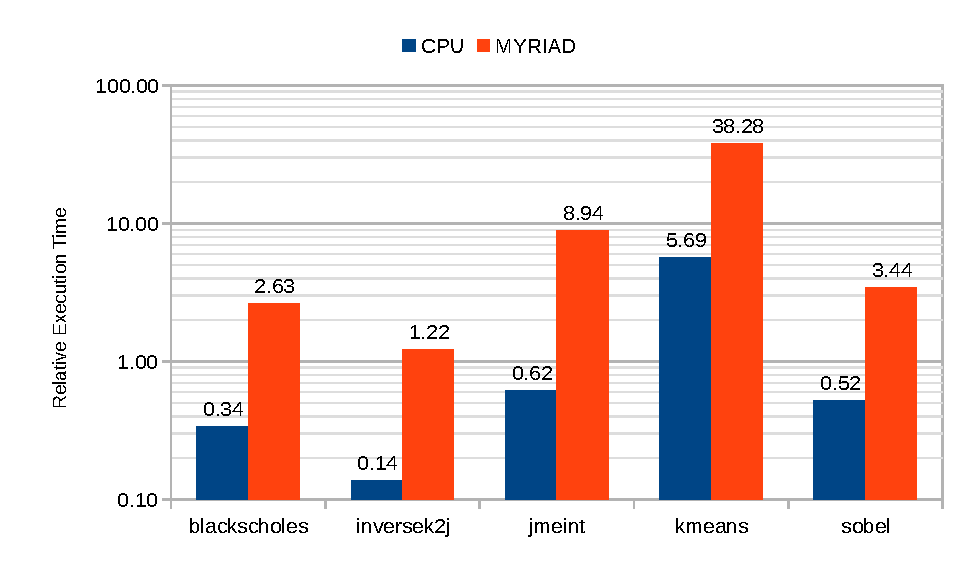
\includegraphics[scale=0.75]{pc_rel_perf}
	\caption{Execution time of the approximate version of the applications relative to the procedural version, tested in a desktop PC.}
	\label{fig:pc_rel_perf}
\end{figure}

Figure \ref{fig:pc_rel_perf_nn_sizes} shows the same results as Figure \ref{fig:pc_rel_perf}, but with three flavors of the same neural network. The first one (NN 1) is the same one as figure \ref{fig:pc_rel_perf}, and constitutes the baseline result. The next two (NN 2 and NN3) are more complex variations with extra layers and extra parameters. Table \ref{tab:nn_topologies} shows the different network sizes. The objective of showing these results is to measure how performance is impacted when using bigger and more complex neural networks. As seen in the graph, blacksholes, inversek2j and sobel were the ones that followed a more lineal trend of complexity vs performance loss, while jmetint and kmeans didn't show much impact in performance relative to the network size. The topologies used for these networks were based on the examples that AxBench includes \cite{Yazdanbakhsh2016}.

\begin{figure}[thbp]
	\centering
	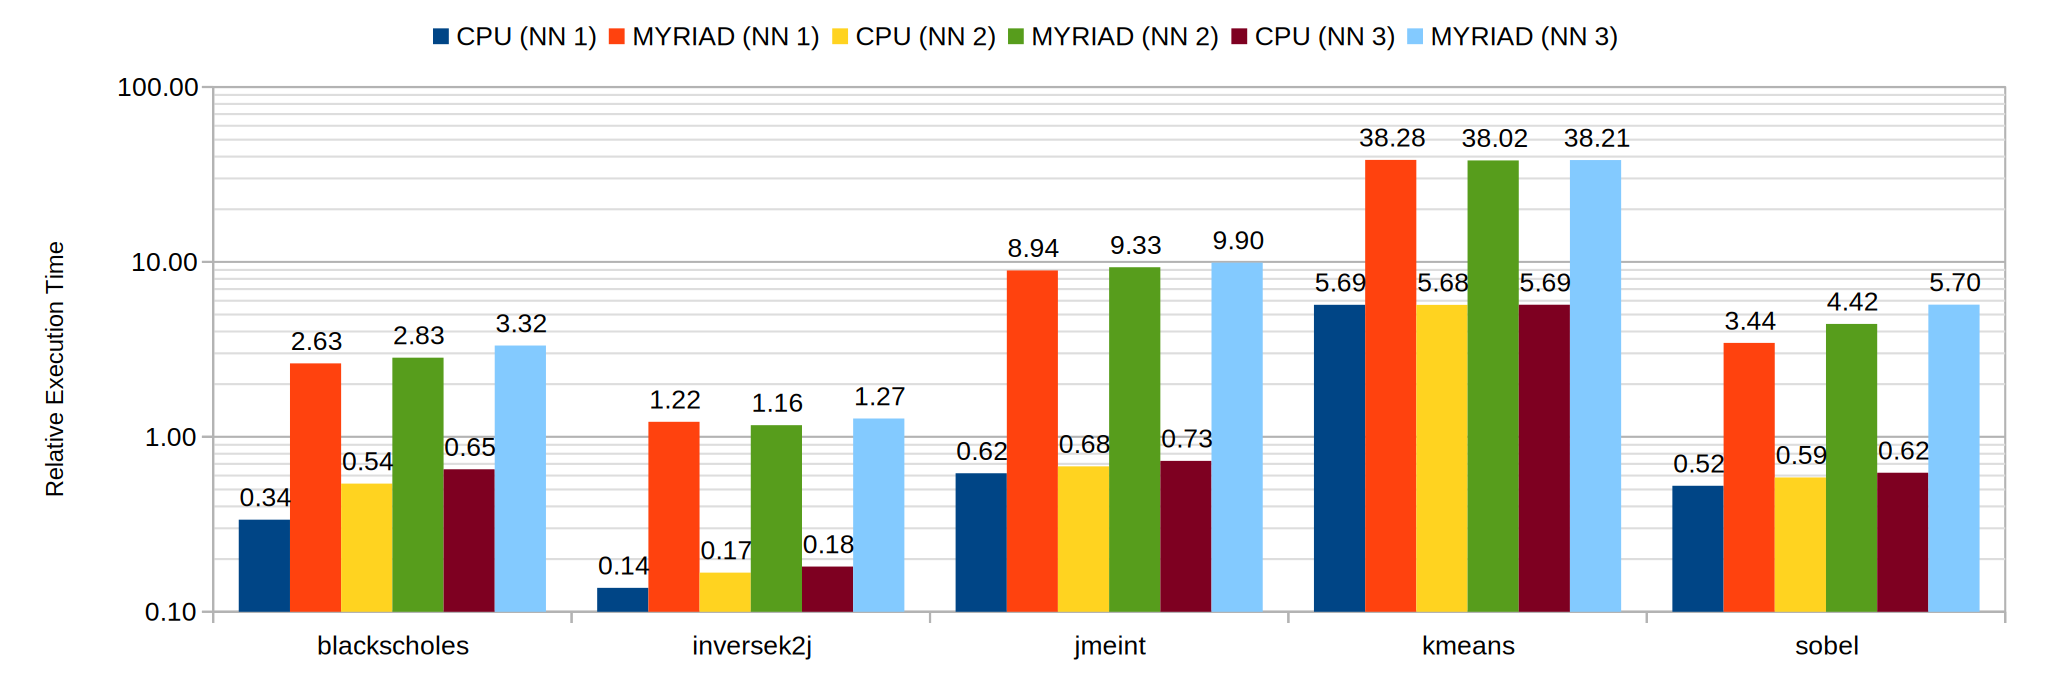
\includegraphics[scale=0.6]{pc_rel_perf_nn_sizes}
	\caption{Comparison of the relative execution time for different neural network sizes.}
	\label{fig:pc_rel_perf_nn_sizes}
\end{figure}

To see how different systems could benefit from utilizing the proposed approximate computing technique, it was tested on three different ones: a PC with an Intel CPU, a Raspberry Pi 3 and a Raspberry Pi 4. One noticeable result was that in the Raspberry Pi 3, the results were lower than expected. One of the reasons is that it only has USB2 ports and it cannot fully utilize the potential of the NCS2. To measure how much the USB2 hurts performance vs utilizing USB3, Figure \ref{fig:usb2} shows the relative slowdown when using USB2 vs USB3 in both the PC and the Raspberry Pi 4. On average, when running in USB3 the performance is 4.6 times better.

\begin{figure}[thbp]
	\centering
	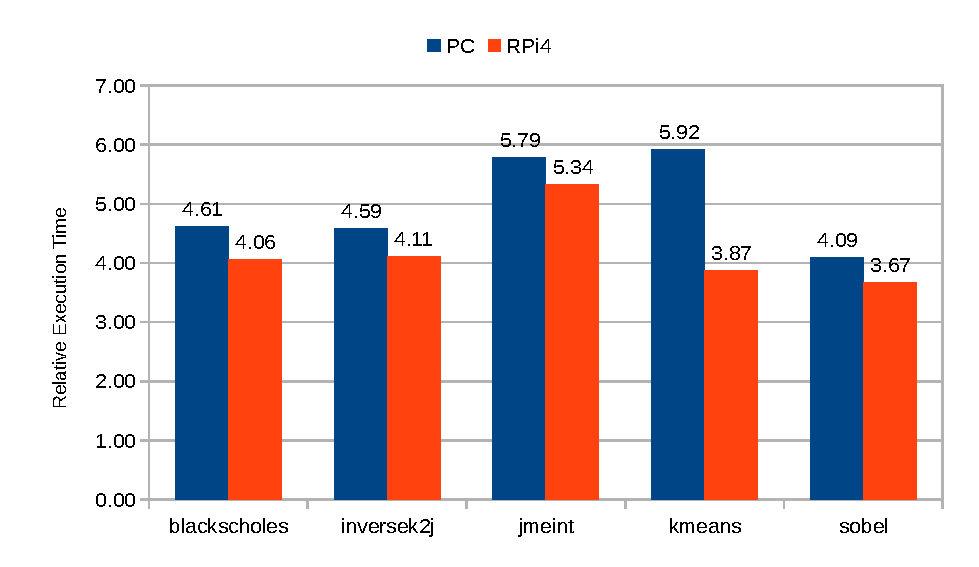
\includegraphics[scale=0.75]{usb2}
	\caption{Slowdown when connecting the NCS2 to a USB2 port.}
	\label{fig:usb2}
\end{figure}

On figure \ref{fig:rpi3_rel_perf} the Raspberry Pi 3 results are shown. Unfortunately, since this system only has a USB2 interface, the system is bottle-necked and most of the applications saw a slowdown compared to the non-approximate version. Only one application, inversek2j, showed an increase in performance using the approximate computing method. Since this system's CPU is slow the relative performance is not as bad as it could be. This shows that any embedded systems that want to benefit from an accelerator like the Myriad need to have a fast interface to reduce bottlenecks.

\begin{figure}[htbp]
	\centering
	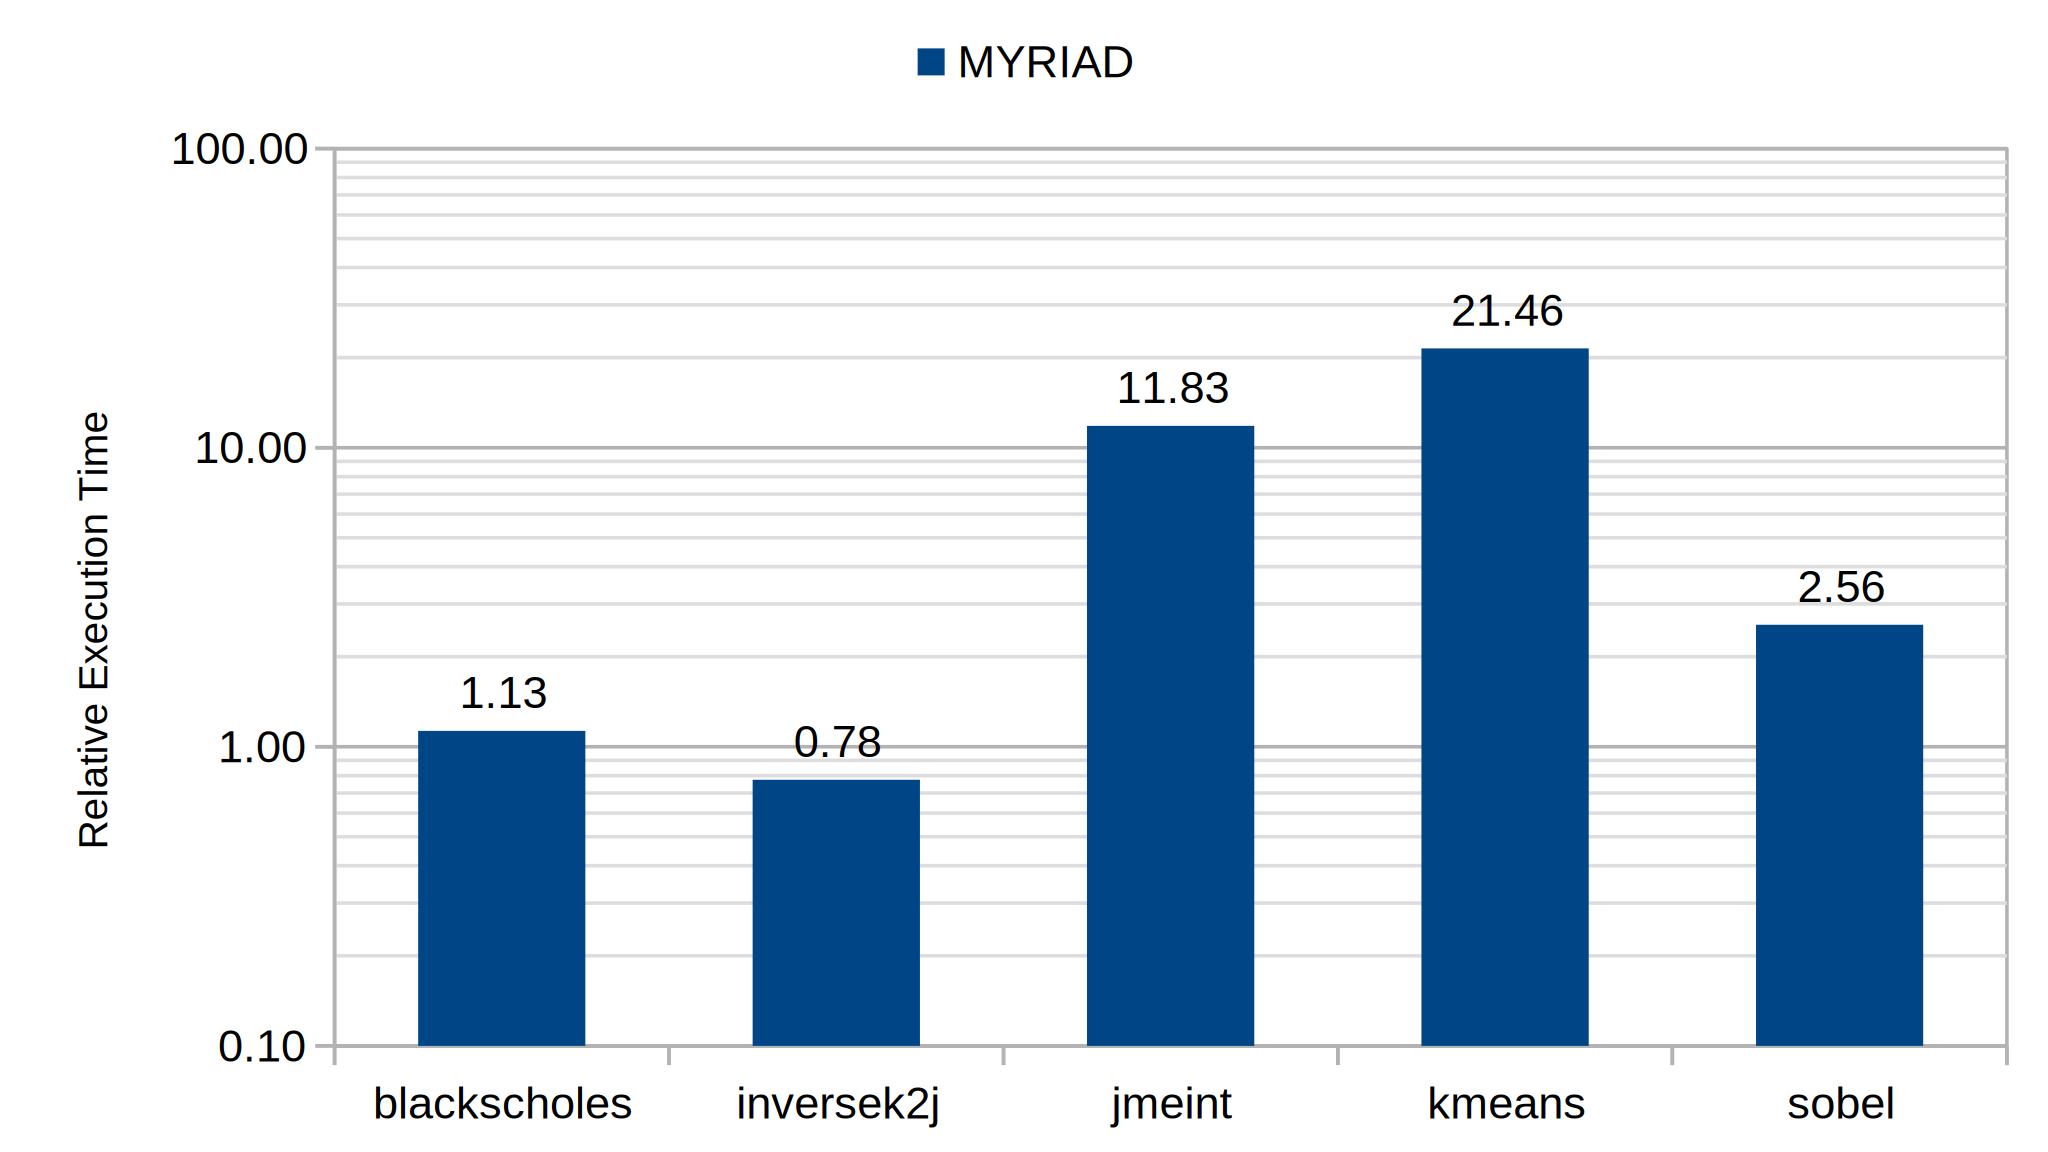
\includegraphics[scale=0.75]{rpi3_rel_perf}
	\caption{Execution time of the approximate version of the applications relative to the procedural version, tested in a Raspberry Pi 3 Model B.}
	\label{fig:rpi3_rel_perf}
\end{figure}

On Figure \ref{fig:rpi4_rel_perf} the results for the Raspberry Pi 4 are shown. Even though this system has a USB3 interface, only two applications showed an improvement in performance. This is because the system contains a CPU that can run the original code much faster. Except for kmeans, all the applications do show a relative improvement in performance compared to the Rapsberry Pi 3.

\begin{figure}[htbp]
	\centering
	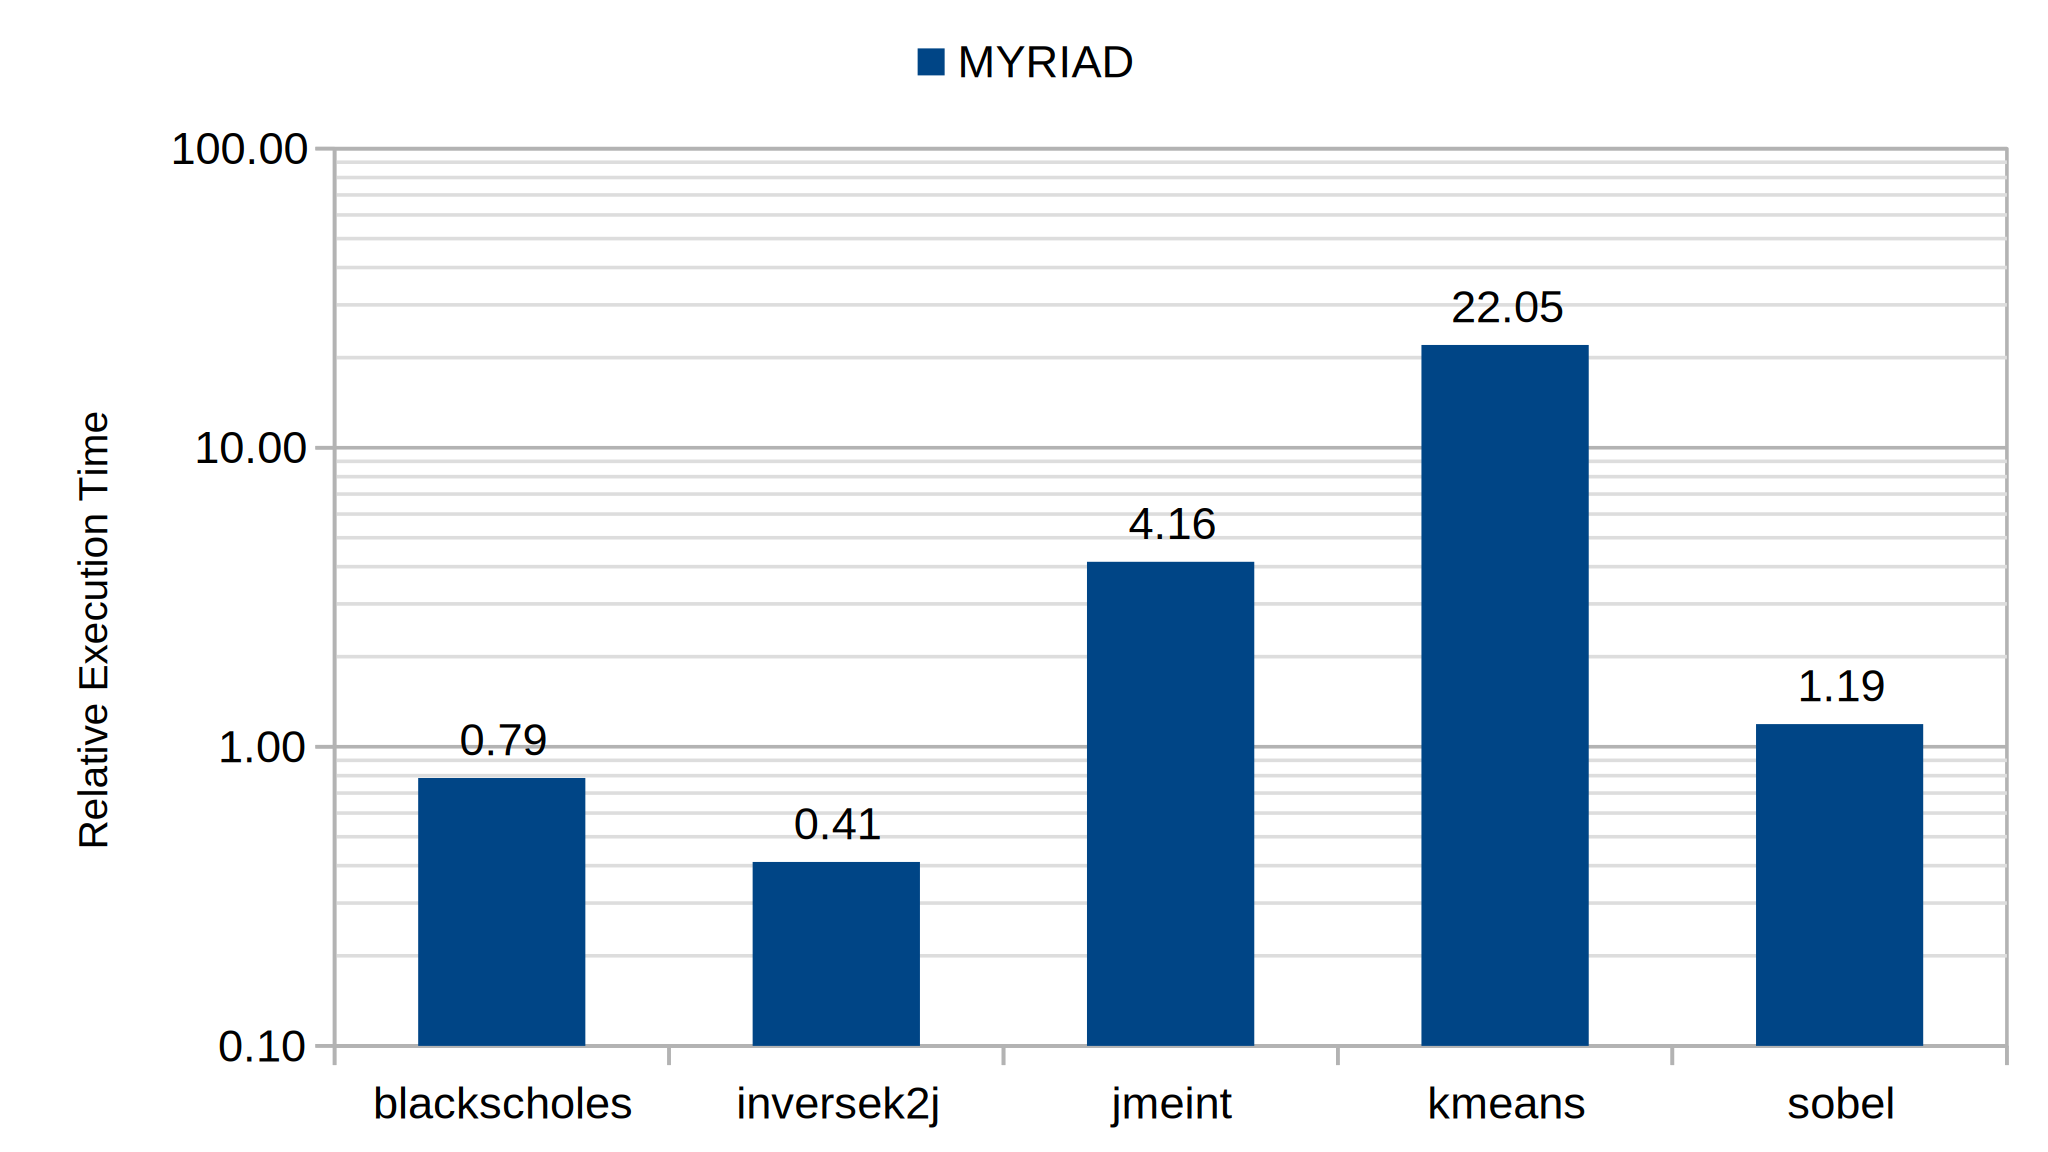
\includegraphics[scale=0.75]{rpi4_rel_perf}
	\caption{Execution time of the approximate version of the applications relative to the procedural version, tested in a Raspberry Pi 4 Model B.}
	\label{fig:rpi4_rel_perf}
\end{figure}

Next the results for the error measurements are shown, starting with the MAPE in Figure \ref{fig:mape}. The graphs for the error measurements all show the three different neural network sizes. Ideally, increasing the size and complexity of the network should reduce the error. The trend mostly follows that assumption, but there are some exceptions. In backscholes, when run in the Myriad VPU, increases in the most complex network. For sobel both the CPU and Myriad results show a degradation in the most complex network. From the graphs it can be concluded that for all the applications except kmeans after the second network there are diminishing returns. This means that there are redundant parameters in the network that are simply not needed or don't contribute significantly to it. The only application that really benefits from a more complex network is kmeans.

\begin{figure}[thbp]
	\centering
	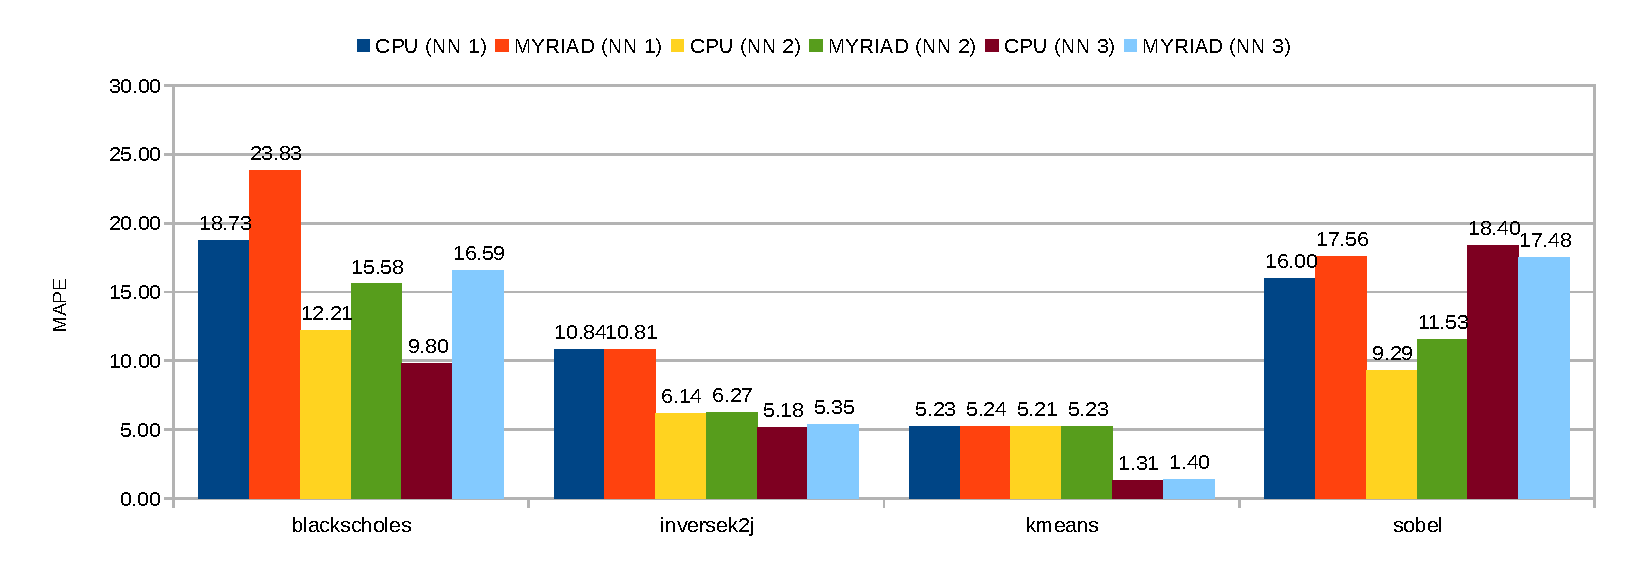
\includegraphics[scale=0.6]{mape}
	\caption{Mean absolute percentage error.}
	\label{fig:mape}
\end{figure}

Figure \ref{fig:wmape} shows the WMAPE and it follows the same trend as the MAPE results. The overall error when measuring the WMAPE is much lower, the reason is that the calculation doesn't punish results that are zero.

\begin{figure}[thbp]
	\centering
	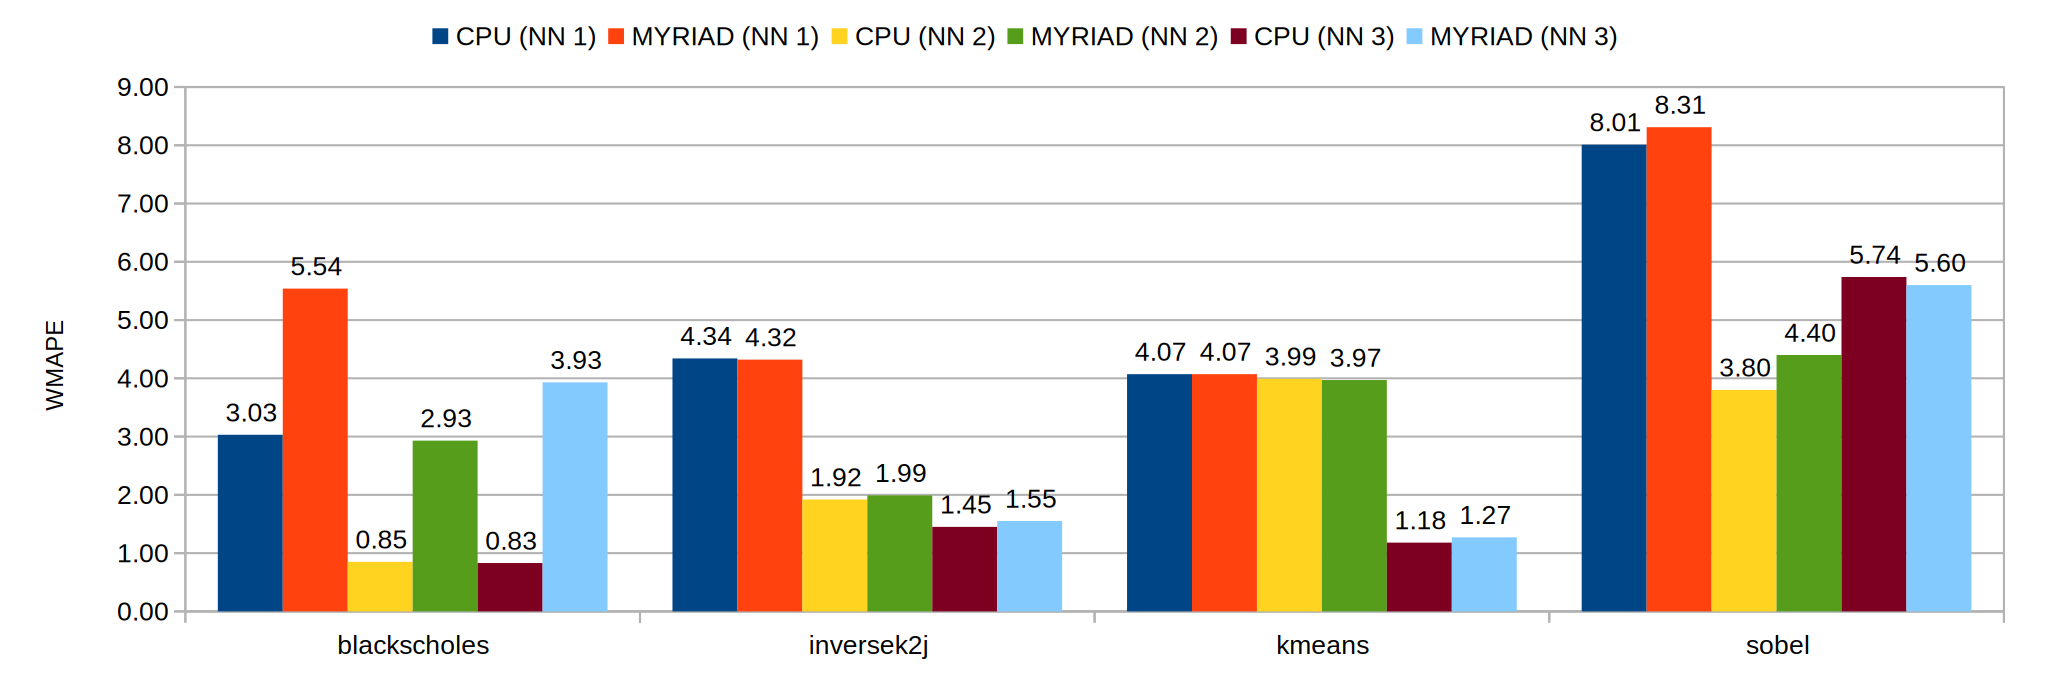
\includegraphics[scale=0.6]{wmape}
	\caption{Weighted mean absolute percentage error.}
	\label{fig:wmape}
\end{figure}

The normalized MSE is shown in figure \ref{fig:mse} and it also follows the same trend as the MAPE and WMAPE results.

\begin{figure}[thbp]
	\centering
	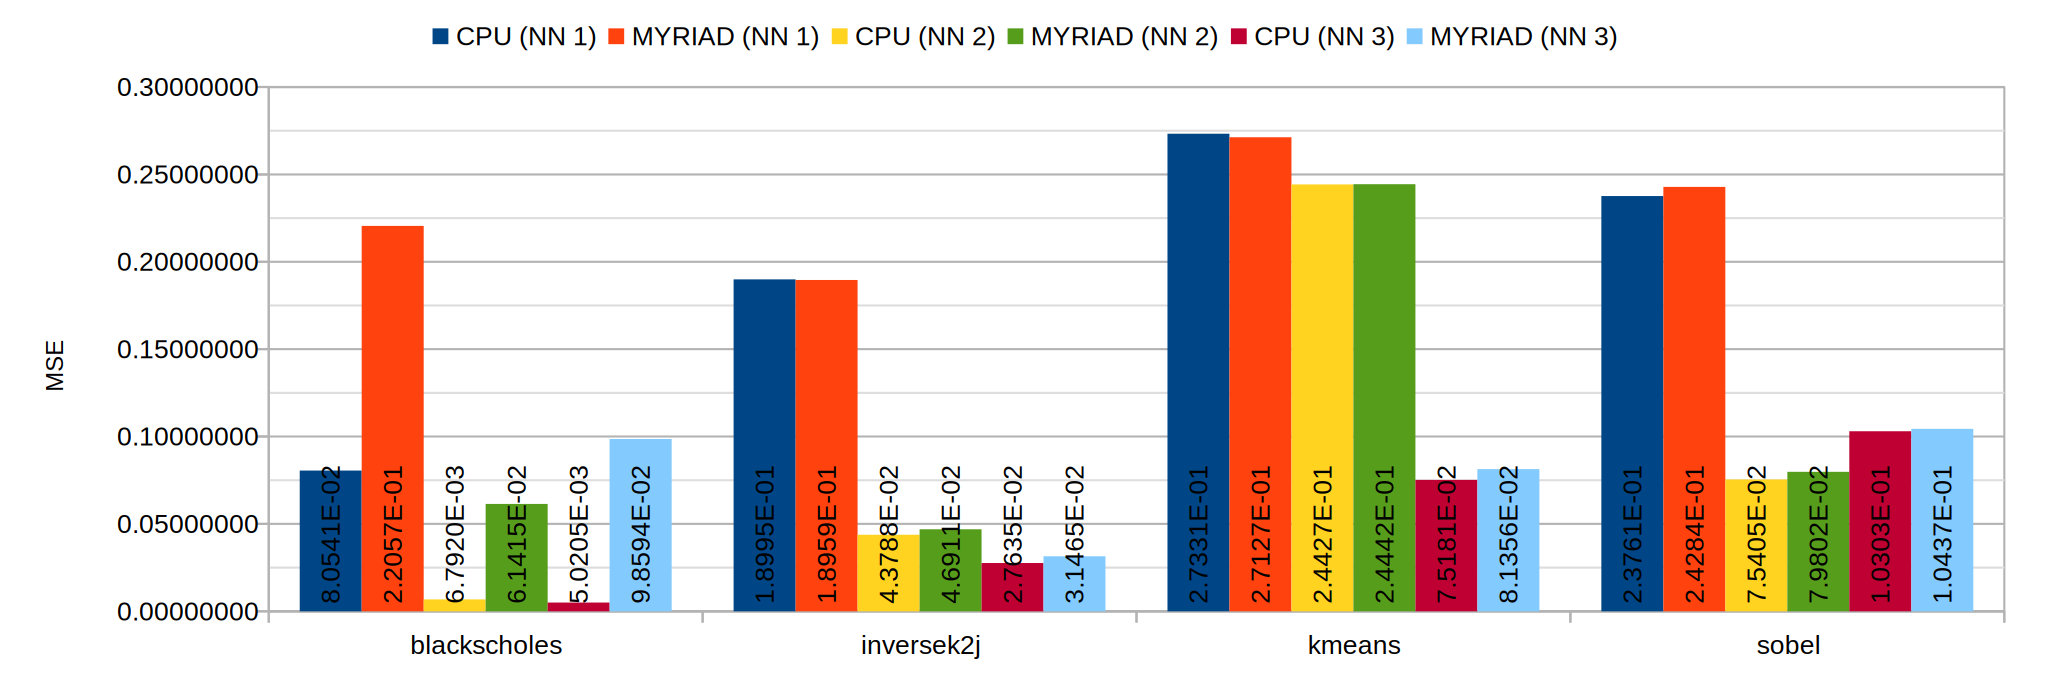
\includegraphics[scale=0.6]{mse}
	\caption{Mean squared error (normalized).}
	\label{fig:mse}
\end{figure}

Figure \ref{fig:perc_err} shows the error for the jmeint application which is measured differently. The results for jmeint are either 0 or 1. The error is the miss rate of the network, the opposite of the accuracy. There is a small benefit of using more complex network, but it shows diminishing returns when the complexity starts to grow.

\begin{figure}[thbp]
	\centering
	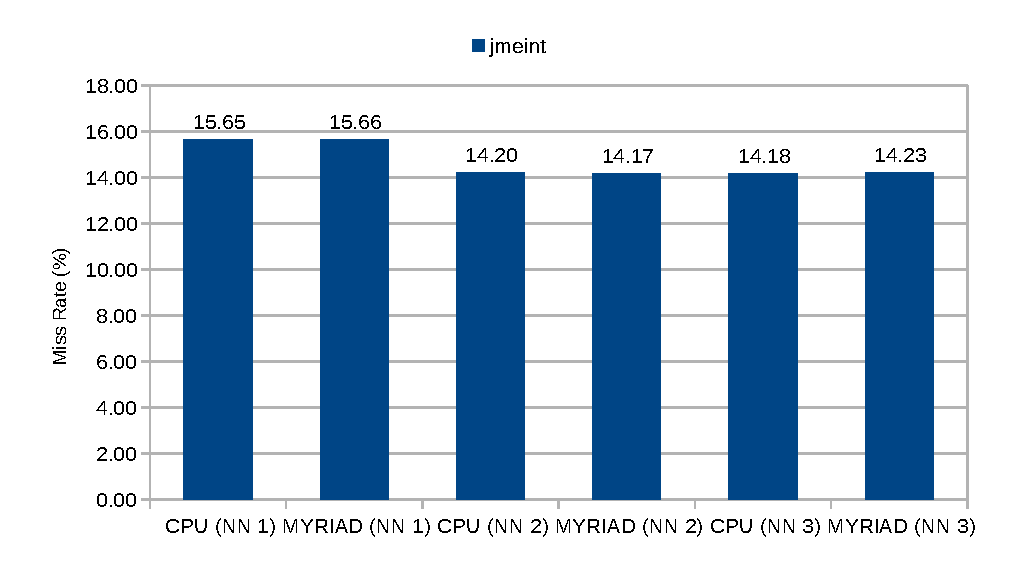
\includegraphics[scale=0.75]{perc_err}
	\caption{Error percentage (miss rate) for jmeint.}
	\label{fig:perc_err}
\end{figure}

In summary, the results were mixed. When using a powerful desktop PC, the results show that using the Myriad accelerator will not improve performance, although its low power could be beneficial in some applications. Using the Intel CPU itself to do the inference can improve the performance since the OpenVINO platform optimizes the model to utilize the CPU efficiently. The most interesting results involve low power platforms like the Raspberry Pi, in which case it is highly recommended that the device supports a high speed interface like USB3, since low speed interfaces significantly reduce the performance by creating a bottleneck when transferring the data. To consider the use of OpenVINO and the Myriad X VPU to accelerate error-tolerant applications thorough benchmarking has to be done to make sure that the specific application can benefit from the capabilities of the toolkit and the accelerator.
%The objective of this chapter was to improve the performance of error-tolerant applications by doing algorithmic transformations that could run in a neural accelerator. This objective was partially achieved since two out of five applications saw an improvement when running in the Raspberry Pi 4.

  \chapter{Optimizing Machine Learning Applications Using Approximate Computing Techniques}
\label{ch:ch2}

\section{Overview}

OpenVINO is designed with the objective to accelerate machine learning applications that use CNNs. The Myriad X VPU is tailored to accelerate vision applications, so it is also optimized to run CNNs. In this chapter, three applications are tested and a set of optimization techniques are explored to find how these applications can be run faster without hurting significantly the accuracy of the results. Three classification applications were selected for testing. The first one is audio classification, the data set consists of audio files with recordings of spoken digits. The second application is fruit classification with 131 different fruit categories. The third application consists of identifying different landscape scenes such as forests, buildings, mountains and others.

The next section describes the details of the selected machine learning applications that are tested. Table \ref{tab:app_summary} show the summary of the data-sets used in the applications. After that, the description of the details of the selected topologies for each application are presented. The methodology details are shared in the following sections: the selected approximate computing optimization techniques that are implemented and the different parameters that are measured when running the applications.

\section{Applications}

\begin{table}[thbp]
\centering
\caption{Applications Summary}
\label{tab:app_summary}
\begin{tabular}{|l|l|l|l|l|l|}
\hline
\multicolumn{1}{|c|}{\multirow{2}{*}{\textbf{Application}}} & \multicolumn{1}{c|}{\multirow{2}{*}{\textbf{Categories}}} & \multicolumn{3}{c|}{\textbf{Dataset Split}}                                                       & \multicolumn{1}{c|}{\multirow{2}{*}{\textbf{Size}}} \\ \cline{3-5}
\multicolumn{1}{|c|}{}                             & \multicolumn{1}{c|}{}                            & \multicolumn{1}{c|}{\textbf{Train}} & \multicolumn{1}{c|}{\textbf{Validation}} & \multicolumn{1}{c|}{\textbf{Test}} & \multicolumn{1}{c|}{}                      \\ \hline
Audio                                              & 10                                               & 2160                       & 240                             & 600                       & 64x64x1                                    \\ \hline
Fruit                                              & 131                                              & 50769                      & 16923                           & 22688                     & 100x100x3                                  \\ \hline
Scene                                              & 6                                                & 11929                      & 2105                            & 3000                      & 150x150x3                                  \\ \hline
\end{tabular}
\end{table}

\subsection{Audio Classification}

For this application the objective is to try to identify spoken digits. The dataset used is the Free Spoken Digit Dataset \cite{fsdd}. This dataset consists of 10 classes: all the digits from zero to nine. It is composed of 3000 recordings from 6 different speakers with different accents, this means that for each digit there are 50 recordings per speaker. The dataset itself is made from wav files. These wav files are converted to spectrograms before being used. This makes the classification process easier since now the dataset is in a 2D format which can be fed to a traditional 2D CNN and the problem can be treated in the same way as a image classification problem. The resulting spectrogram has the following properties: the \textit{x} axis represents time, the \textit{y} axis represents the frequency, and the pixel intensity, in gray-scale representation, represents the amplitude of a specific frequency at a given time (see Figure \ref{fig:specs}).

\begin{figure}[thbp]
	\centering
	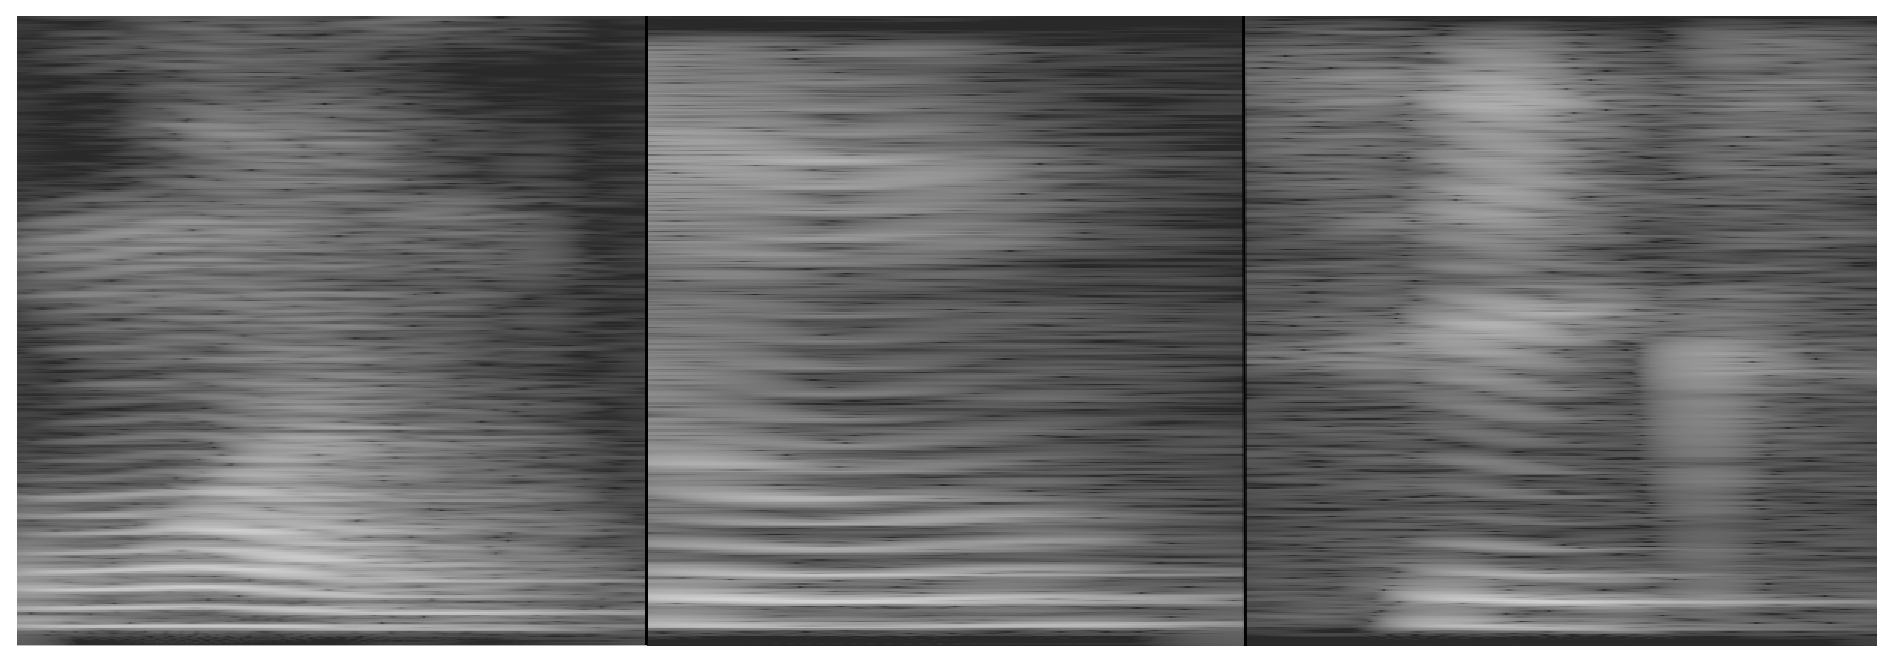
\includegraphics[scale=0.25]{specs}
	\caption{Spectrogram examples. Generated from audio files from the Free Spoken Digit Dataset \cite{fsdd}.}
	\label{fig:specs}
\end{figure}

\subsection{Fruit Classification}

This application classifies images of different types of fruits. The dataset is the Fruit Images Dataset \cite{fruit_ds}. This dataset contains a total of 90380 color images divided in 131 categories, where each category is a different kind of fruit. Each image is 100 by 100 pixels image. Figure \ref{fig:fruits} shows three examples of different fruit images from the dataset: blueberry, lime and strawberry.

\begin{figure}[thbp]
	\centering
	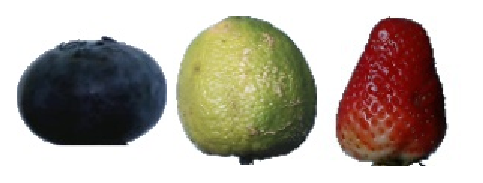
\includegraphics[scale=1.0]{fruits}
	\caption{Fruit examples. Taken from the Fruit Images Dataset \cite{fruit_ds}.}
	\label{fig:fruits}
\end{figure}

\subsection{Scene Classification}

These application classifies images of different natural scenes from around the world. The dataset is the Intel Image Classification \cite{intel_ds}. The dataset has 17034 color images of a size of 150 by 150 pixels. The categories are the following: buildings, forest, glacier, mountain, sea, street. Figure \ref{fig:scenes} shows three examples of different scene images from the dataset: buildings, mountain and sea.

\begin{figure}[thbp]
	\centering
	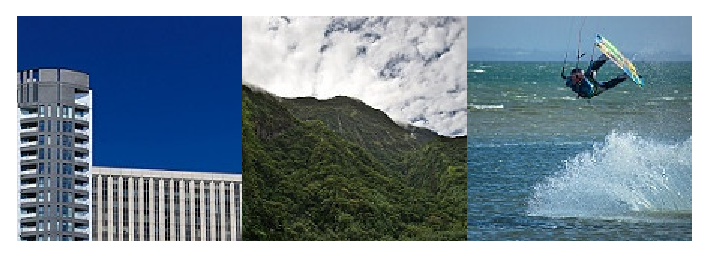
\includegraphics[scale=0.75]{scenes}
	\caption{Scenes examples. Taken from the Intel Image Classification Dataset \cite{intel_ds}.}
	\label{fig:scenes}
\end{figure}

\section{Neural Network Topologies}

Each application was trained on a different neural network, the amount of layers and the size and depth of these layers vary depending on the complexity of the application. Nonetheless, since all three applications are image classification problems they all follow a similar structure. The first layers are a convolutional layers combined with max pooling layers, which downsample the image. The pool size for all the pooling layers is 2 by 2 pixels, which means that the image is reduced to half the size. After that, there is a flattening layer which transforms the 2D image to a one-dimensional array. Finally, the network has a few dense (fully connected) layers. In the middle of the dense layers dropout layers can be inserted, which can help with overfitting. All the applications have a dropout rate of 0.25 which is a fairly typical value to use. All applications were trained for 50 epochs. The training parameters and the network topologies were chosen by trial and error in an iterative process where the parameters and topologies were refined until an optimal point was found where the size of the network was small enough and the accuracy was acceptable. Bigger network sizes had diminishing returns in accuracy for the audio and fruit classification problems. The scene classification problem still has room to improve in terms of accuracy, but for the purposes of this work an accuracy of more than 80\% was good enough and since it is the bigger network, training time was also a concern.
%Tables \ref{tab:audio_nn_topo}, \ref{tab:fruit_nn_topo} and \ref{tab:scene_nn_topo} show the topology for each of the different applications along with the total number of trainable parameters in the neural network. All applications were trained for 50 epochs.

\begin{table}[thbp]
\centering
\caption{Neural network topology for audio classification.}
\label{tab:audio_nn_topo}
\begin{tabular}{|l|l|}
\hline
\multicolumn{1}{|c|}{\textbf{Layer}}          & \multicolumn{1}{|c|}{\textbf{Details}}                     \\ \hline
Input          & shape=64x64x1               \\ \hline
Conv2D         & shape=64x64x32, kernel=3x3  \\ \hline
Conv2D         & shape=64x64x32, kernel=3x3  \\ \hline
MaxPooling2D   & pool\_size=2x2              \\ \hline
Conv2D         & shape=32x32x16, kernel=3x3  \\ \hline
Conv2D         & shape=32x32x16, kernel=3x3  \\ \hline
MaxPooling2D   & pool\_size=2x2              \\ \hline
Flatten        &                             \\ \hline
Dropout        & rate=0.25                   \\ \hline
Dense          & size=32                     \\ \hline
Dropout        & rate=0.25                   \\ \hline
Dense (Output) & size=10, activation=softmax \\ \hline
               &                             \\ \hline
\textit{Total params}   & 147,946                      \\ \hline
\end{tabular}
\end{table}

The audio network topology is shown in Figure \ref{tab:audio_nn_topo}. It consists of two consecutive convolutional layers of depth 32 followed by a pooling layer and another two consecutive convolutional layers of 3x3 kernels, this time with half the depth. After flattening the layers, there is one dense layer before the final output layer.

\begin{table}[thbp]
\centering
\caption{Neural network topology for fruit classification.}
\label{tab:fruit_nn_topo}
\begin{tabular}{|l|l|}
\hline
\multicolumn{1}{|c|}{\textbf{Layer}}          & \multicolumn{1}{|c|}{\textbf{Details}}                     \\ \hline
Input          & shape=100x100x3              \\ \hline
Conv2D         & shape=100x100x48, kernel=5x5 \\ \hline
MaxPooling2D   & pool\_size=2x2               \\ \hline
Conv2D         & shape=50x50x32, kernel=5x5   \\ \hline
MaxPooling2D   & pool\_size=2x2               \\ \hline
Conv2D         & shape=12x12x24, kernel=5x5   \\ \hline
MaxPooling2D   & pool\_size=2x2               \\ \hline
Flatten        &                              \\ \hline
Dropout        & rate=0.25                    \\ \hline
Dense          & size=128                     \\ \hline
Dropout        & rate=0.25                    \\ \hline
Dense          & size=64                      \\ \hline
Dropout        & rate=0.25                    \\ \hline
Dense (Output) & size=131, activation=softmax \\ \hline
               &                              \\ \hline
\textit{Total params}   & 520,571                       \\ \hline
\end{tabular}
\end{table}

The fruit classification topology shown in Figure \ref{tab:fruit_nn_topo} uses a different approach. This time the kernels is of size 5x5 and there is a pooling layer between each convolutional layer. The depth of the convolutional layers is reduced decrementally in each stage. This time there are two dense layers before the final output layer, which size is bigger than the audio layer to accommodate for more categories in the dataset.

\begin{table}[thbp]
\centering
\caption{Neural network topology for scene classification.}
\label{tab:scene_nn_topo}
\begin{tabular}{|l|l|}
\hline
\multicolumn{1}{|c|}{\textbf{Layer}}          & \multicolumn{1}{|c|}{\textbf{Details}}                     \\ \hline
Input          & shape=150x150x3              \\ \hline
Conv2D         & shape=150x150x48, kernel=5x5 \\ \hline
Conv2D         & shape=150x150x48, kernel=3x3 \\ \hline
MaxPooling2D   & pool\_size=2x2               \\ \hline
Conv2D         & shape=75x75x32, kernel=5x5   \\ \hline
Conv2D         & shape=75x75x32, kernel=3x3   \\ \hline
MaxPooling2D   & pool\_size=2x2               \\ \hline
Conv2D         & shape=37x37x24, kernel=5x5   \\ \hline
Conv2D         & shape=37x37x24, kernel=3x3   \\ \hline
MaxPooling2D   & pool\_size=2x2               \\ \hline
Flatten        &                              \\ \hline
Dropout        & rate=0.25                    \\ \hline
Dense          & size=256                     \\ \hline
Dropout        & rate=0.25                    \\ \hline
Dense          & size=128                     \\ \hline
Dropout        & rate=0.25                    \\ \hline
Dense          & size=64                      \\ \hline
Dropout        & rate=0.25                    \\ \hline
Dense (Output) & size=6, activation=softmax   \\ \hline
               &                              \\ \hline
\textit{Total params}   & 2,128,998                      \\ \hline
\end{tabular}
\end{table}

The scene classification application dataset has the most complex images and it uses the bigger of the neural networks, with a total of six convolutional layers, three dense layers before the output layer. In total, the layer has more than 2 million trainable parameters.

\section{Optimizations}

With the objective of improving the performance of the selected applications the following optimizations were tested.

\begin{itemize}
    \item \textbf{Reduced input size.} Reducing the size of the images can reduce the amount of detail in the image and reduce the accuracy of the neural network since now it does not have enough detail to work with. On the other side, applying convolutions through smaller images can accelerate the inference process. On top of this, when using the Myriad X VPU in the NCS2 there is less data that needs to travel through the USB3 bus to the accelerator.
    \item \textbf{Reduced CNN depth and layer size.} One of the main parameters that can be modified when defining the neural network is how much depth the CNN has. More depth means that the neural network can identify more features in an image. Reducing the depth will limit that capacity but on the other hand it will make the network faster since there are less calculations to make.
    \item \textbf{Pruning.} This technique sets some of weights of the neural network to zero. If the hardware has support for this, it means that it can skip some multiplications, since the result is are zero anyways.
    \item \textbf{Separable Convolution}. This method uses a different layer which separates the normal convolution into two steps: a depth-wise convolution and a point-wise convolution (see Chapter 2, Section 2.1.3). This reduces the number of operations that need to be done and the amount of trainable parameters that the network has. Since the number of parameters is lower, the network can be harder to train and the accuracy can drop.
\end{itemize}

\section{Measurements}

All the experiments and measurements were performed using a Raspberry Pi 4 Model B. For the same neural network two different versions were run. The first one will run with Tensorflow directly in the Raspberry Pi CPU. The second one is an OpenVINO optimized version running in the NCS2 attached to one of the USB3 ports. All tests were done using Tensorflow 1.15 and OpenVINO 2020.1.

\begin{figure}[thbp]
	\centering
	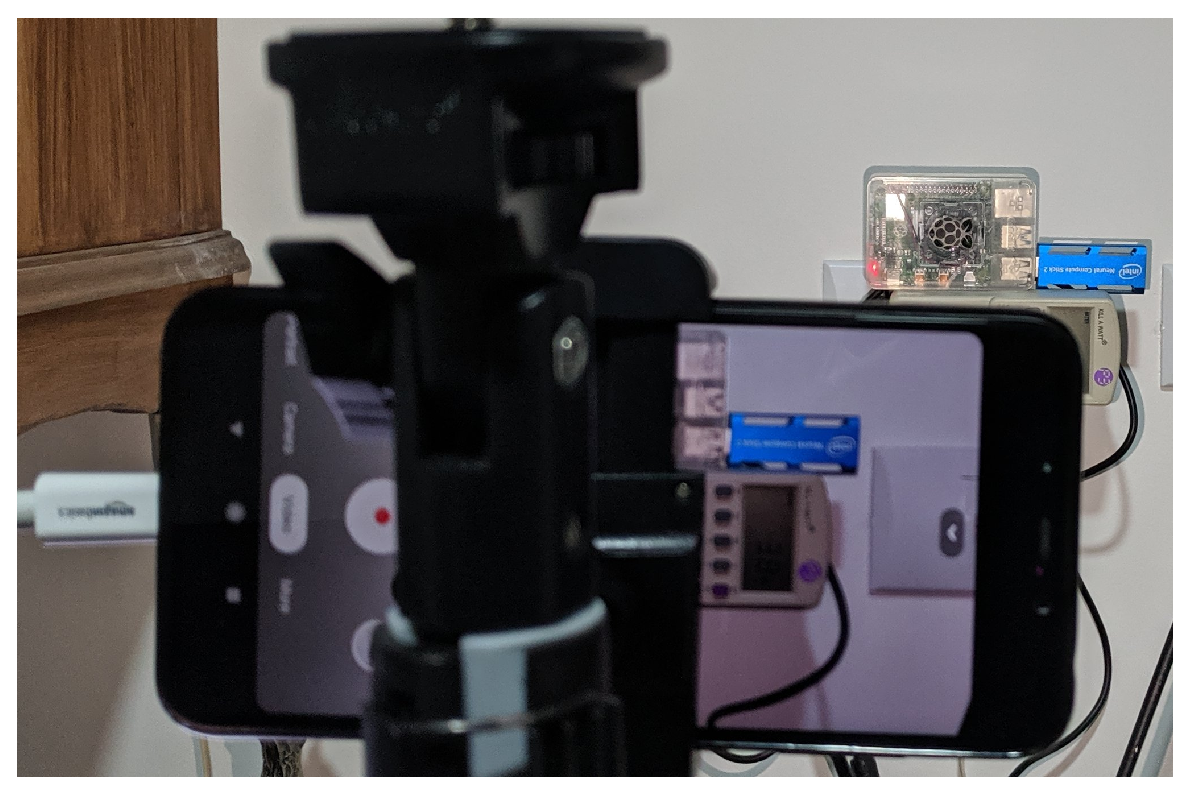
\includegraphics[scale=0.15]{setup2}
	\caption{Test platform. Raspberry Pi 4 with NCS2 attached. Cell phone camera recording power consumption.}
	\label{fig:setup2}
\end{figure}

For each of the three applications these three measurements are considered:

\begin{itemize}
    \item \textbf{Accuracy.} The test dataset is used to test the accuracy of the network. It is given by the percentage of correctly predicted classes out of the total images.
    \item \textbf{Performance.} This is measured doing inference on the whole test dataset and measuring how much time it takes to do the inference. Then, the number of images in the dataset is divided by the amount of time it took to run and that gives the performance metric with units of inferences per second.
    \item \textbf{Average power consumption.} This is measured in Watts and is measured using a Kill-A-Watt device attached to the power brick that powers the device under test (see Figure \ref{fig:setup2}). This measures the complete system power. Note: The NCS2 consumes power when idle, so when measurements were done using Tensorflow the NCS2 was removed from the Raspberry Pi.
\end{itemize}

Apart from these, a fourth, derived metric, is going to be analyzed and it is the \textbf{energy efficiency} measured as performance per Watt. This can be obtained by simply dividing the performance metric by the power consumption (see Equation \ref{eq:ee}).

\begin{equation}\label{eq:ee}
EE = Pe / PC
\qquad (inferences/s/Watt)
\end{equation}

All the mentioned measurements were performed for all the techniques mentioned in the optimizations section above. On top of that, two extra sets of measurements were done: one where all the techniques are combined and another where all the techniques, except for separable convolution, were combined. The reduced input size will reduce the image by 25\%. The reduced CNN depth and layer size will reduce the depth of all the CNNs by 25\% and the amount of neurons in all the fully connected layers by 25\%. For the pruning optimization a pruning target of 50\% is used.

\section{Experimental Evaluation}

\subsection{Accuracy}

Figures \ref{fig:acc-audio}, \ref{fig:acc-fruit} and \ref{fig:acc-scene} show the accuracy achieved by the trained neural networks. These results were measured using the corresponding test dataset. The accuracy was the same for both Tensorflow and OpenVINO.

\begin{figure}[thbp]
	\centering
	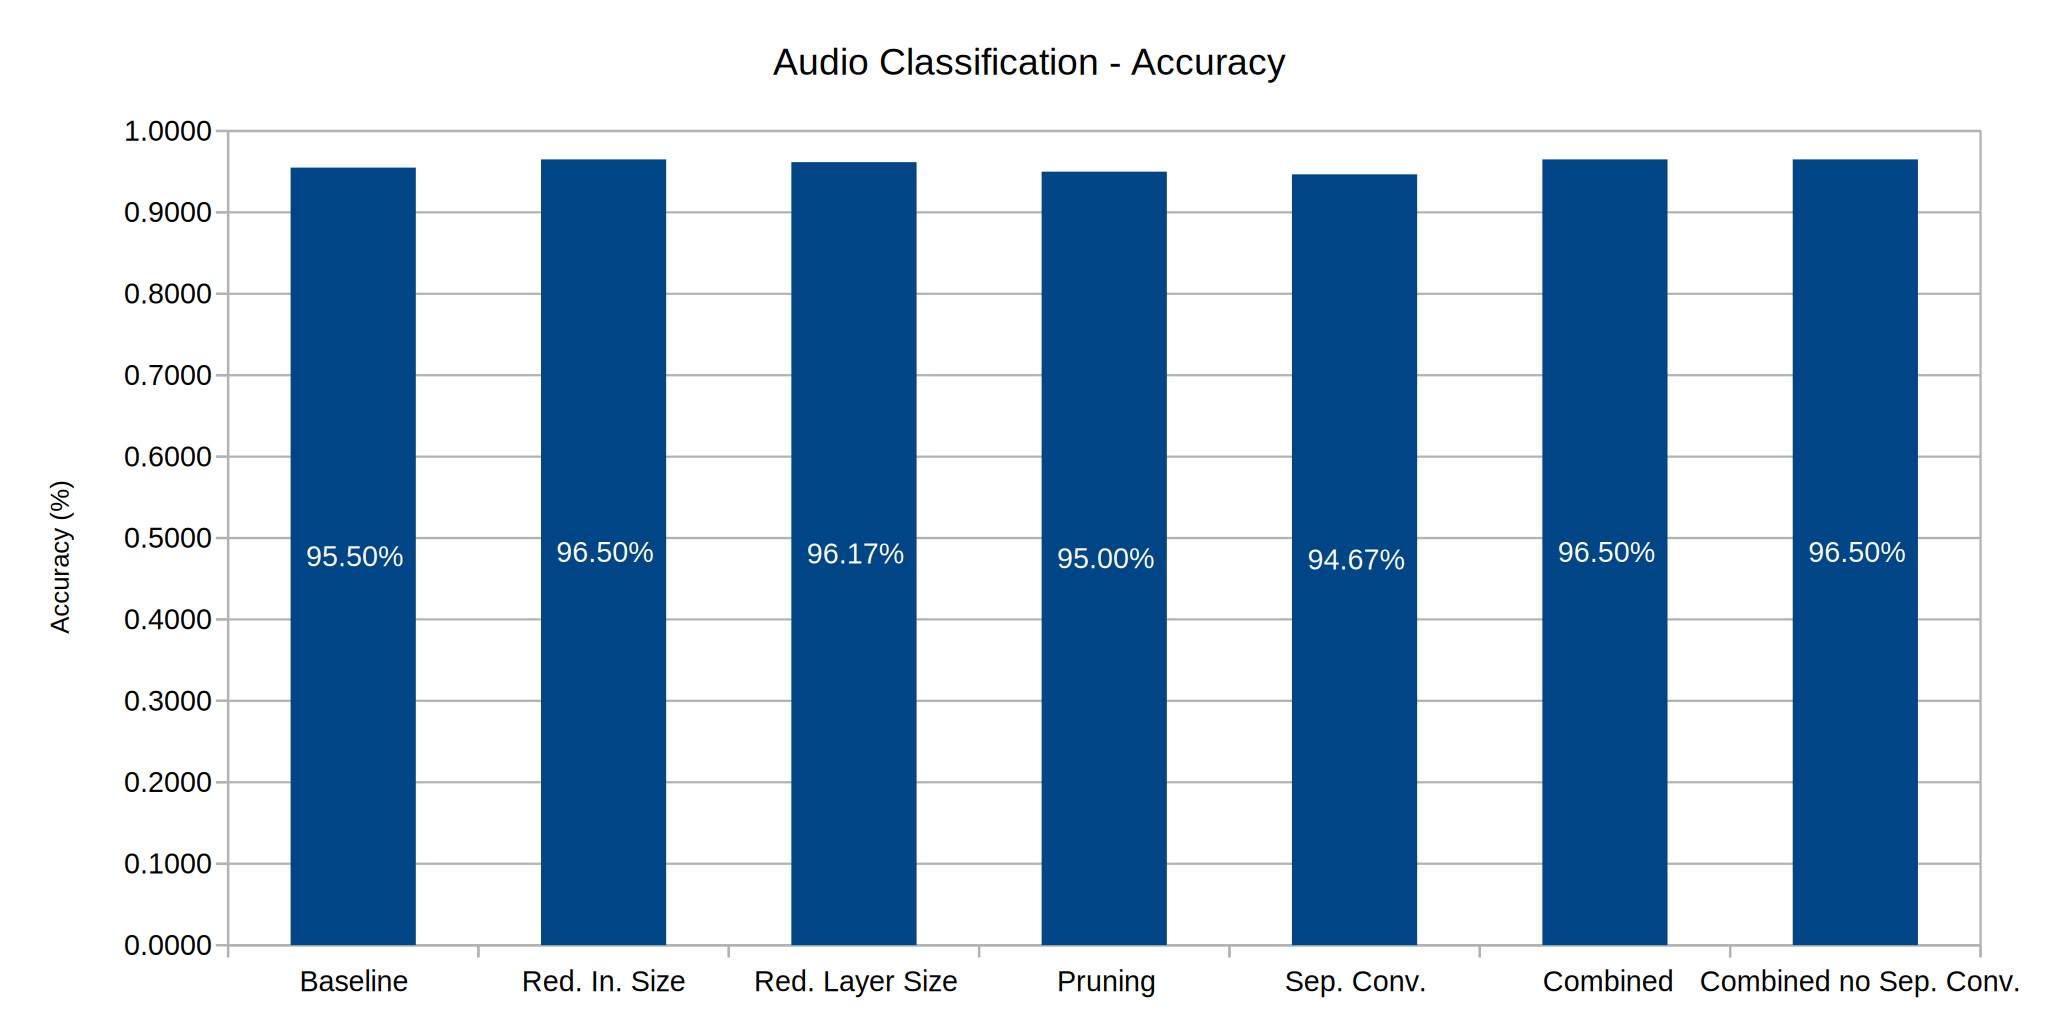
\includegraphics[scale=0.65]{acc-audio}
	\caption{Audio classification: accuracy comparison.}
	\label{fig:acc-audio}
\end{figure}

For the audio classification app the accuracy remains fairly consistent across the different optimizations. Compared to the baseline the worst degradation was seen when running the separable convolution, which reduced the accuracy by 0.83\%. The best case improved the accuracy by 1\%, in the case of the reduced input size and both optimizations with combined techniques.

\begin{figure}[thbp]
	\centering
	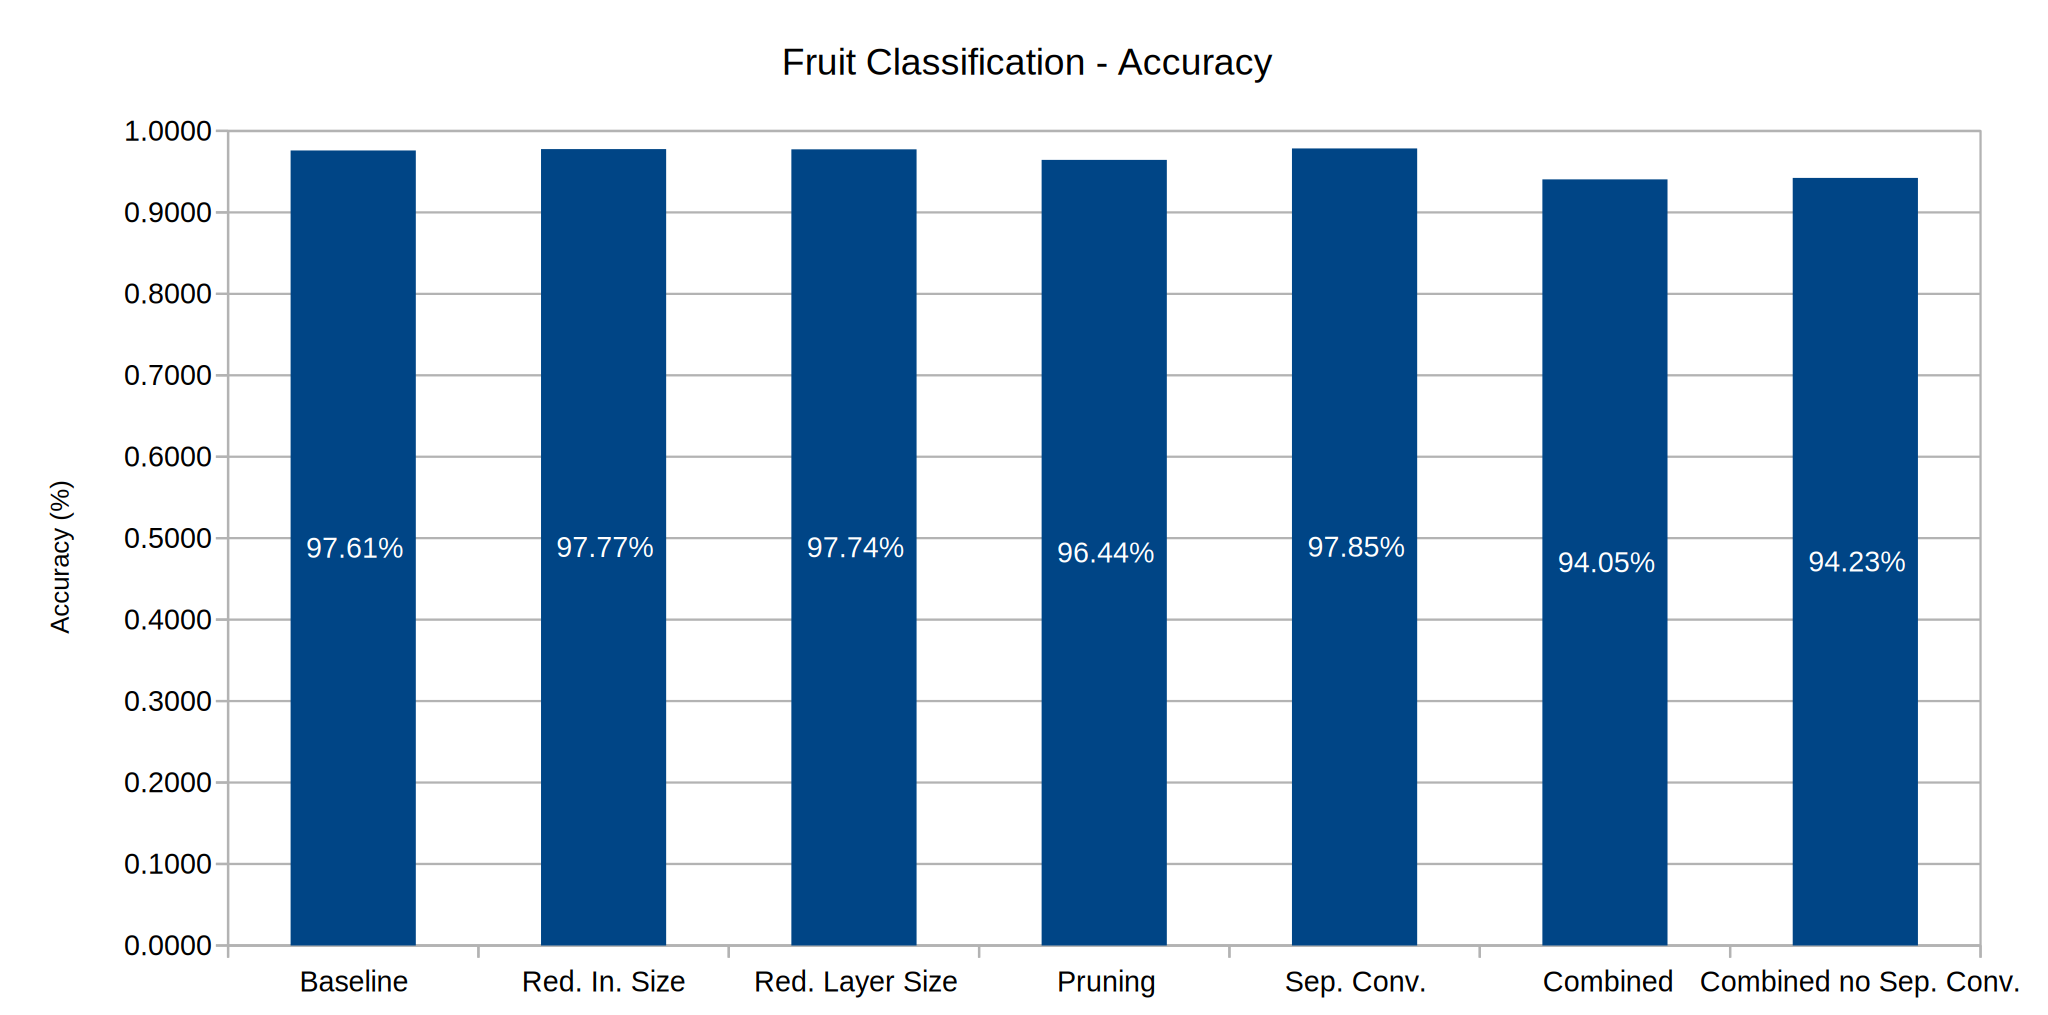
\includegraphics[scale=0.65]{acc-fruit}
	\caption{Fruit classification: accuracy comparison.}
	\label{fig:acc-fruit}
\end{figure}

In the case of the fruit classification the optimization techniques individually didn't have a significant impact in the accuracy. However when combining several techniques together there is a measurable decline in the accuracy. At 94.04\% the accuracy fell by 3.56\%.

\begin{figure}[thbp]
	\centering
	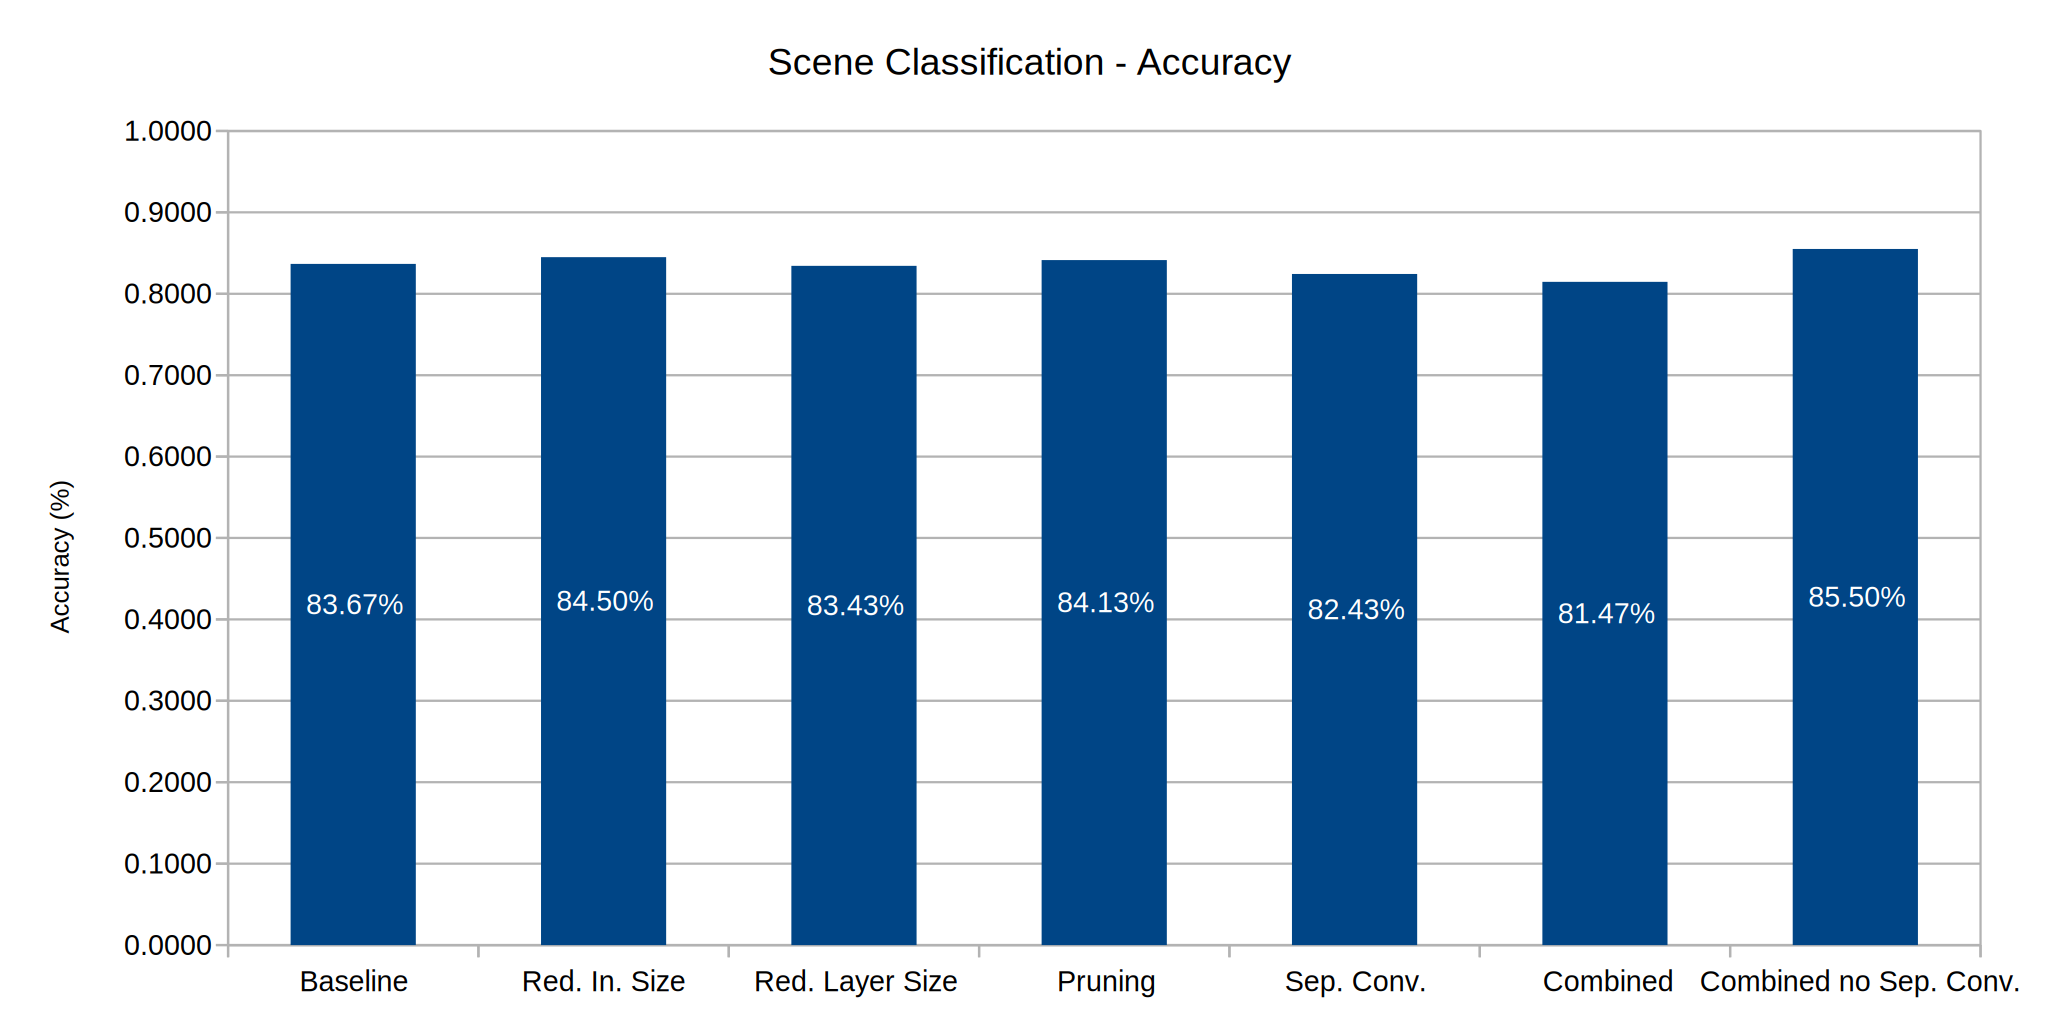
\includegraphics[scale=0.65]{acc-scene}
	\caption{Scene classification: accuracy comparison.}
	\label{fig:acc-scene}
\end{figure}

The scene classification application shows a similar behaviour as the audio classification application. No clear trend is set, which means that the optimization does not really affect the accuracy in a significant way. In fact, when combining all methods except for the separable convolution the accuracy actually improved 1.83\%.

In general, it can be seen that the accuracy is not degraded for the audio and scene classification applications even when combining all the optimizations. The only case where a clear conclusion can be made is in the fruit classification application where the combination of techniques hurts the accuracy by a small percentage.

\subsection{Performance}

Figures \ref{fig:acc-audio}, \ref{fig:acc-fruit} and \ref{fig:acc-scene} show the performance for each of the optimization techniques for both Tensorflow and OpenVINO.

\begin{figure}[thbp]
	\centering
	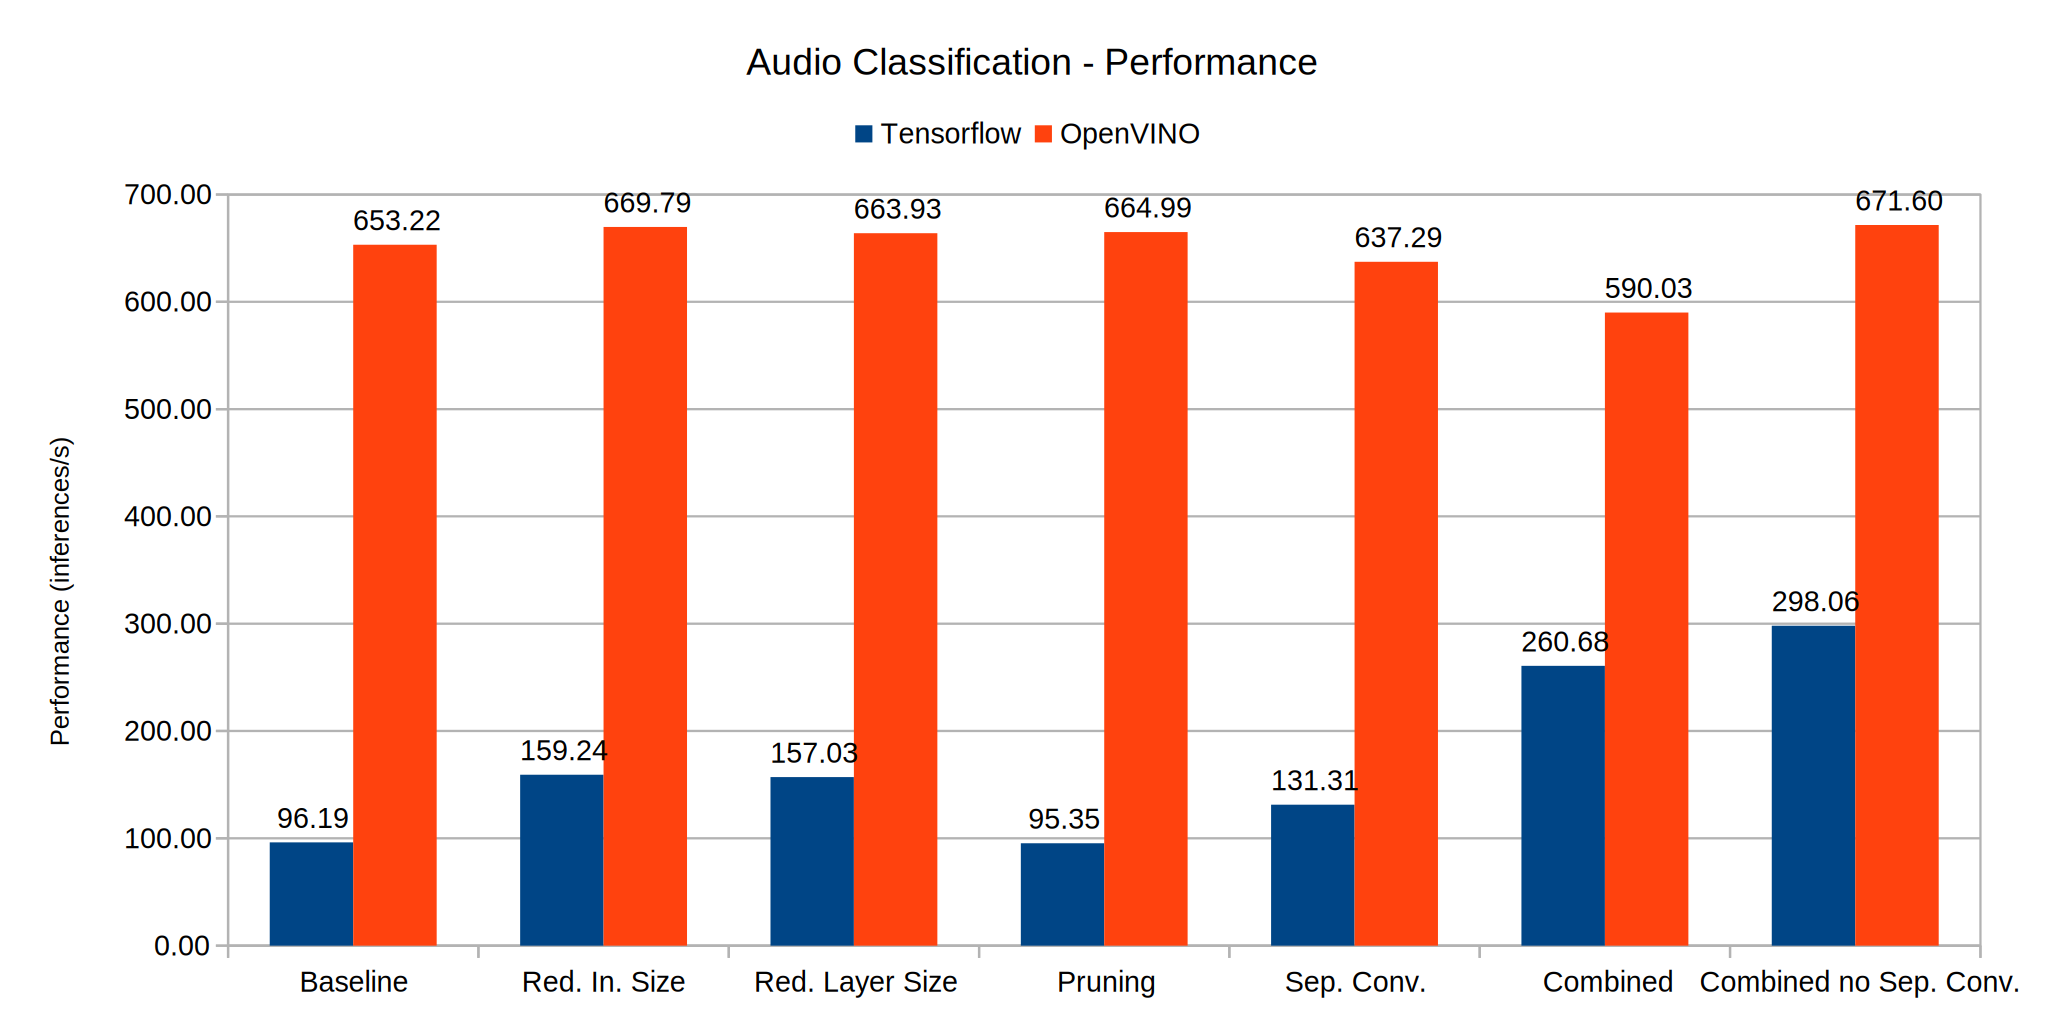
\includegraphics[scale=0.65]{perf-audio}
	\caption{Audio classification: performance comparison.}
	\label{fig:perf-audio}
\end{figure}

Looking at the Tensorflow results for the audio classification application in Figure \ref{fig:acc-audio} all the optimizations except for pruning improved the performance. The best case scenario was achieved by combining all the optimizations except the separable convolution. For that best case the performance improved by 209.9\%. In the case of OpenVINO the best case was also the combined without separable convolution. The difference is that in this case the performance gain was minimal, only an improvement of 2.8\%. Another notable result is that the separable convolution actually hurts performance in this application. In this application OpenVINO was faster than Tensorflow by 125.3\% when comparing the best result for each.

\begin{figure}[thbp]
	\centering
	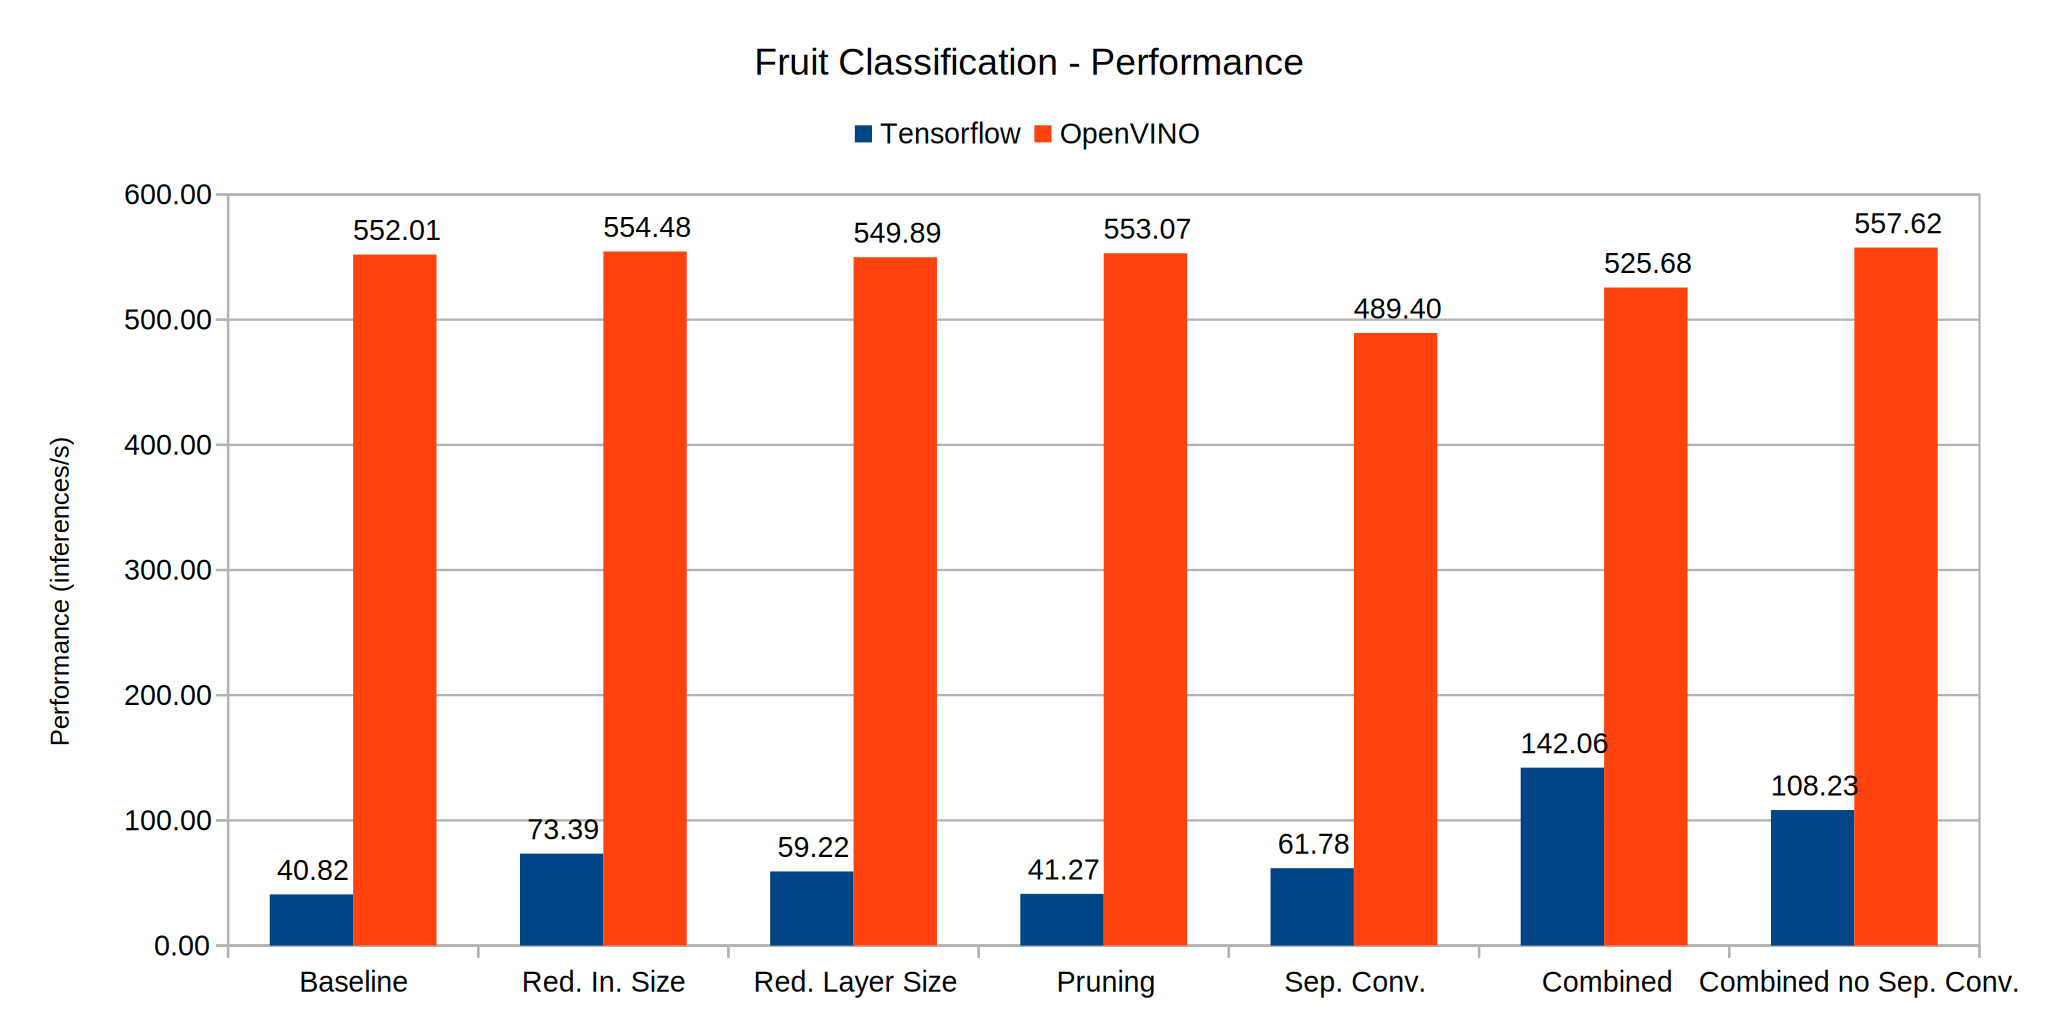
\includegraphics[scale=0.65]{perf-fruit}
	\caption{Fruit classification: performance comparison.}
	\label{fig:perf-fruit}
\end{figure}

The fruit classification application follows a similar trend to the audio classification application (see Figure \ref{fig:acc-fruit}). In this case the difference is that in Tensorflow combining all techniques gives the best performance improvement, which is of 248\%. OpenVINO's trend is the same as for the audio application, where the separable convolution hurts performance so combining all techniques except for it gives the best result. This improvement is very small though, just a 1\%. When the best case for Tensorflow and OpenVINO is compared, it can be seen that OpenVINO is faster by 292.5\%.

\begin{figure}[thbp]
	\centering
	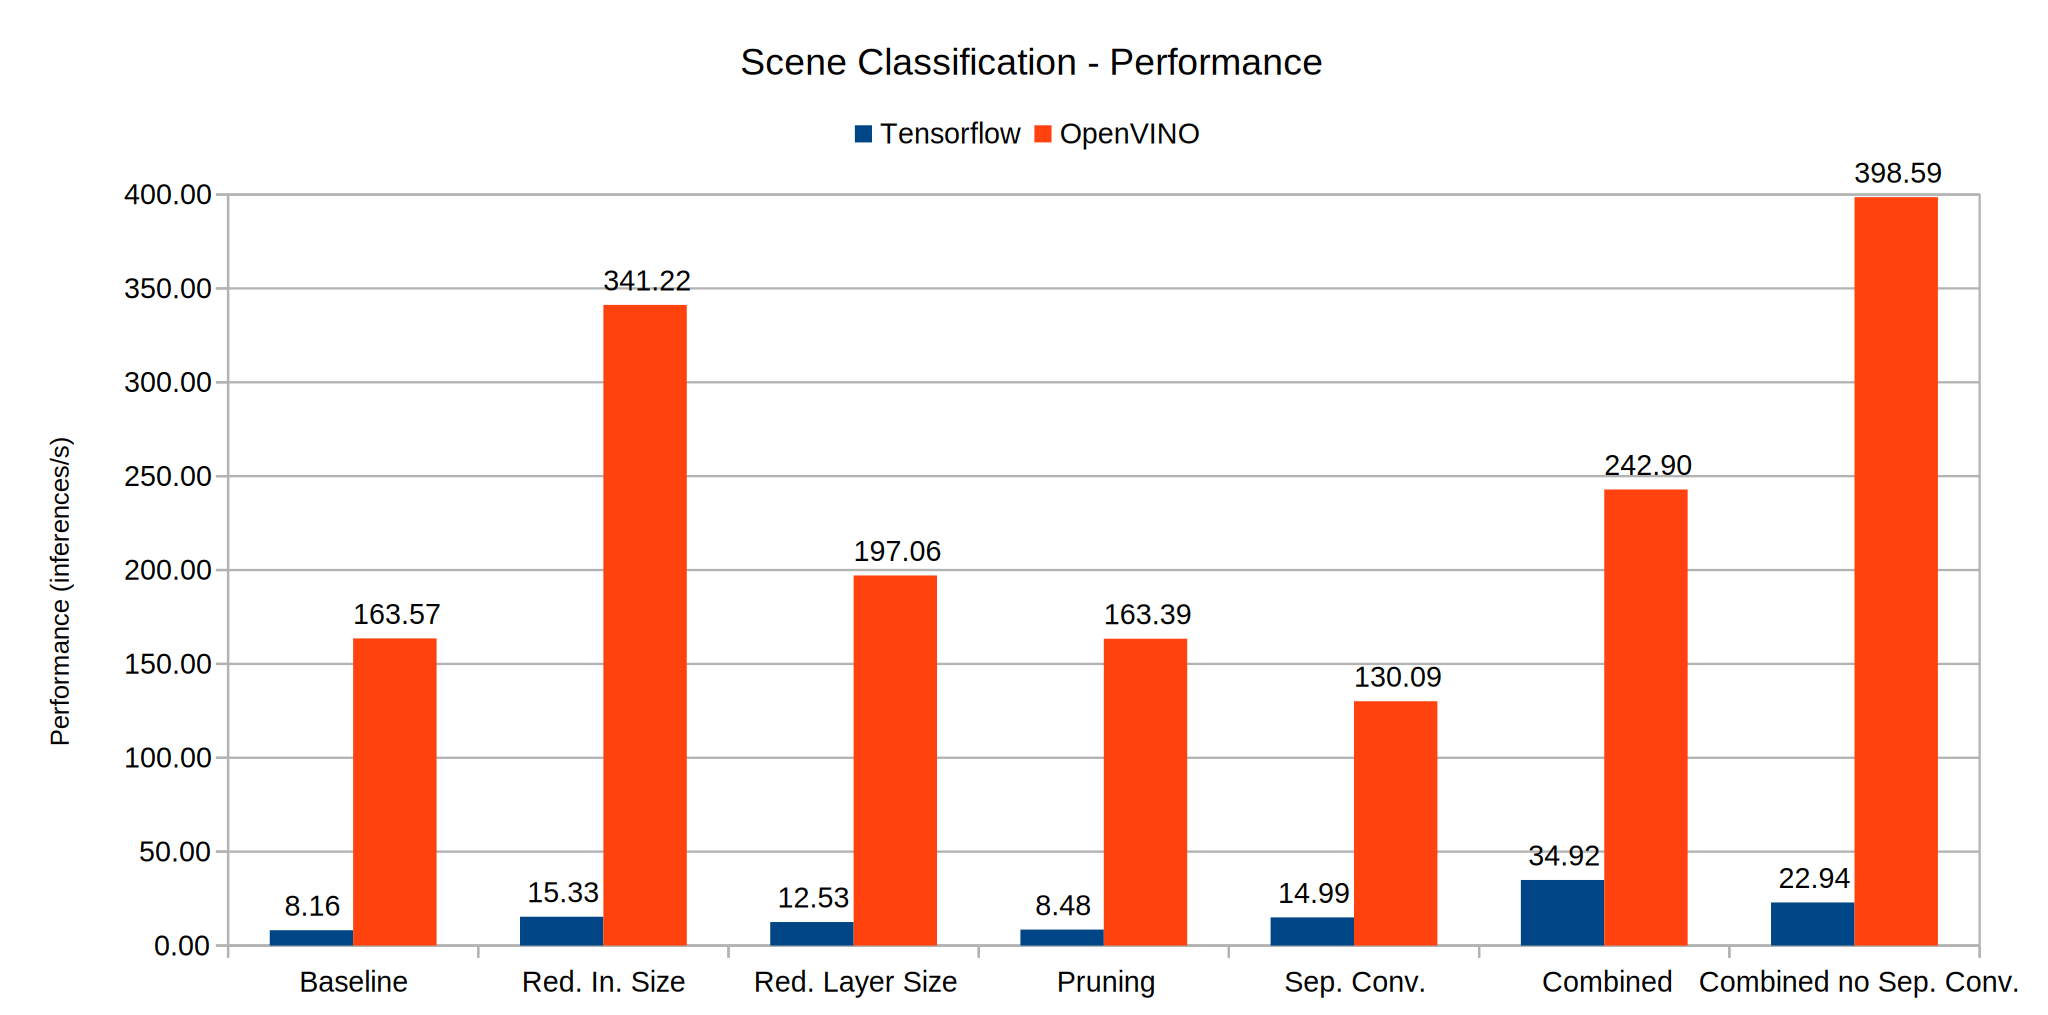
\includegraphics[scale=0.65]{perf-scene}
	\caption{Scene classification: performance comparison.}
	\label{fig:perf-scene}
\end{figure}

In the scene classification application using Tensorflow (see Figure \ref{fig:acc-scene}) the best case achieved was combining all the optimizations, this improved the performance by 328\%. For the case of OpenVINO, this is the only application where a significant improvement can be seen when optimizing the neural network. The best case was again the combination of techniques except for the separable convolution, but this time the improvement was 143.7\%. This application presents the most extreme improvement when comparing Tensorflow and OpenVINO. This time the difference is of 1041.4\%.

This classification problem clearly has a different trend from the other two, the optimizations techniques had a much greater impact on the results. This is the more complex application and as such utilizes a bigger neural network with more than 2 million parameters, compared to 500,000 and 150,000 of the other applications. This means that the Myriad X accelerator spends more of its time doing calculations to execute the network and is not bottle-necked by the data transfer from and to the NCS2. The neural networks of the first two applications are too small and execute so fast that the real impact of the optimization techniques cannot be seen because there are other bottle-necks in the system that hide the optimizations.

In general, a clear trend can be seen where Tensorflow can get significant performance improvements when applying the optimizations but with OpenVINO it varies greatly depending on the application. Another clear result is that the separable convolution optimization doesn't work well with OpenVINO and the NCS2 to the point where it actually hurts performance. In contrast the separable convolution did help when running the applications with Tensorflow. When comparing Tensorflow with respect to OpenVINO it is clear that significant gains in performance can be obtained when running the neural networks in a specialized accelerator such as the Myriad X VPU, applications can run up to 10 times faster when using an optimized toolkit and hardware. The only optimization that didn't affect the results was pruning. This indicates that neither Tensorflow nor OpenVINO are optimized to take advantage of this technique and it is not worth using it.

\subsection{Accuracy vs Performance}

In this section a comparison is made between the accuracy and the performance of the different optimizations. The best results are the ones towards the top right corner, where both the accuracy and performance are maximized. Note that even though the difference between the worst and best case may be small, the graphs are zoomed to fit the data and the difference may seem bigger than they are. This is shown for the OpenVINO scenario.

\begin{figure}[thbp]
	\centering
	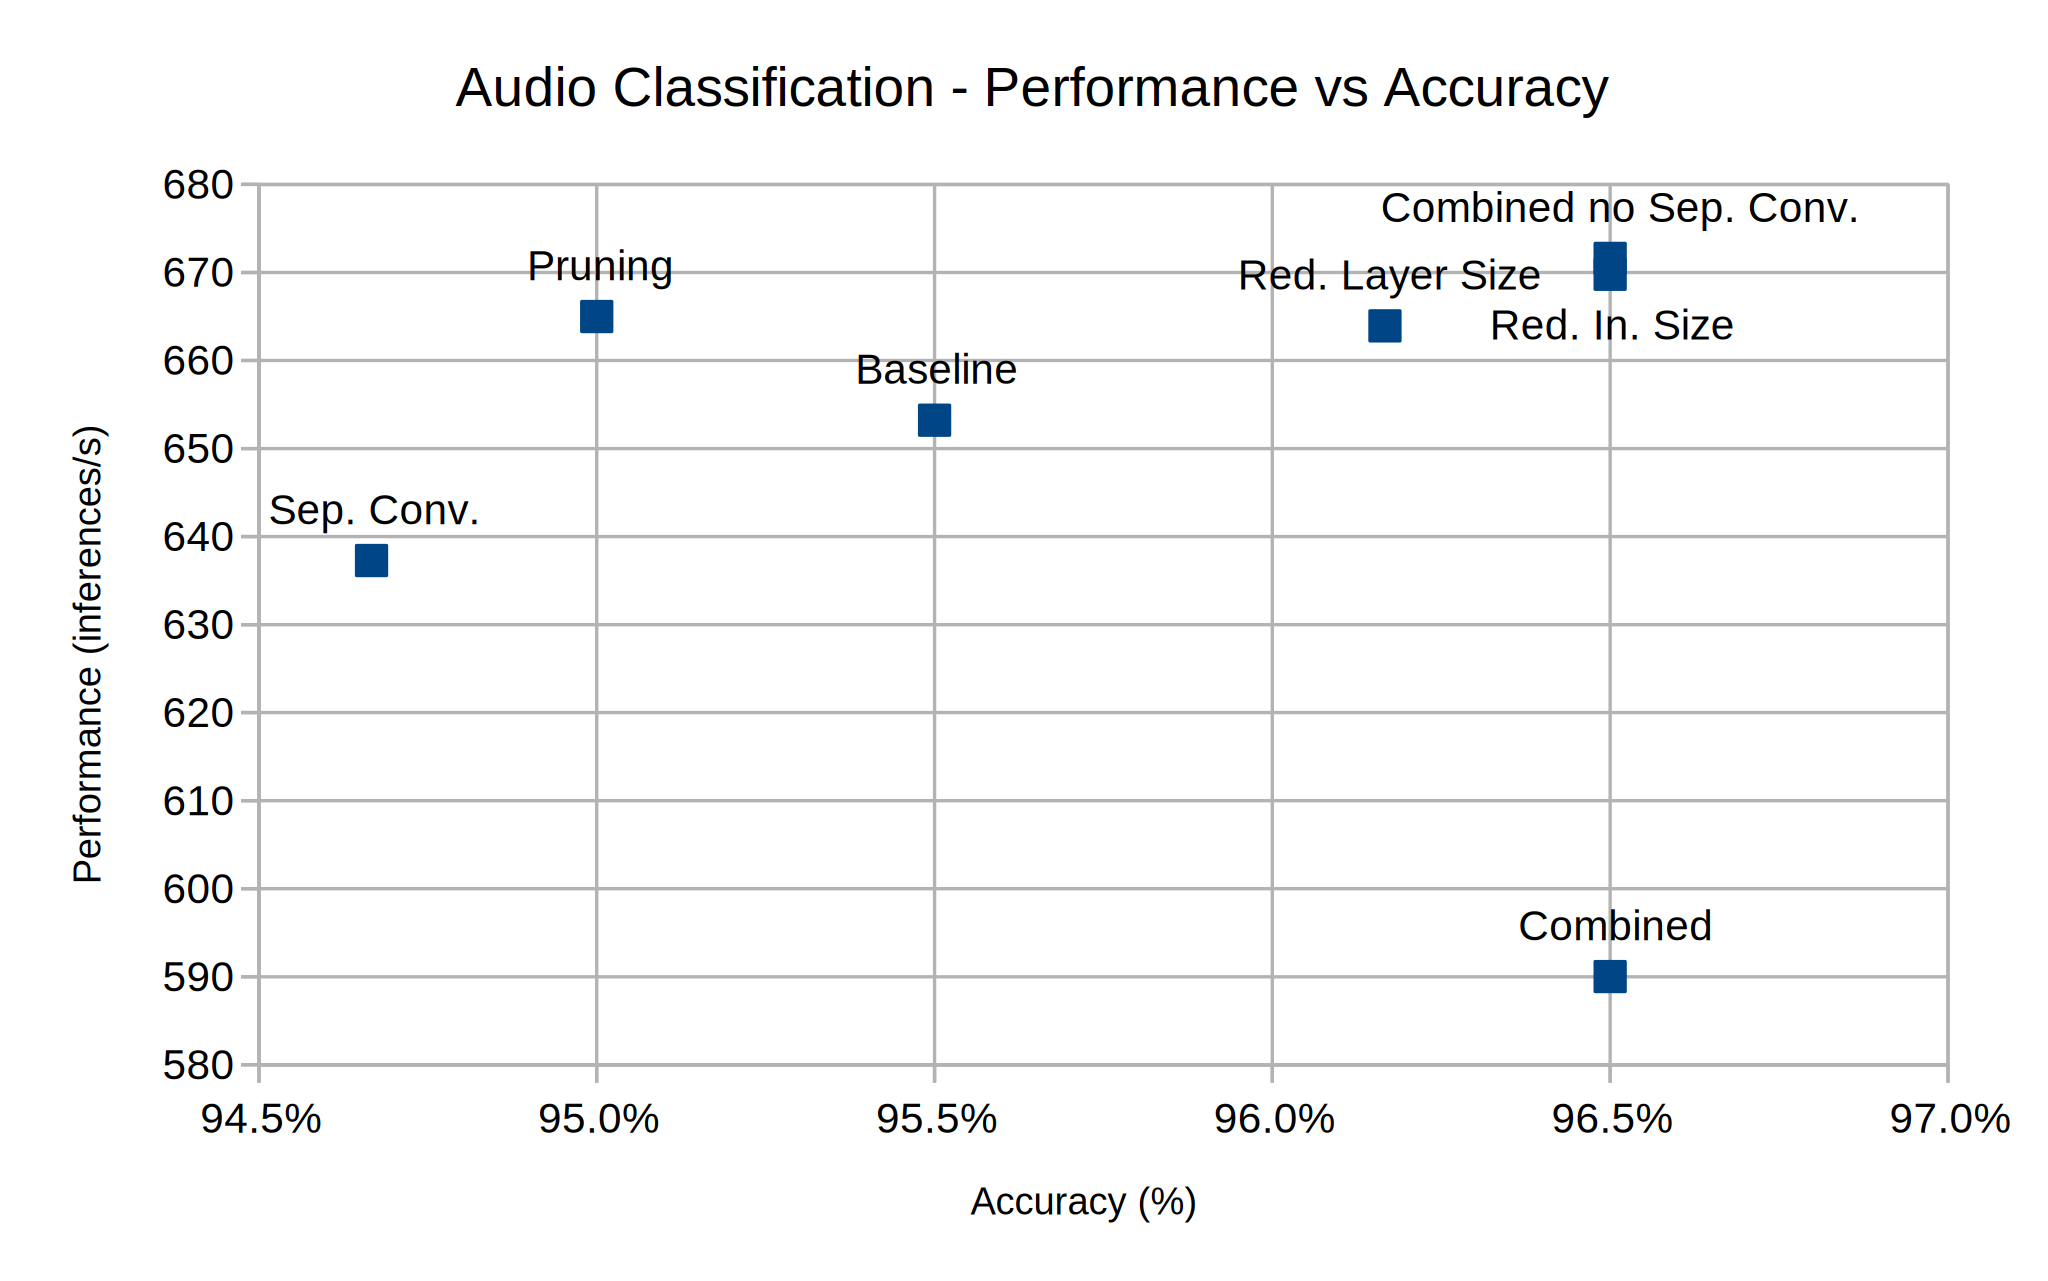
\includegraphics[scale=0.75]{vs-audio}
	\caption{Audio classification: accuracy vs performance.}
	\label{fig:vs-audio}
\end{figure}

In Figure \ref{fig:vs-audio} the results from the audio classification application are shown. The clear winners here are the reduce input size optimization and the case where all optimizations except for the separable convolution are applied. Both have an accuracy of 96.5\% and the performance is nearly identical. This means that reducing the input size of the image is enough optimization to improve the performance without hurting the accuracy.

\begin{figure}[thbp]
	\centering
	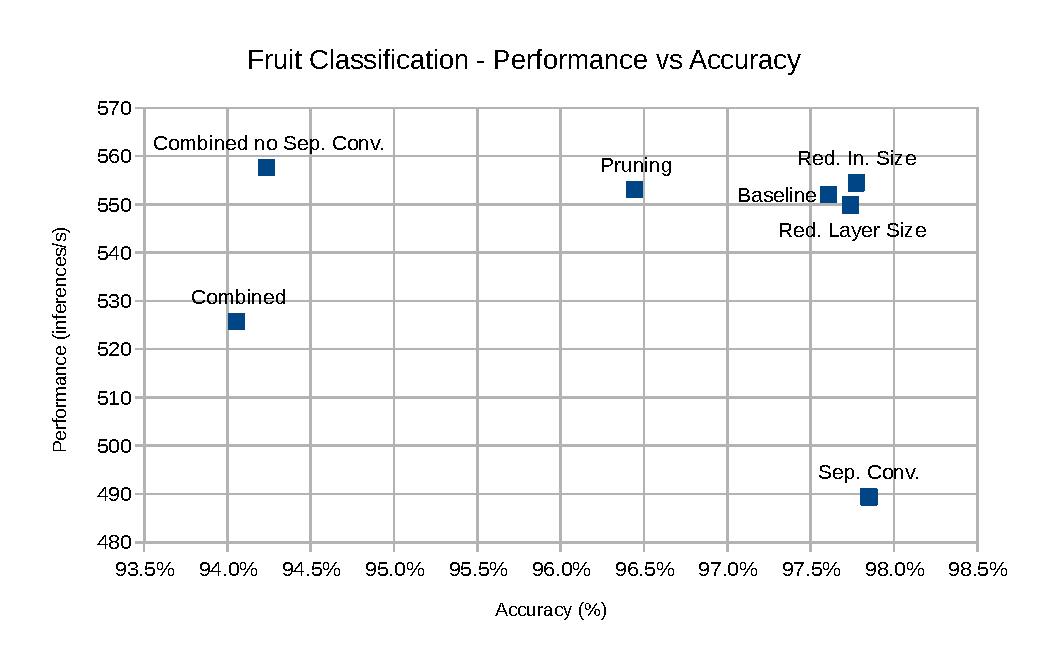
\includegraphics[scale=0.75]{vs-fruit}
	\caption{Fruit classification: accuracy vs performance.}
	\label{fig:vs-fruit}
\end{figure}

Figure \ref{fig:vs-fruit} shows the results for the fruit classification application. For this application the performance improvements are minimal, the best results range between 550 to 560 inferences per second. In this case there are three results clustered in the top right corner. Since the difference between them is so small running the optimizations in this application is almost insignificant when running it in OpenVINO and the baseline application can be run without losing performance or accuracy.

\begin{figure}[thbp]
	\centering
	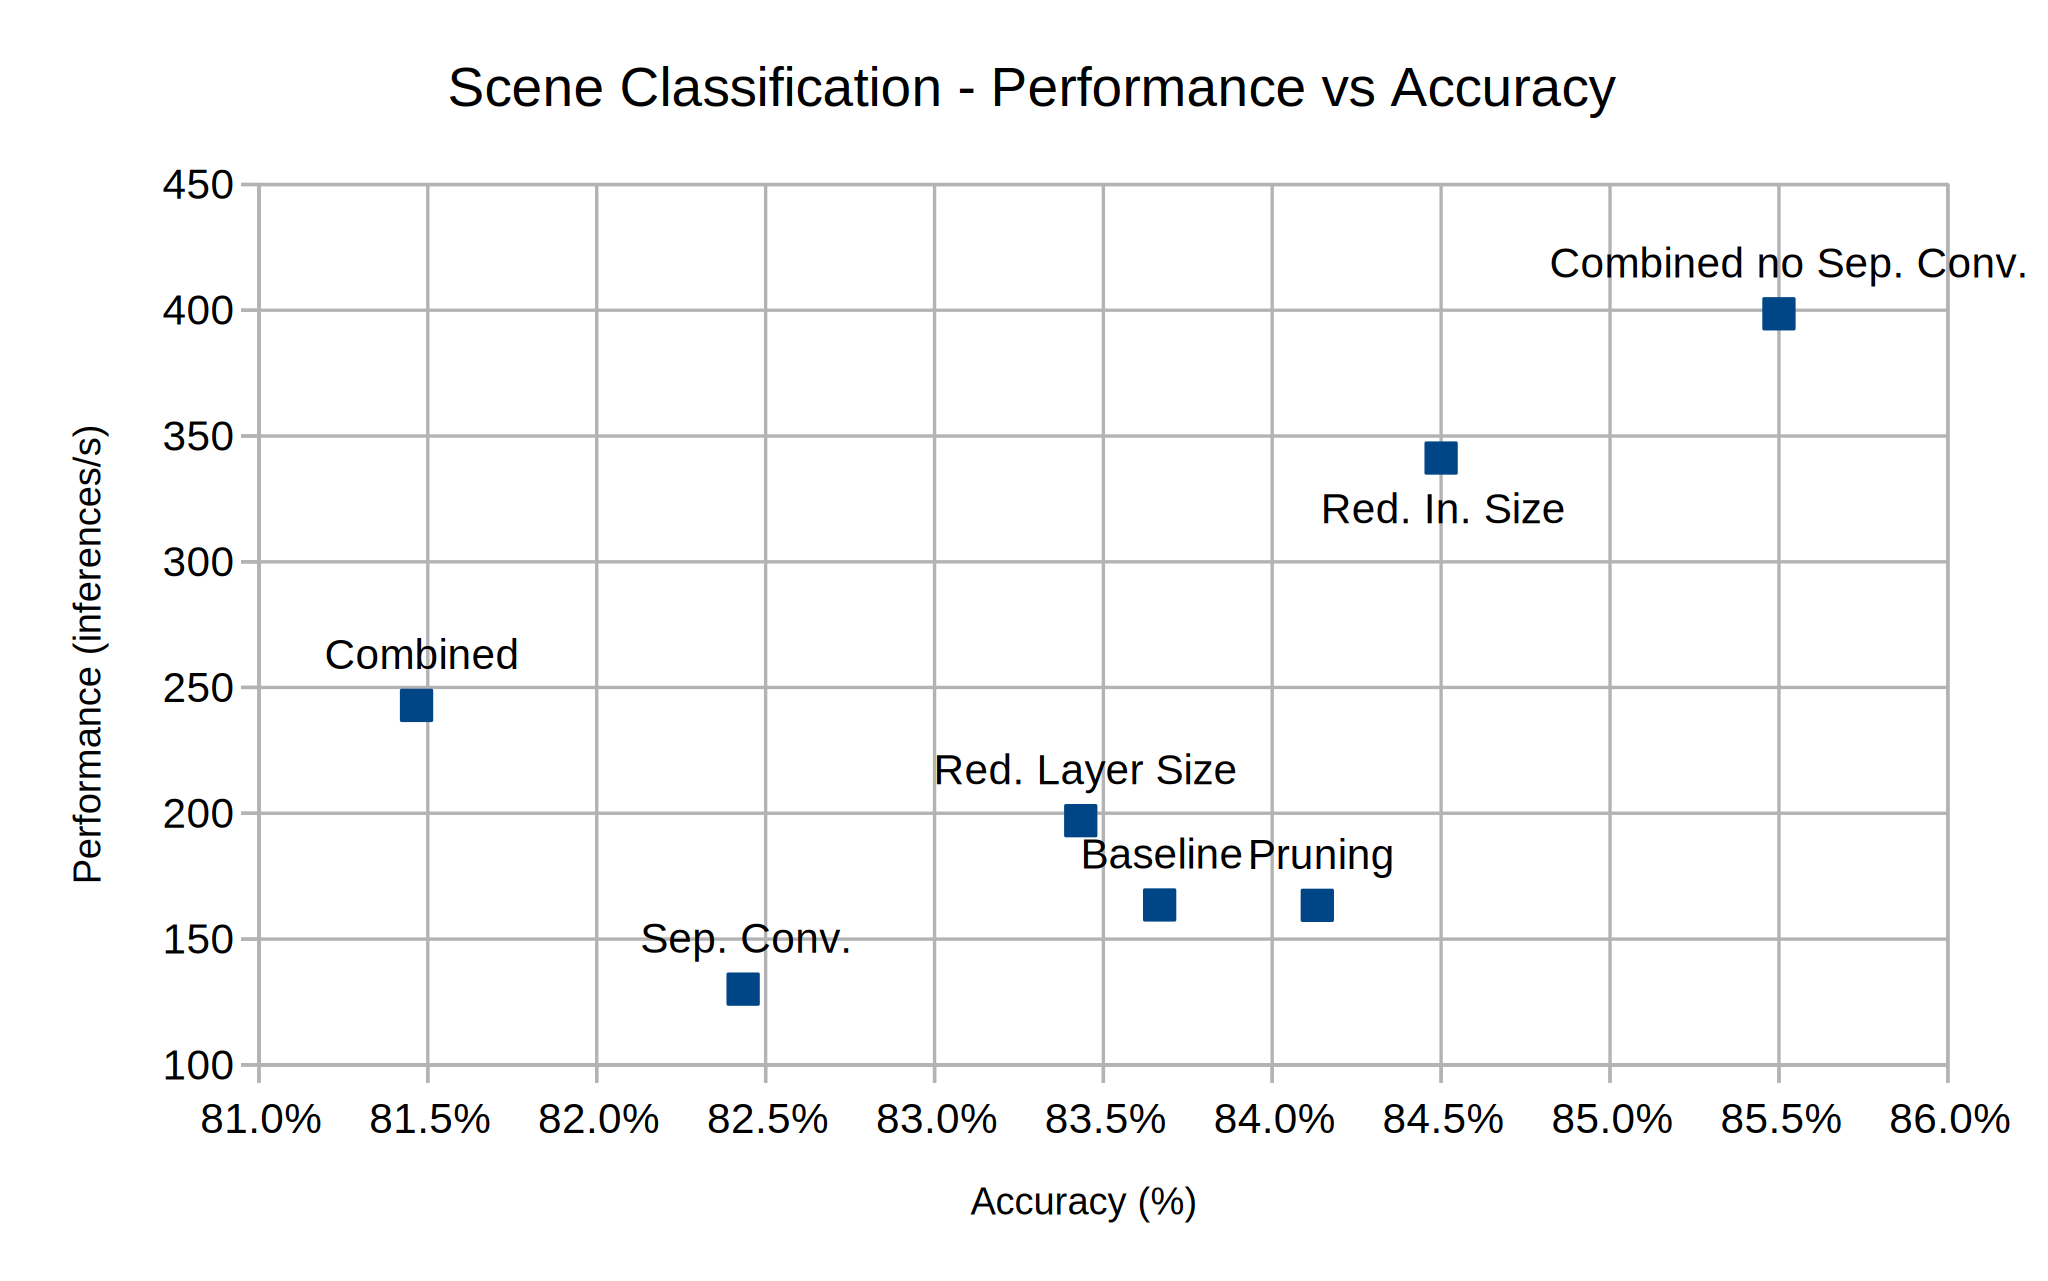
\includegraphics[scale=0.75]{vs-scene}
	\caption{Scene classification: accuracy vs performance.}
	\label{fig:vs-scene}
\end{figure}

For the scene classification application (shown in Figure \ref{fig:vs-scene}) there is a clear winner: combining all the optimization except for the separable convolution. Not only does it have the best performance, it also has the best accuracy. This time the performance is significant (2.43 times faster) unlike the other applications where the performance difference was almost insignificant, only improving by 1 to 3 percent.

\subsection{Power Consumption and Energy Efficiency}

When each of the applications were running the power consumption was logged and a final metric of the average power consumption was calculated, this is measured in Watts. The energy efficiency is defined as the performance per Watt, this is calculated by dividing the performance by the average power consumption.

\begin{table}[thbp]
\centering
\caption{Average power consumption for the audio classification application.}
\label{tab:eet-audio}
\begin{tabular}{|l|l|l|}
\hline
\multicolumn{1}{|c|}{\multirow{2}{*}{\textbf{Optimization}}} & \multicolumn{2}{c|}{\textbf{Power (W)}}                                           \\ \cline{2-3} 
\multicolumn{1}{|c|}{}                                       & \multicolumn{1}{c|}{\textbf{Tensorflow}} & \multicolumn{1}{c|}{\textbf{OpenVINO}} \\ \hline
Baseline                                                     & 5.9                 & 6.2               \\ \hline
Reduced Input Size                                           & 6.0                 & 6.0               \\ \hline
Reduced Layers Size                                          & 6.1                 & 6.1               \\ \hline
Pruning                                                      & 5.9                 & 6.1               \\ \hline
Separable Convolution                                        & 5.4                 & 6.2               \\ \hline
Combined                                                     & 5.0                 & 5.9               \\ \hline
Combined without Separable Convolution                       & 5.9                 & 6.0               \\ \hline
\end{tabular}
\end{table}

\begin{figure}[thbp]
	\centering
	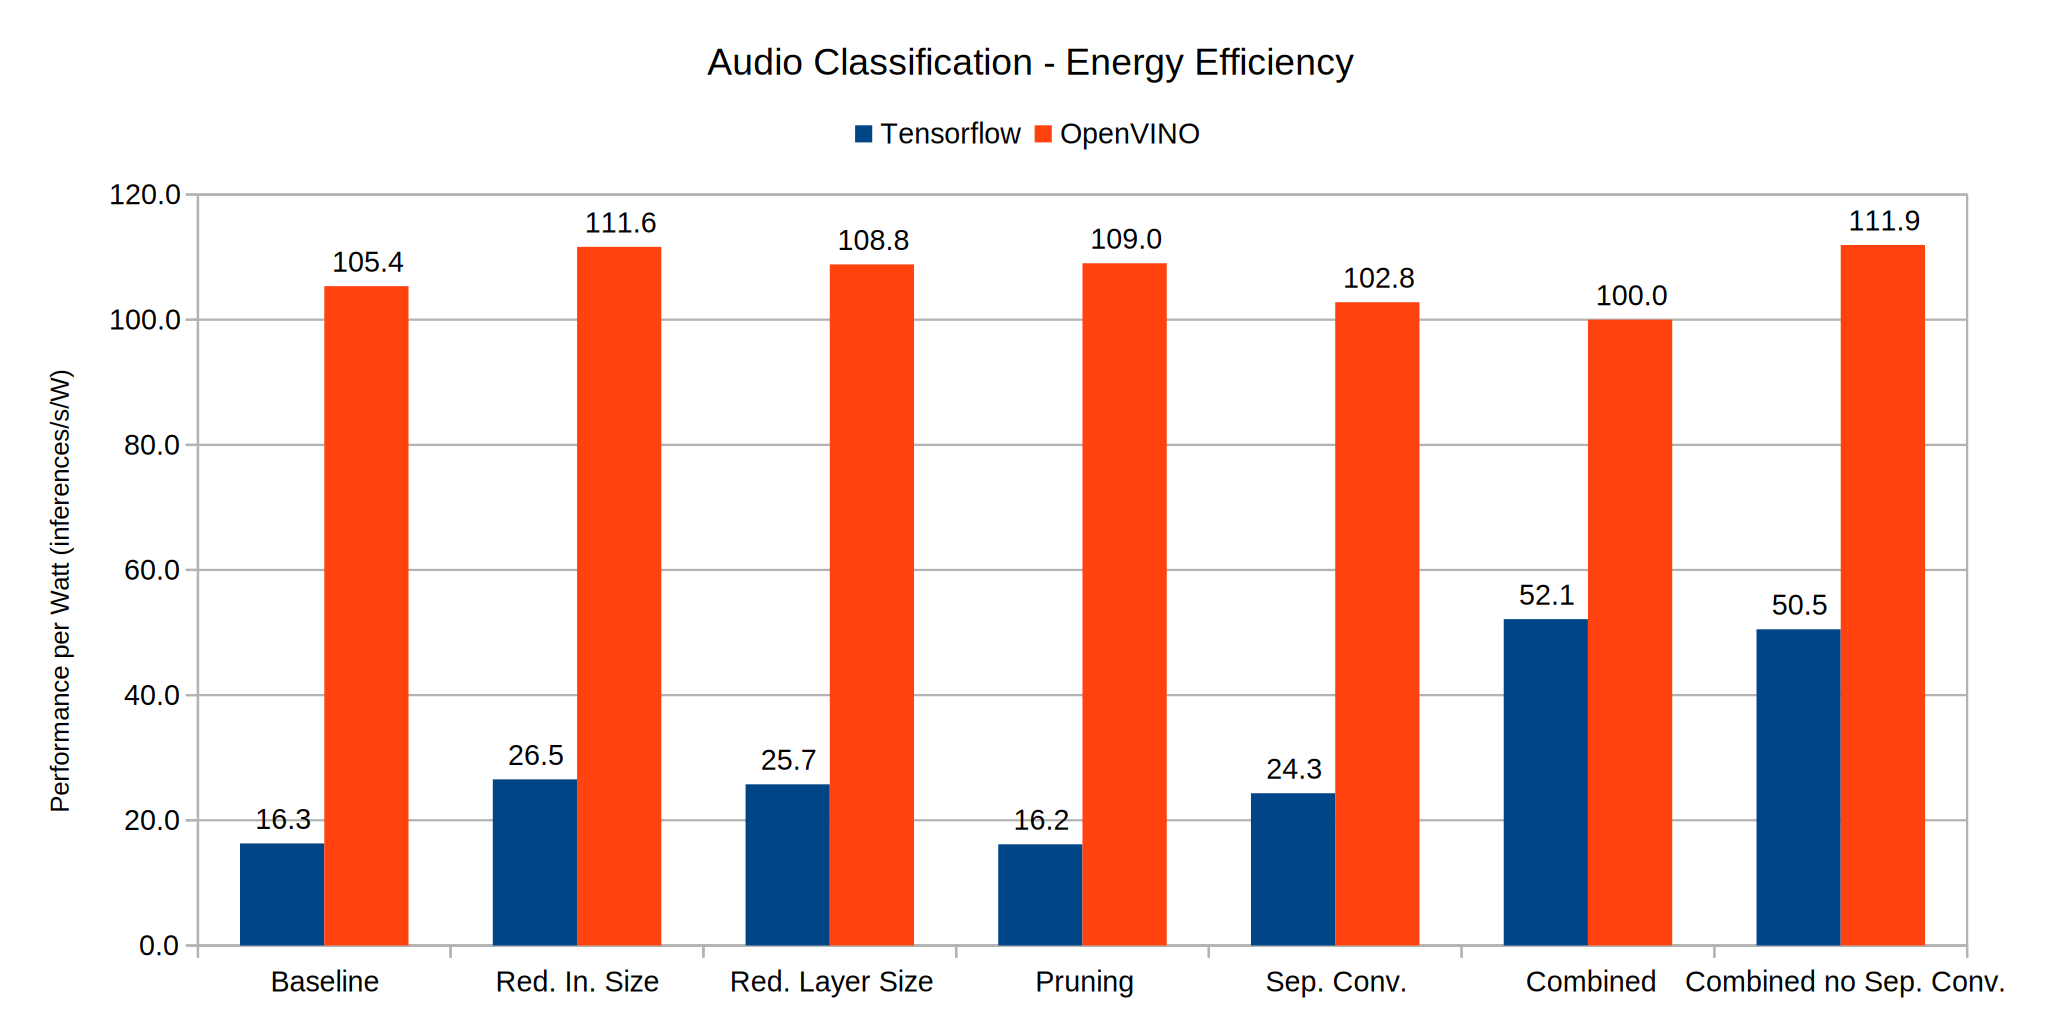
\includegraphics[scale=0.65]{ee-audio}
	\caption{Audio classification: energy efficiency comparison.}
	\label{fig:ee-audio}
\end{figure}

For the audio classification application Table \ref{tab:eet-audio} shows the power consumption metrics for each of the optimizations and Figure \ref{fig:ee-audio} shows the energy efficiency. The power consumption hovers around 6 Watts for most cases except for the separable convolution and the combined case when running with Tensorflow. When looking at the energy efficiency it follows a very similar trend as the performance chart at Figure \ref{fig:perf-audio}. Since the power consumption is so similar between all the cases this is expected. Overall OpenVINO consumes about the same power to run the application but runs much faster which makes it more energy efficient than Tensorflow, comparing the best cases for both OpenVINO has 2.15 times more performance per Watt.

\begin{table}[thbp]
\centering
\caption{Average power consumption for the fruit classification application.}
\label{tab:eet-fruit}
\begin{tabular}{|l|l|l|}
\hline
\multicolumn{1}{|c|}{\multirow{2}{*}{\textbf{Optimization}}} & \multicolumn{2}{c|}{\textbf{Power (W)}}                                           \\ \cline{2-3} 
\multicolumn{1}{|c|}{}                                       & \multicolumn{1}{c|}{\textbf{Tensorflow}} & \multicolumn{1}{c|}{\textbf{OpenVINO}} \\ \hline
Baseline                                                     & 6.1                 & 6.1               \\ \hline
Reduced Input Size                                           & 6.0                 & 6.3               \\ \hline
Reduced Layers Size                                          & 6.2                 & 6.3               \\ \hline
Pruning                                                      & 6.2                 & 6.4               \\ \hline
Separable Convolution                                        & 5.2                 & 6.0               \\ \hline
Combined                                                     & 5.2                 & 6.0               \\ \hline
Combined without Separable Convolution                       & 6.0                 & 5.9               \\ \hline
\end{tabular}
\end{table}

\begin{figure}[thbp]
	\centering
	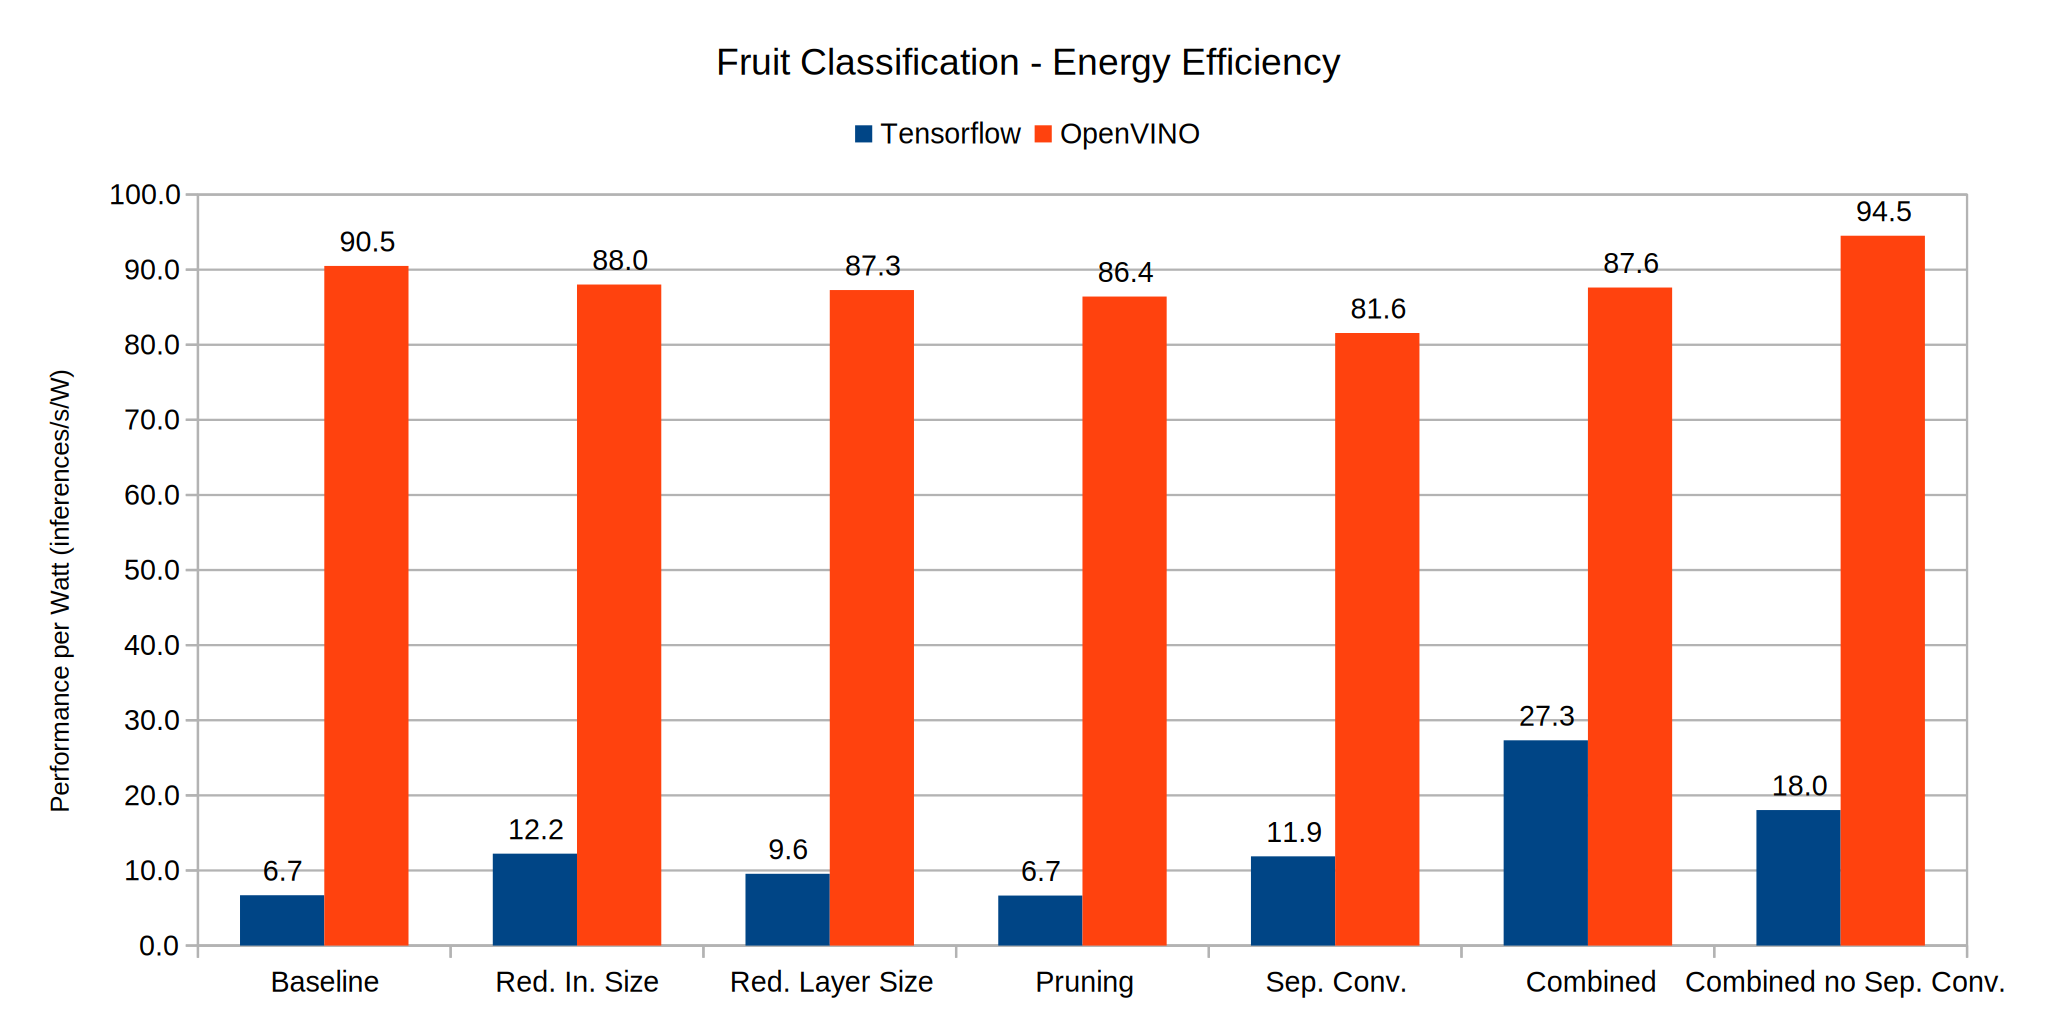
\includegraphics[scale=0.65]{ee-fruit}
	\caption{Fruit classification: energy efficiency comparison.}
	\label{fig:ee-fruit}
\end{figure}

The fruit classification application behaves very similar to the audio classification application. Table \ref{tab:eet-fruit} shows that the power consumption hovers between 6 and 6.4 Watts except when the separable convolution is used in Tensorflow. The performance per Watt follows the same trend as the audio application, Figure \ref{fig:ee-fruit} shows that when comparing the best case for each toolkit, OpenVINO is 3.46 times more energy efficient.

\begin{table}[thbp]
\centering
\caption{Average power consumption for the scene classification application.}
\label{tab:eet-scene}
\begin{tabular}{|l|l|l|}
\hline
\multicolumn{1}{|c|}{\multirow{2}{*}{\textbf{Optimization}}} & \multicolumn{2}{c|}{\textbf{Power (W)}}                                           \\ \cline{2-3} 
\multicolumn{1}{|c|}{}                                       & \multicolumn{1}{c|}{\textbf{Tensorflow}} & \multicolumn{1}{c|}{\textbf{OpenVINO}} \\ \hline
Baseline                                                     & 6.4                 & 6.2               \\ \hline
Reduced Input Size                                           & 6.4                 & 6.6               \\ \hline
Reduced Layers Size                                          & 6.2                 & 6.2               \\ \hline
Pruning                                                      & 6.2                 & 6.3               \\ \hline
Separable Convolution                                        & 5.4                 & 5.8               \\ \hline
Combined                                                     & 5.5                 & 5.7               \\ \hline
Combined without Separable Convolution                       & 6.4                 & 6.4               \\ \hline
\end{tabular}
\end{table}

\begin{figure}[thbp]
	\centering
	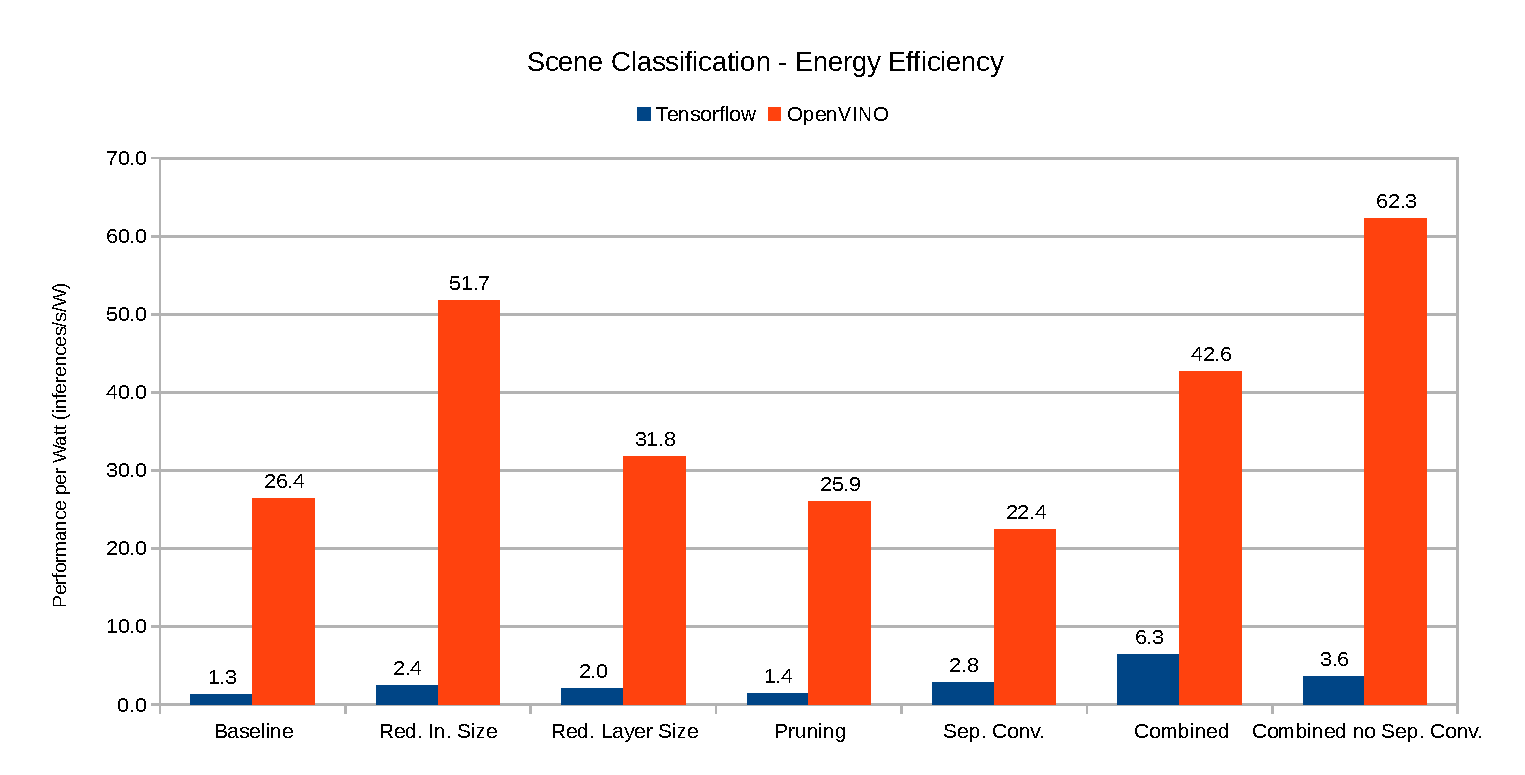
\includegraphics[scale=0.65]{ee-scene}
	\caption{Scene classification: energy efficiency comparison.}
	\label{fig:ee-scene}
\end{figure}

Finally, the scene classification application power consumption results are shown in Table \ref{tab:eet-scene}. This application consumes a little bit more power than the others, it hovers around 6.4 Watts. Similarly to the other applications, when the separable convolution optimization is present the power consumption is lower. This time OpenVINO also shows a reduction in power consumption when the separable convolution is present, something that was not seen in the other applications. Since the performance differences were more drastic the performance per Watt also shows significant differences between the different optimizations. When comparing the best case scenario for each toolkit, OpenVINO comes ahead. It is 9.89 times more energy efficient than Tensorflow.

In general, both Tensorflow and OpenVINO consume about the same amount of power. Since OpenVINO runs much faster this translates into an advantage in energy efficiency measured as performance per Watt.

\section{A Note On Quantization}

% Accuracy.

% \begin{figure}[thbp]
% 	\centering
% 	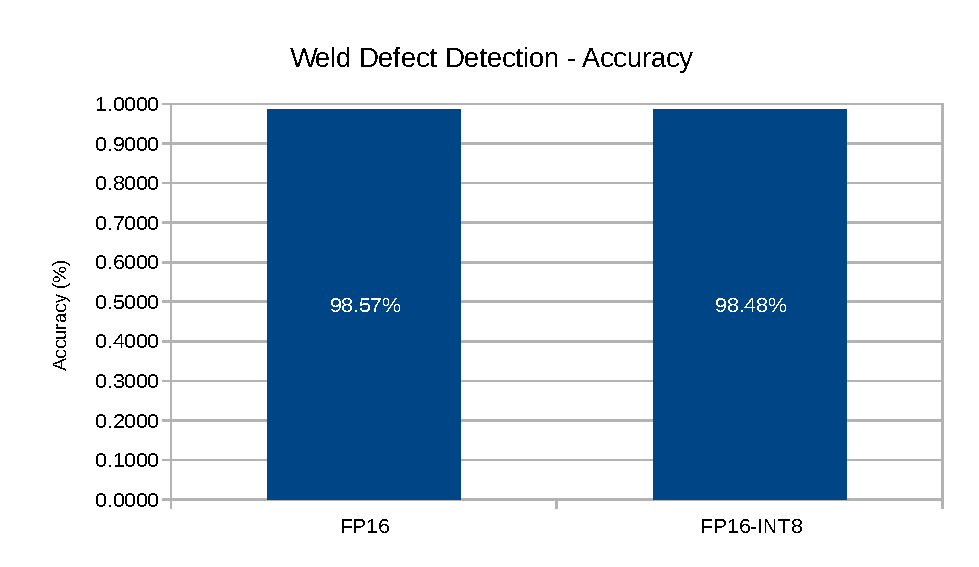
\includegraphics[scale=0.75]{acc-weld}
% 	\caption{Weld defects detection: accuracy comparison.}
% 	\label{fig:acc-weld}
% \end{figure}

% Performance.

% \begin{figure}[thbp]
% 	\centering
% 	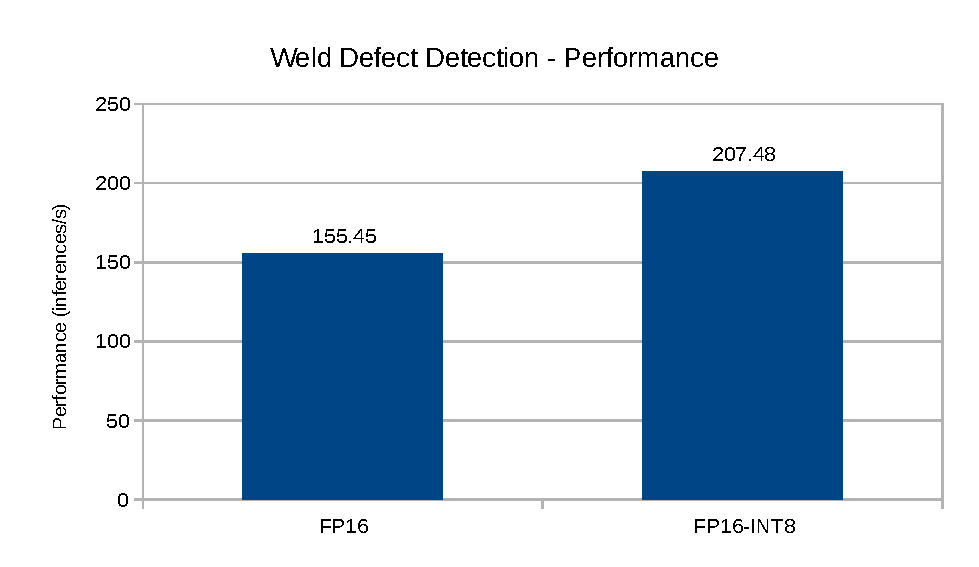
\includegraphics[scale=0.75]{perf-weld}
% 	\caption{Weld defects detection: performance comparison.}
% 	\label{fig:perf-weld}
% \end{figure}

Applying quantization as an optimization technique for neural networks can help performance. This process converts the floating point weights and biases in the layers of the neural network to integer values. In many cases doing integer calculations in hardware can be faster than doing floating point calculations, specially if the hardware supports some kind of SIMD instruction \cite{quant1}. OpenVINO has the capability execution neural networks with INT8 numbers if the hardware supports it \cite{int8}. Unfortunately the NCS2, which uses the Myriad X VPU, doesn't support INT8 operations with OpenVINO \cite{ov_sup_formats}. However most Intel processors support some kind of vector instruction set that can run multiple integer operations in parallel \cite{avx}.

The same desktop PC described in Table \ref{tab:hw_sw_details} was used to test the quantization optimization with OpenVINO. For this test the application selected is a weld porosity detection neural network \cite{weld}. It has three classes: no weld, normal weld and porosity weld. This model is available for download both as a floating point model and as an optimized version where some of the layers are quantized to INT8. The neural network was tested using a private dataset of 10 videos of approximately 20 seconds each.

\begin{figure}[thbp]
	\centering
	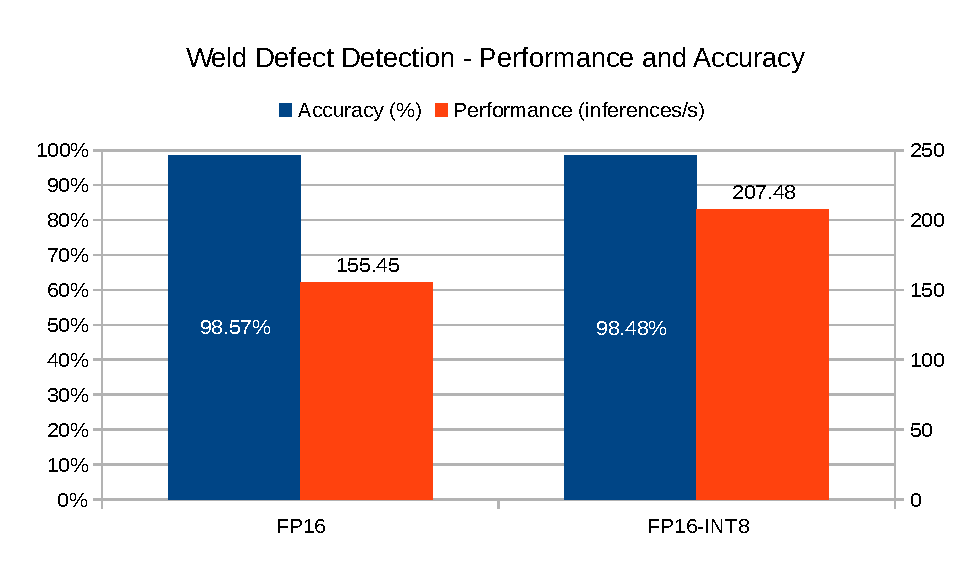
\includegraphics[scale=0.75]{comb-weld}
	\caption{Weld porosity defects detection: accuracy and performance comparison.}
	\label{fig:comb-weld}
\end{figure}

Figure \ref{fig:comb-weld} shows both the accuracy and the performance of the neural network in both cases: floating point and optimized INT8. The results show that the accuracy is barely affected by the quantization. However the performance was increased by 33.5\%.

  \chapter{Conclusions}
\label{ch:conclusion}

The Myriad X accelerator, when used in Intel's Neural Compute Stick 2 and programmed with the OpenVINO toolkit, is a loosely coupled solution that struggles to deliver high-end performance when utilizing it to do algorithmic transformations for error-tolerant applications. One of the main disadvantages of the Myriad X VPU is that is optimized for visual computing applications which mainly utilize convolutional neural networks. The tested applications, a subset of the AxBench test-suite, were not designed for this type of neural processing unit and as a result the code had to be heavily adapted to make it compatible with the OpenVINO toolkit. CNNs had to be used in an unconventional way to be able to do inference for multiple inputs in parallel in order to overcome the low performance when doing the inference for each item at a time.

To fully utilize the potential of the NCS2 it is required to have a USB3 interface, inference results are 4.6x slower when running in platforms that only support USB2. For even better performance a faster interface is needed. Intel provides PCI-E cards with Myriad X VPUs but testing those will be left for future work. The best performance gains of using the NCS2 to accelerate error-tolerant applications are seen when the device where the code is running has limited computing power capacity, and has a USB3 interface, such as the Raspberry Pi 4. Even there, only two out of five applications saw performance gains compared to the original procedural code.

There are multiple approximate computing optimization techniques that can be implemented to improve the performance and energy efficiency of neural networks such as reducing the input size, reducing the depth of CNNs, reducing the amount of neurons in a fully-connected NN, pruning the networks, using quantization to change the number representation type and number of bits and use separable convolutions in CNNs. It was demonstrated that when applying these techniques when running a neural network using the OpenVINO toolkit in the Myriad X VPU, the performance and the energy efficiency can be improved more than 2x. Also it was demonstrated that performance using an external accelerator such as the NCS2 can be improved up to 10x when compared to the same application running in the CPU of a Rapsberry Pi 4.

\section{Future Work}

In the first part of this work, algorithmic transformations were done to error-tolerant applications and mixed results were obtained. Applications were the code being substituted was simple or small saw degradation but more complex applications saw some improvement when transformed. More applications could be tested using the methods seen in this work to have a greater range of applications and have a broader perspective of what works and what does not work with this technique.

For the second part of the work, three classification applications were tested. Two saw minimal change when applying optimization techniques to improve their performance. Only one saw significant changes and this was because it was the most complex application with the biggest networks and as such, was not bottle-necked by data transfers in the NCS2. More complex applications could be tested using these techniques, this will solidify the results for the scene classification applications. For this work, only classification applications were tested, other type of applications and neural networks could be tested as well. Some examples of different networks could be recurrent neural networks and feedforward neural networks. Other examples of applications can include object detection, image segmentation, text generation, speech synthesis, face detection, etc.


  %----------------------------------------------------------------------------
  % literature
  \bibliographystyle{sty/plainurl} % for english documents
  %\bibliographystyle{plain}
  \bibliography{literatura}
  %----------------------------------------------------------------------------

  %----------------------------------------------------------------------------
  \appendix
  %----------------------------------------------------------------------------

  \chapter{Measurements for AxBench Applications}
\label{ch:appendixA}

\begin{table}[thbp]
	\centering
	\caption{Time measurements for AxBench applications (nanoseconds).}
	\label{tab:raw_time_axbench}
	\resizebox{\textwidth}{!}{%
		\begin{tabular}{|l|l|l|l|l|l|l|}
			\hline
			\textbf{Platform}              & \textbf{Measurement} & \textbf{blackscholes} & \textbf{inversek2j} & \textbf{jmeint} & \textbf{kmeans} & \textbf{sobel} \\ \hline
			\multirow{8}{*}{\textbf{PC}}   & Original code        & 12224                 & 70804               & 36483           & 149084          & 130821         \\ \cline{2-7} 
			& OV CPU (NN 1)        & 4108                  & 9698                & 22572           & 847731          & 68636          \\ \cline{2-7} 
			& OV MYRIAD (NN 1)     & 32129                 & 86233               & 326174          & 5707387         & 450249         \\ \cline{2-7} 
			& OV MYRIAD USB2       & 147127                & 402953              & 1872465         & 33734206        & 1833880        \\ \cline{2-7} 
			& OV CPU (NN 2)        & 6600                  & 11847               & 24721           & 846761          & 76582          \\ \cline{2-7} 
			& OV MYRIAD (NN 2)     & 34616                 & 82474               & 340231          & 5667970         & 578209         \\ \cline{2-7} 
			& OV CPU (NN 3)        & 7969                  & 12830               & 26571           & 848350          & 81531          \\ \cline{2-7} 
			& OV MYRIAD (NN 3)     & 40629                 & 90092               & 361311          & 5696227         & 745561         \\ \hline
			\multirow{2}{*}{\textbf{RPi3}} & Original code        & 152695                & 607658              & 190794          & 2053881         & 905649         \\ \cline{2-7} 
			& OV MYRIAD            & 172422                & 471115              & 2257072         & 44081815        & 2313934        \\ \hline
			\multirow{3}{*}{\textbf{RPi4}} & Original code        & 58007                 & 293278              & 113053          & 565203          & 555553         \\ \cline{2-7} 
			& OV MYRIAD            & 45608                 & 120741              & 469744          & 12460832        & 661277         \\ \cline{2-7} 
			& OV MYRIAD USB2       & 184947                & 496012              & 2506141         & 48206986        & 2424196        \\ \hline
		\end{tabular}%
	}
\end{table}

\begin{table}[thbp]
	\centering
	\caption{Error measurements for AxBench applications.}
	\label{tab:error_axbench}
	\resizebox{\textwidth}{!}{%
		\begin{tabular}{|l|l|l|l|l|l|l|l|}
			\hline
			\textbf{Application}                   & \textbf{Error type} & \textbf{CPU (NN 1)} & \textbf{MYRIAD (NN 1)} & \textbf{CPU (NN 2)} & \textbf{MYRIAD (NN 2)} & \textbf{CPU (NN 3)} & \textbf{MYRIAD (NN 3)} \\ \hline
			\multirow{3}{*}{\textbf{blackscholes}} & WMAPE               & 3.03                & 5.54                   & 0.85                & 2.93                   & 0.83                & 3.93                   \\ \cline{2-8} 
			& MAPE                & 18.73               & 23.83                  & 12.21               & 15.58                  & 9.80                & 16.59                  \\ \cline{2-8} 
			& MSE                 & 5.37E-04            & 1.47E-03               & 4.53E-05            & 4.09E-04               & 3.35E-05            & 6.57E-04               \\ \hline
			\multirow{3}{*}{\textbf{inversek2j}}   & WMAPE               & 4.34                & 4.32                   & 1.92                & 1.99                   & 1.45                & 1.55                   \\ \cline{2-8} 
			& MAPE                & 10.84               & 10.81                  & 6.14                & 6.27                   & 5.18                & 5.35                   \\ \cline{2-8} 
			& MSE                 & 1.90E-01            & 1.90E-01               & 4.38E-02            & 4.69E-02               & 2.76E-02            & 3.15E-02               \\ \hline
			\multirow{3}{*}{\textbf{kmeans}}       & WMAPE               & 4.07                & 4.07                   & 3.99                & 3.97                   & 1.18                & 1.27                   \\ \cline{2-8} 
			& MAPE                & 5.23                & 5.24                   & 5.21                & 5.23                   & 1.31                & 1.40                   \\ \cline{2-8} 
			& MSE                 & 17912               & 17778                  & 16008               & 16018                  & 4927                & 5332                   \\ \hline
			\multirow{3}{*}{\textbf{sobel}}        & WMAPE               & 8.01                & 8.31                   & 3.80                & 4.40                   & 5.74                & 5.60                   \\ \cline{2-8} 
			& MAPE                & 16.00               & 17.56                  & 9.29                & 11.53                  & 18.40               & 17.48                  \\ \cline{2-8} 
			& MSE                 & 15572               & 15915                  & 4942                & 5230                   & 6752                & 6840                   \\ \hline
			\textbf{jmeint}                        & Miss rate           & 15.65               & 15.66                  & 14.2                & 14.17                  & 14.18               & 14.23                  \\ \hline
		\end{tabular}%
	}
\end{table}


  %----------------------------------------------------------------------------
  \backmatter
  %----------------------------------------------------------------------------

  \printindex                % insert index into document. Don't forget to call
                             % "makeindex filename" first.
\end{document}
